% !TEX TS-program = xelatex
% !TEX encoding = UTF-8
% !Mode:: "TeX:UTF-8"

\documentclass[onecolumn,oneside]{BUPTHomework}

\author{胡玉斌,曾维恺,石超}
\sid{}
\title{SQL Server 容灾实验}
\coursecode{3131100787}
\coursename{网络存储与容灾技术}

\begin{document}
  \maketitle

  \section{实验环境}

  \begin{itemize}
    \item Windows 10 Pro
    \item SQL Server 2019
  \end{itemize}

  \subsection{安装 SQL Server 2019}

  在安装中心,安装SQL Server实例。
  由于我们之后需要主体服务器,镜像服务器,见证服务器,且我们只有一台主机来模拟实验,所以需要创建三个实例。
  见Figure \ref{pic1}。

  \begin{itemize}
    \item BUPTPRINCIPAL: 主体服务器
    \item BUPTMIRROR: 镜像服务器
    \item BUPTWITNESS: 见证服务器
  \end{itemize}

  \begin{figure}[h]
    \centering
    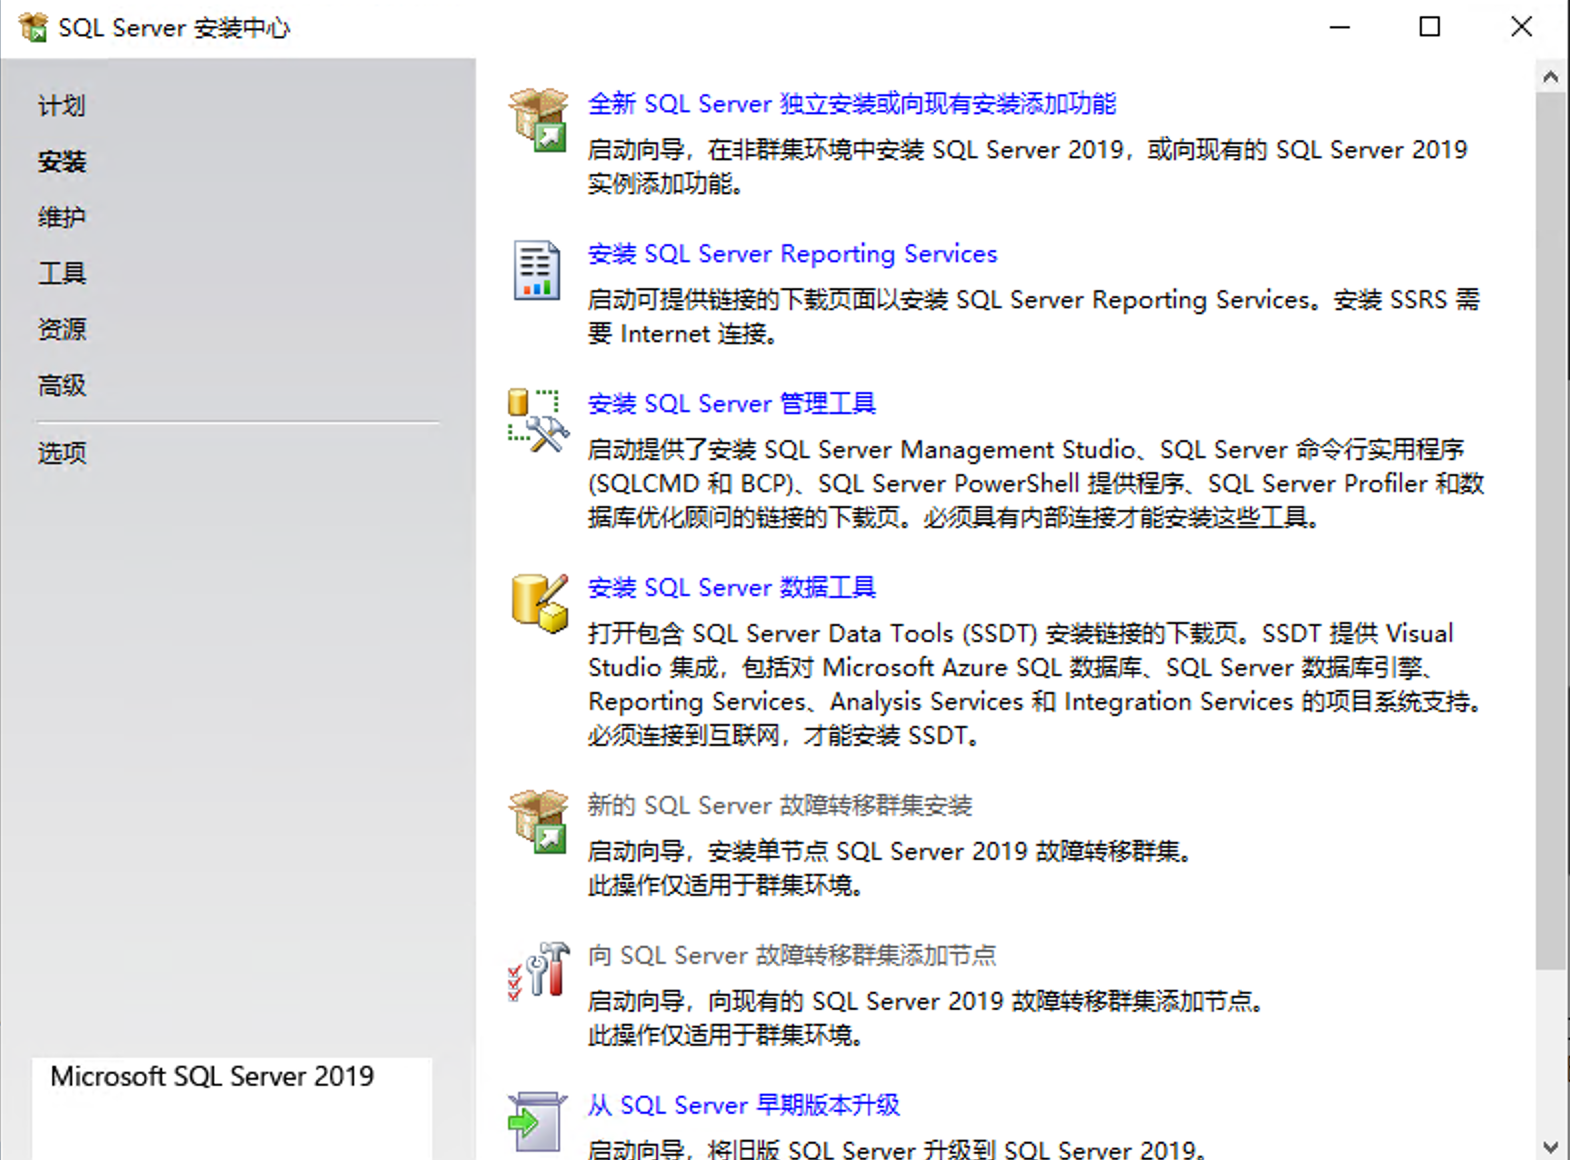
\includegraphics[width=0.70\textwidth]{image/pic1.png}
    \caption{SQL Server 安装中心}
    \label{pic1}
  \end{figure}

  \subsection{SSMS}

  SQL Server Management Studio (SSMS) 是一种集成环境,用于管理从 SQL Server 到 Azure SQL 数据库的任何 SQL 基础结构。
  SSMS 提供用于配置、监视和管理 SQL Server 和数据库实例的工具。
  使用 SSMS 部署、监视和升级应用程序使用的数据层组件,以及生成查询和脚本。

  \section{备份}

  首先我们先在主体服务器上新建一个数据库,新建一张表,存储数据,以备验证。
  见Figure \ref{pic2}。

  \begin{figure}[h]
    \centering
    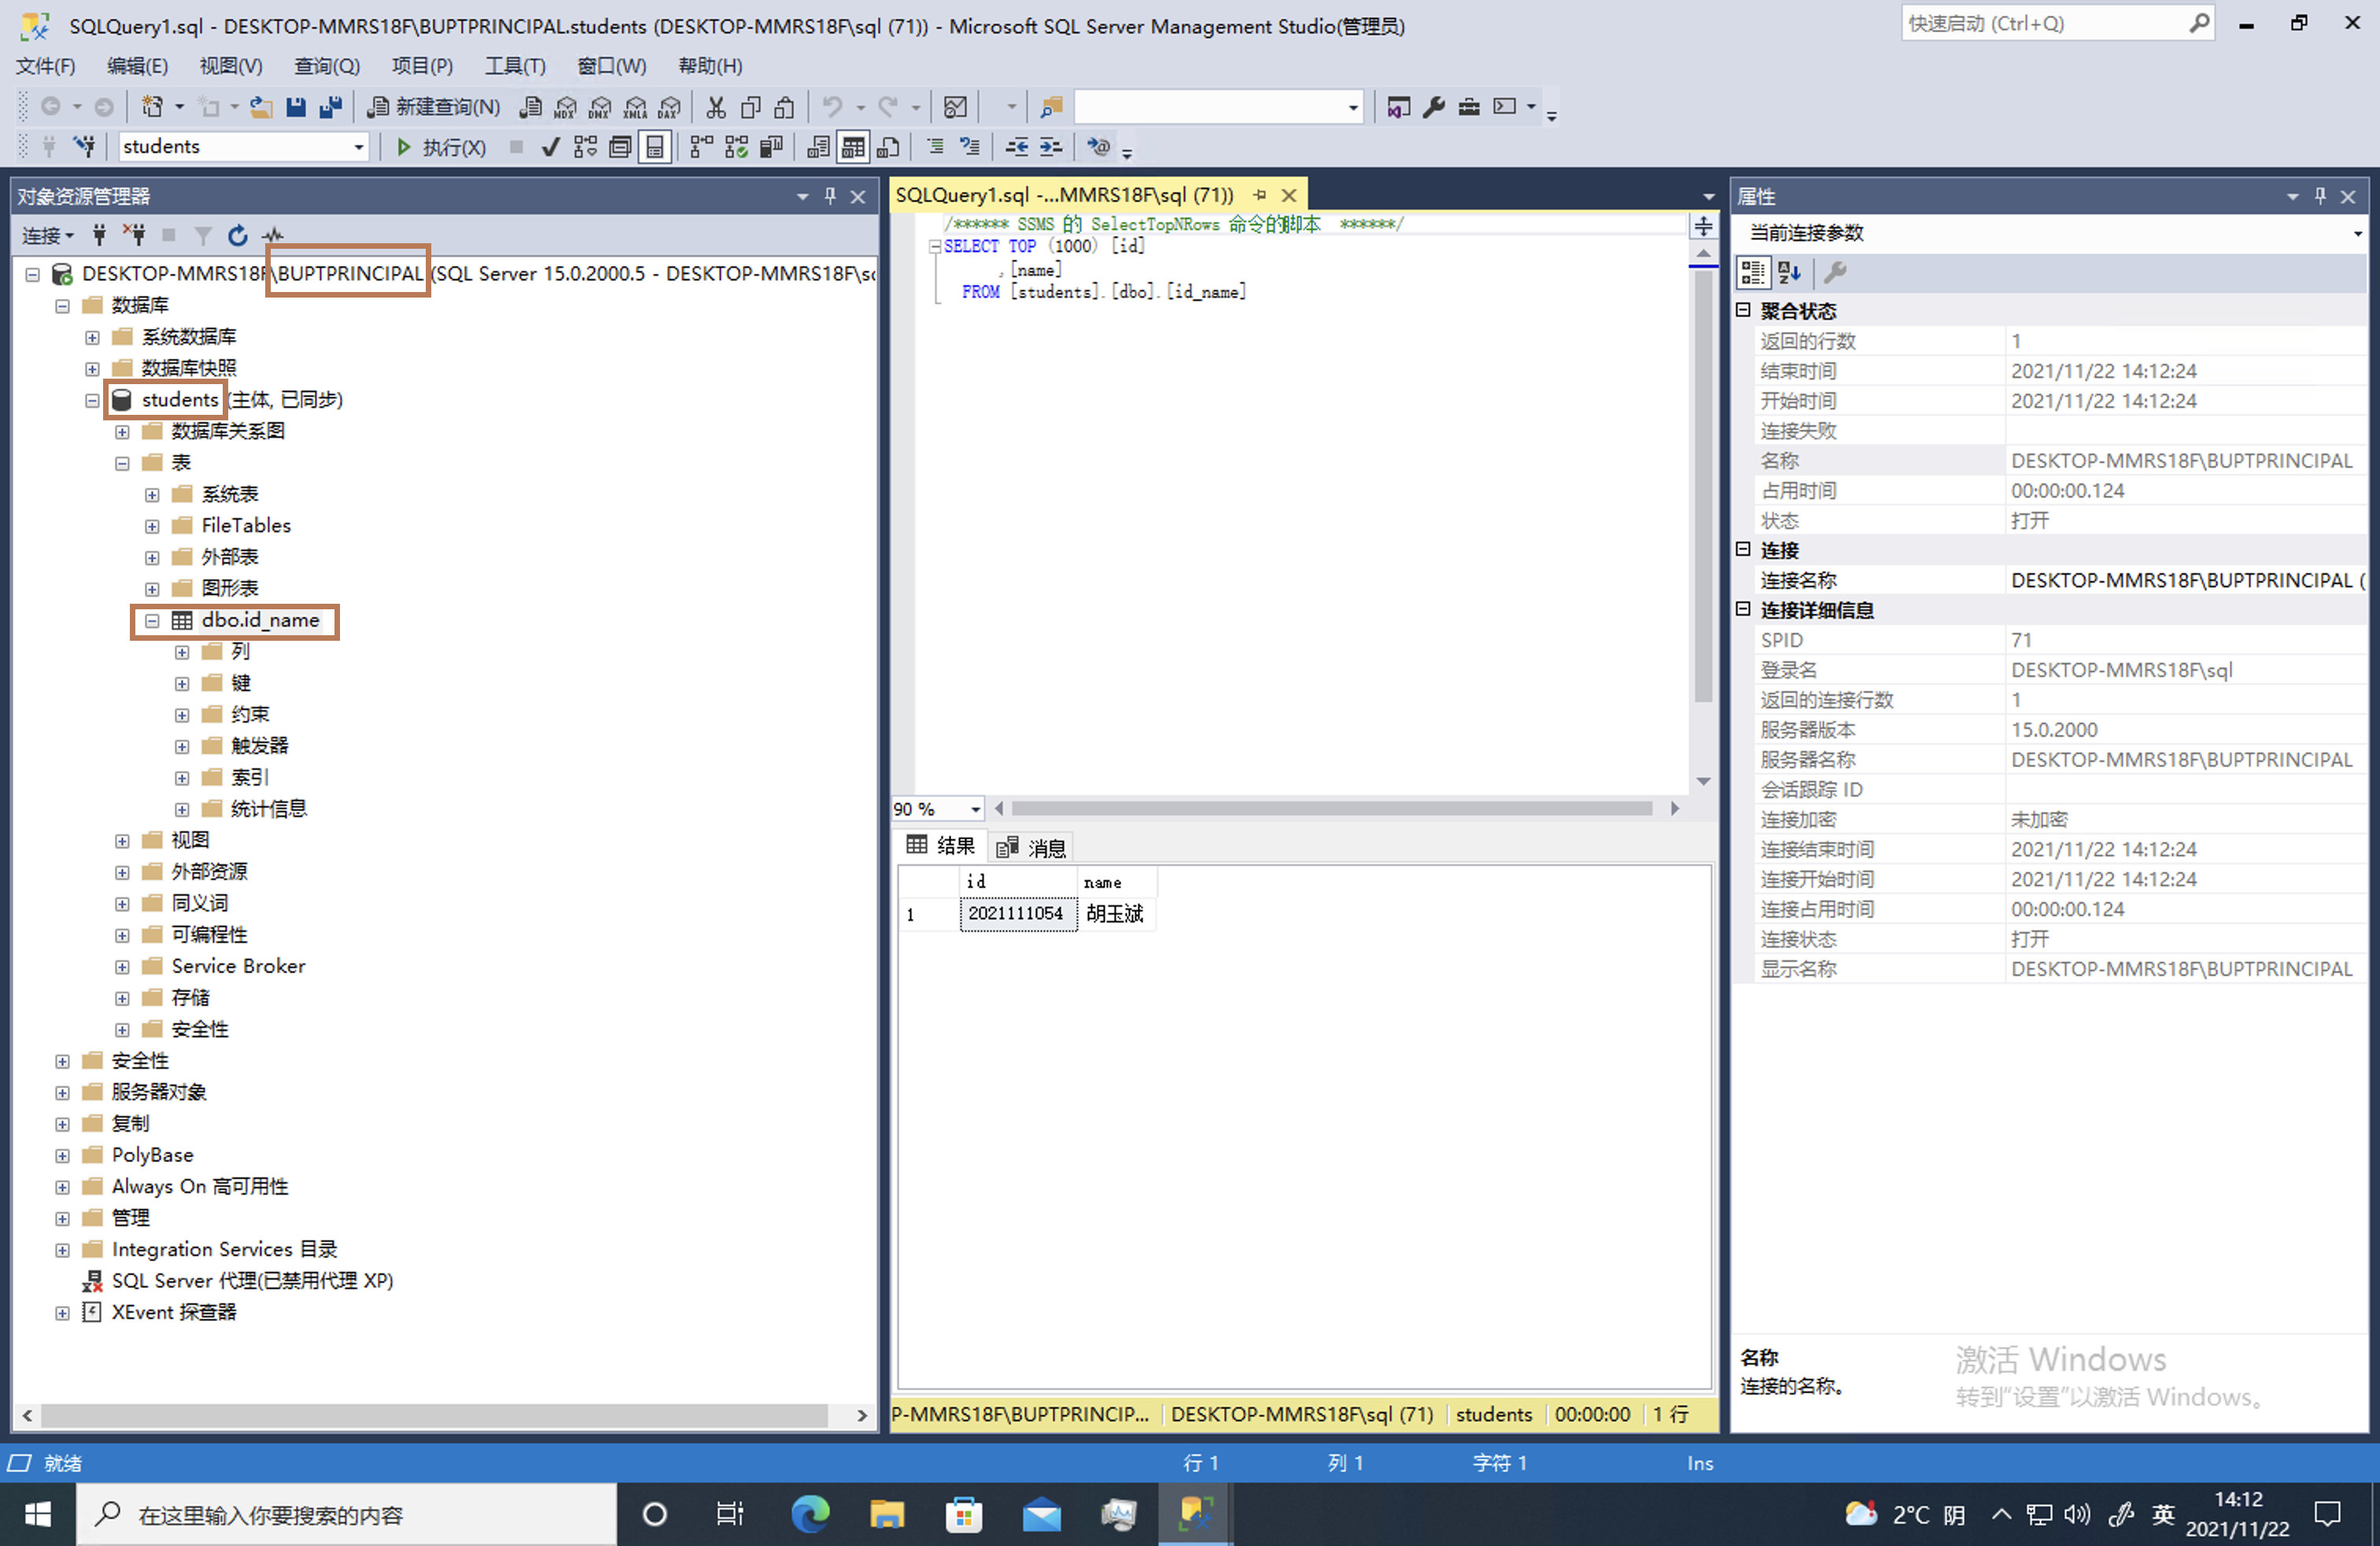
\includegraphics[width=0.70\textwidth]{image/pic2.png}
    \caption{准备数据库}
    \label{pic2}
  \end{figure}

  \subsection{数据库完整备份}

  将主体服务器(BUPTPRINCIPAL)数据库(students)进行完整备份。
  见Figure \ref{pic3}。

  \begin{figure}[h]
    \centering
    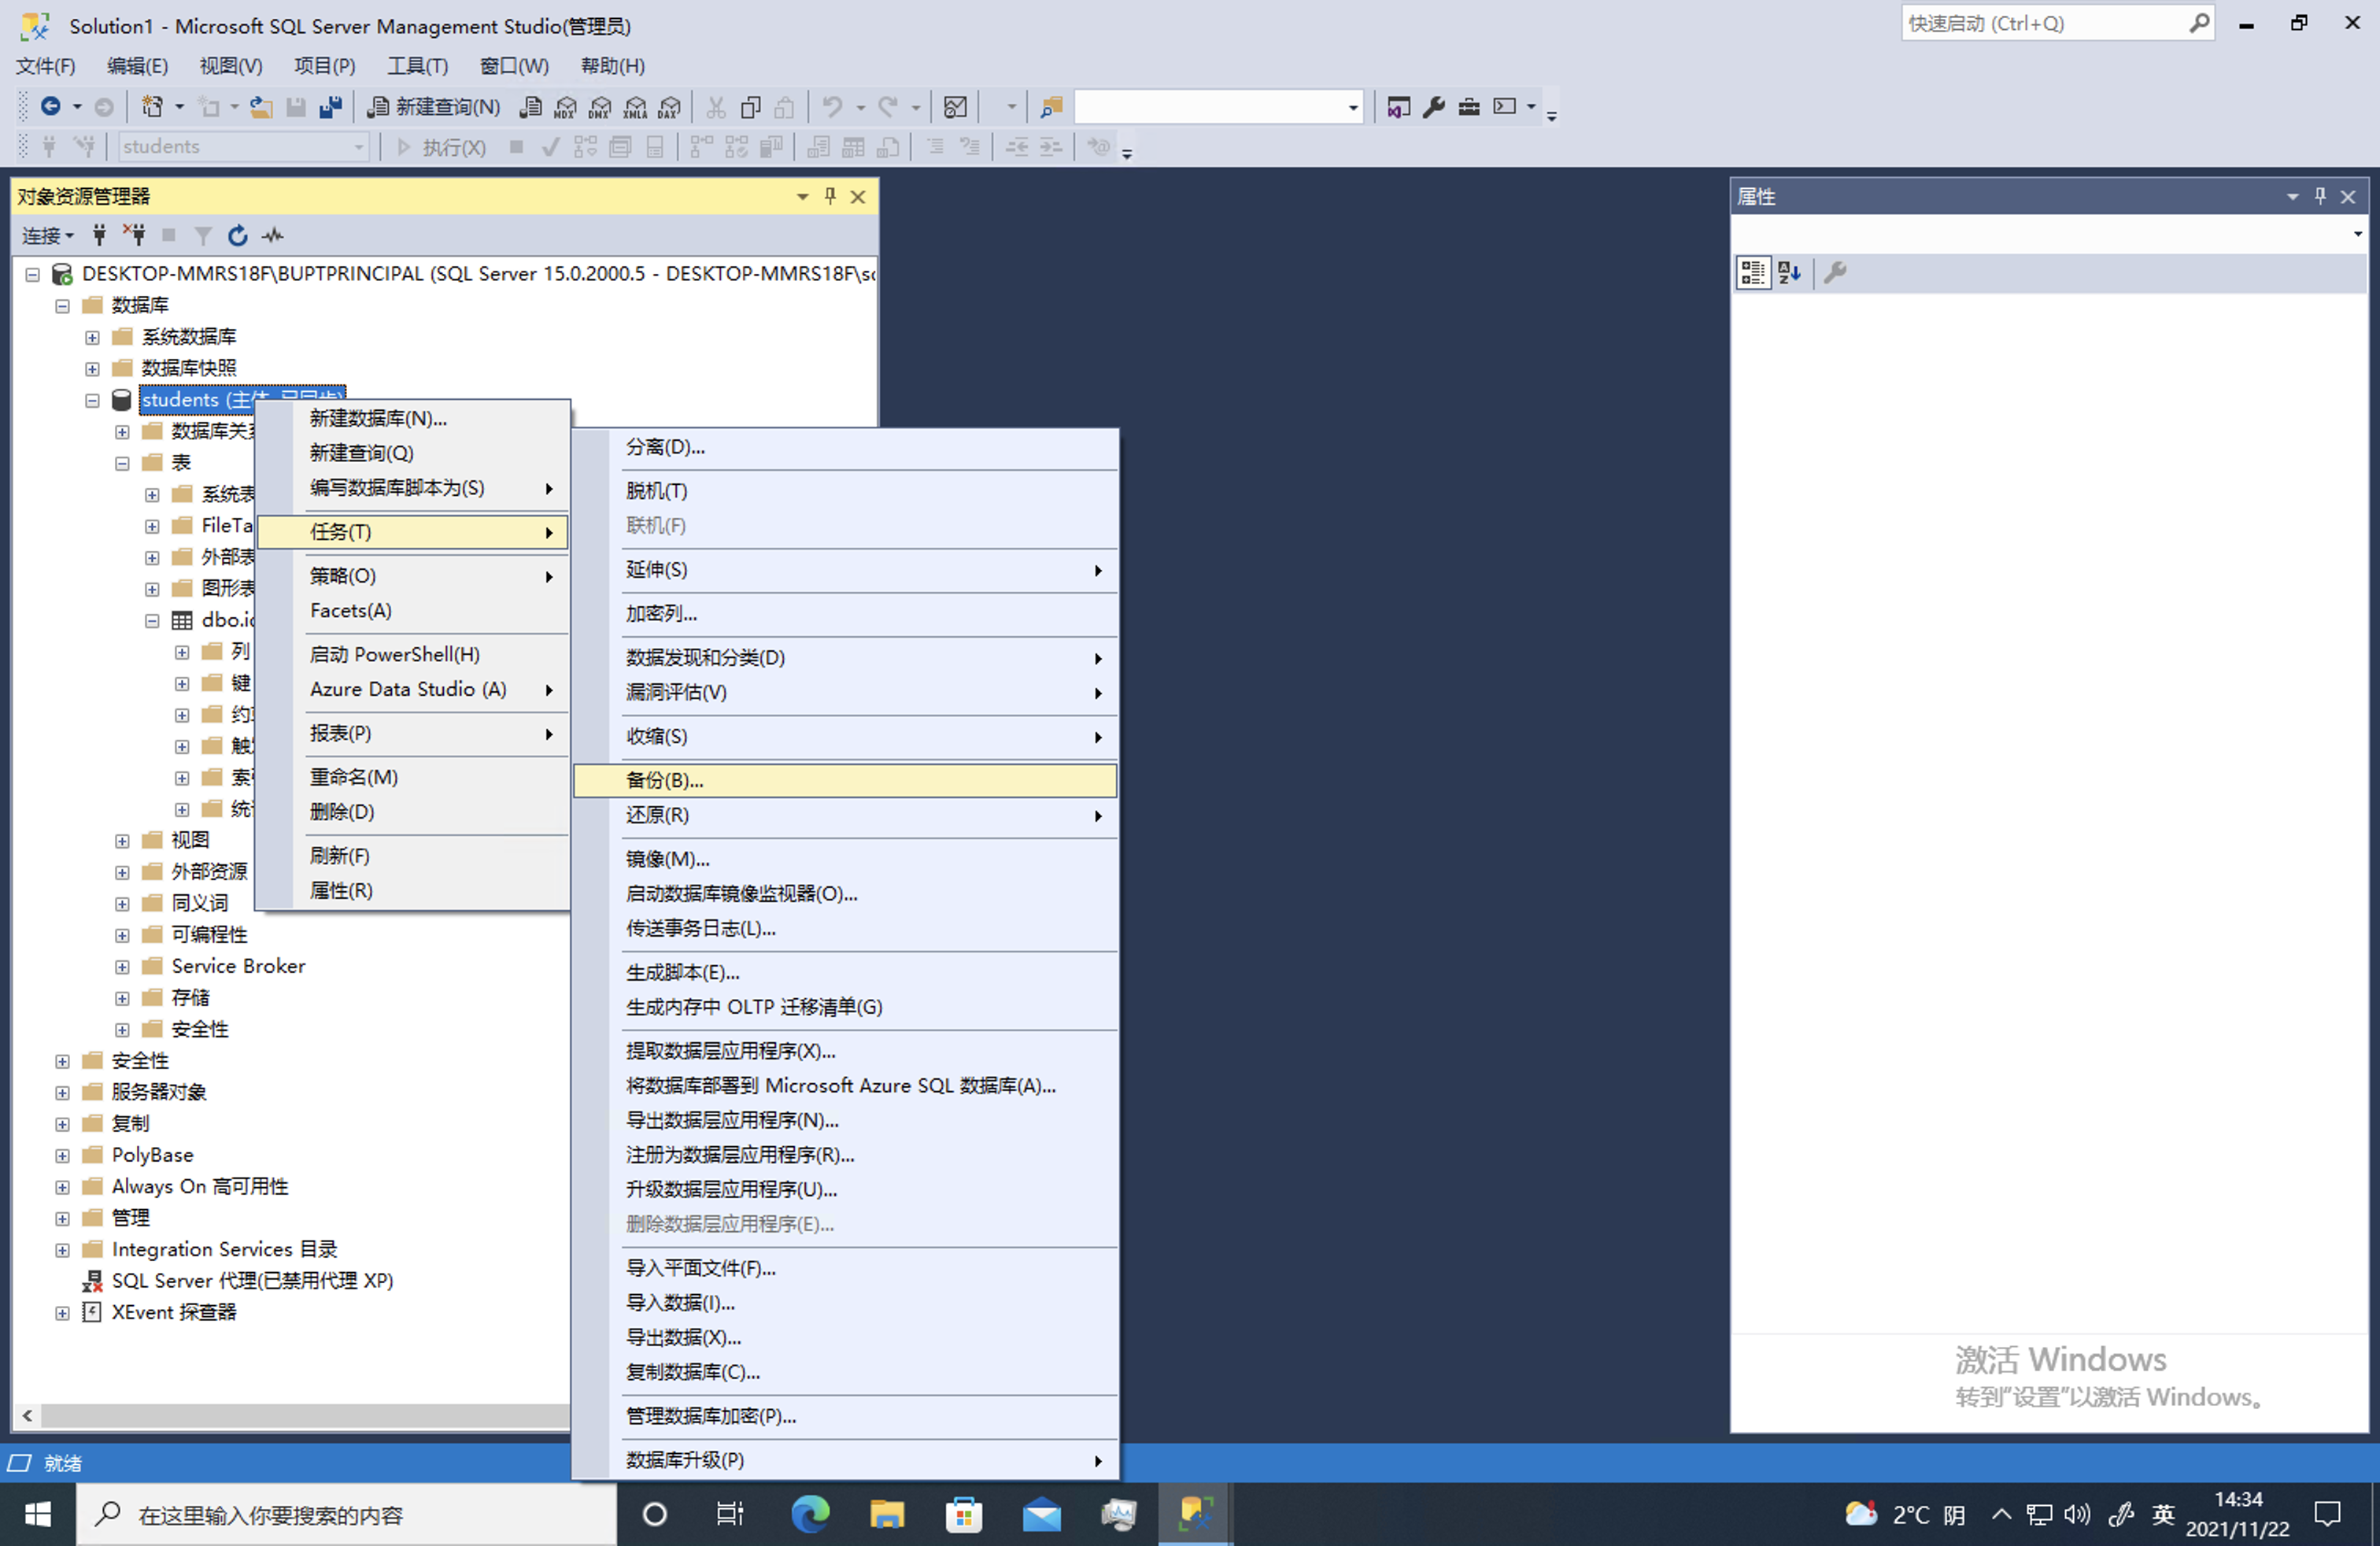
\includegraphics[width=0.70\textwidth]{image/pic3.png}
    \caption{准备数据库}
    \label{pic3}
  \end{figure}

  在 \textit{备份类型} 中选择 \textit{完整}。
  见Figure \ref{pic4}。

  \newpage

  \begin{figure}[h]
    \centering
    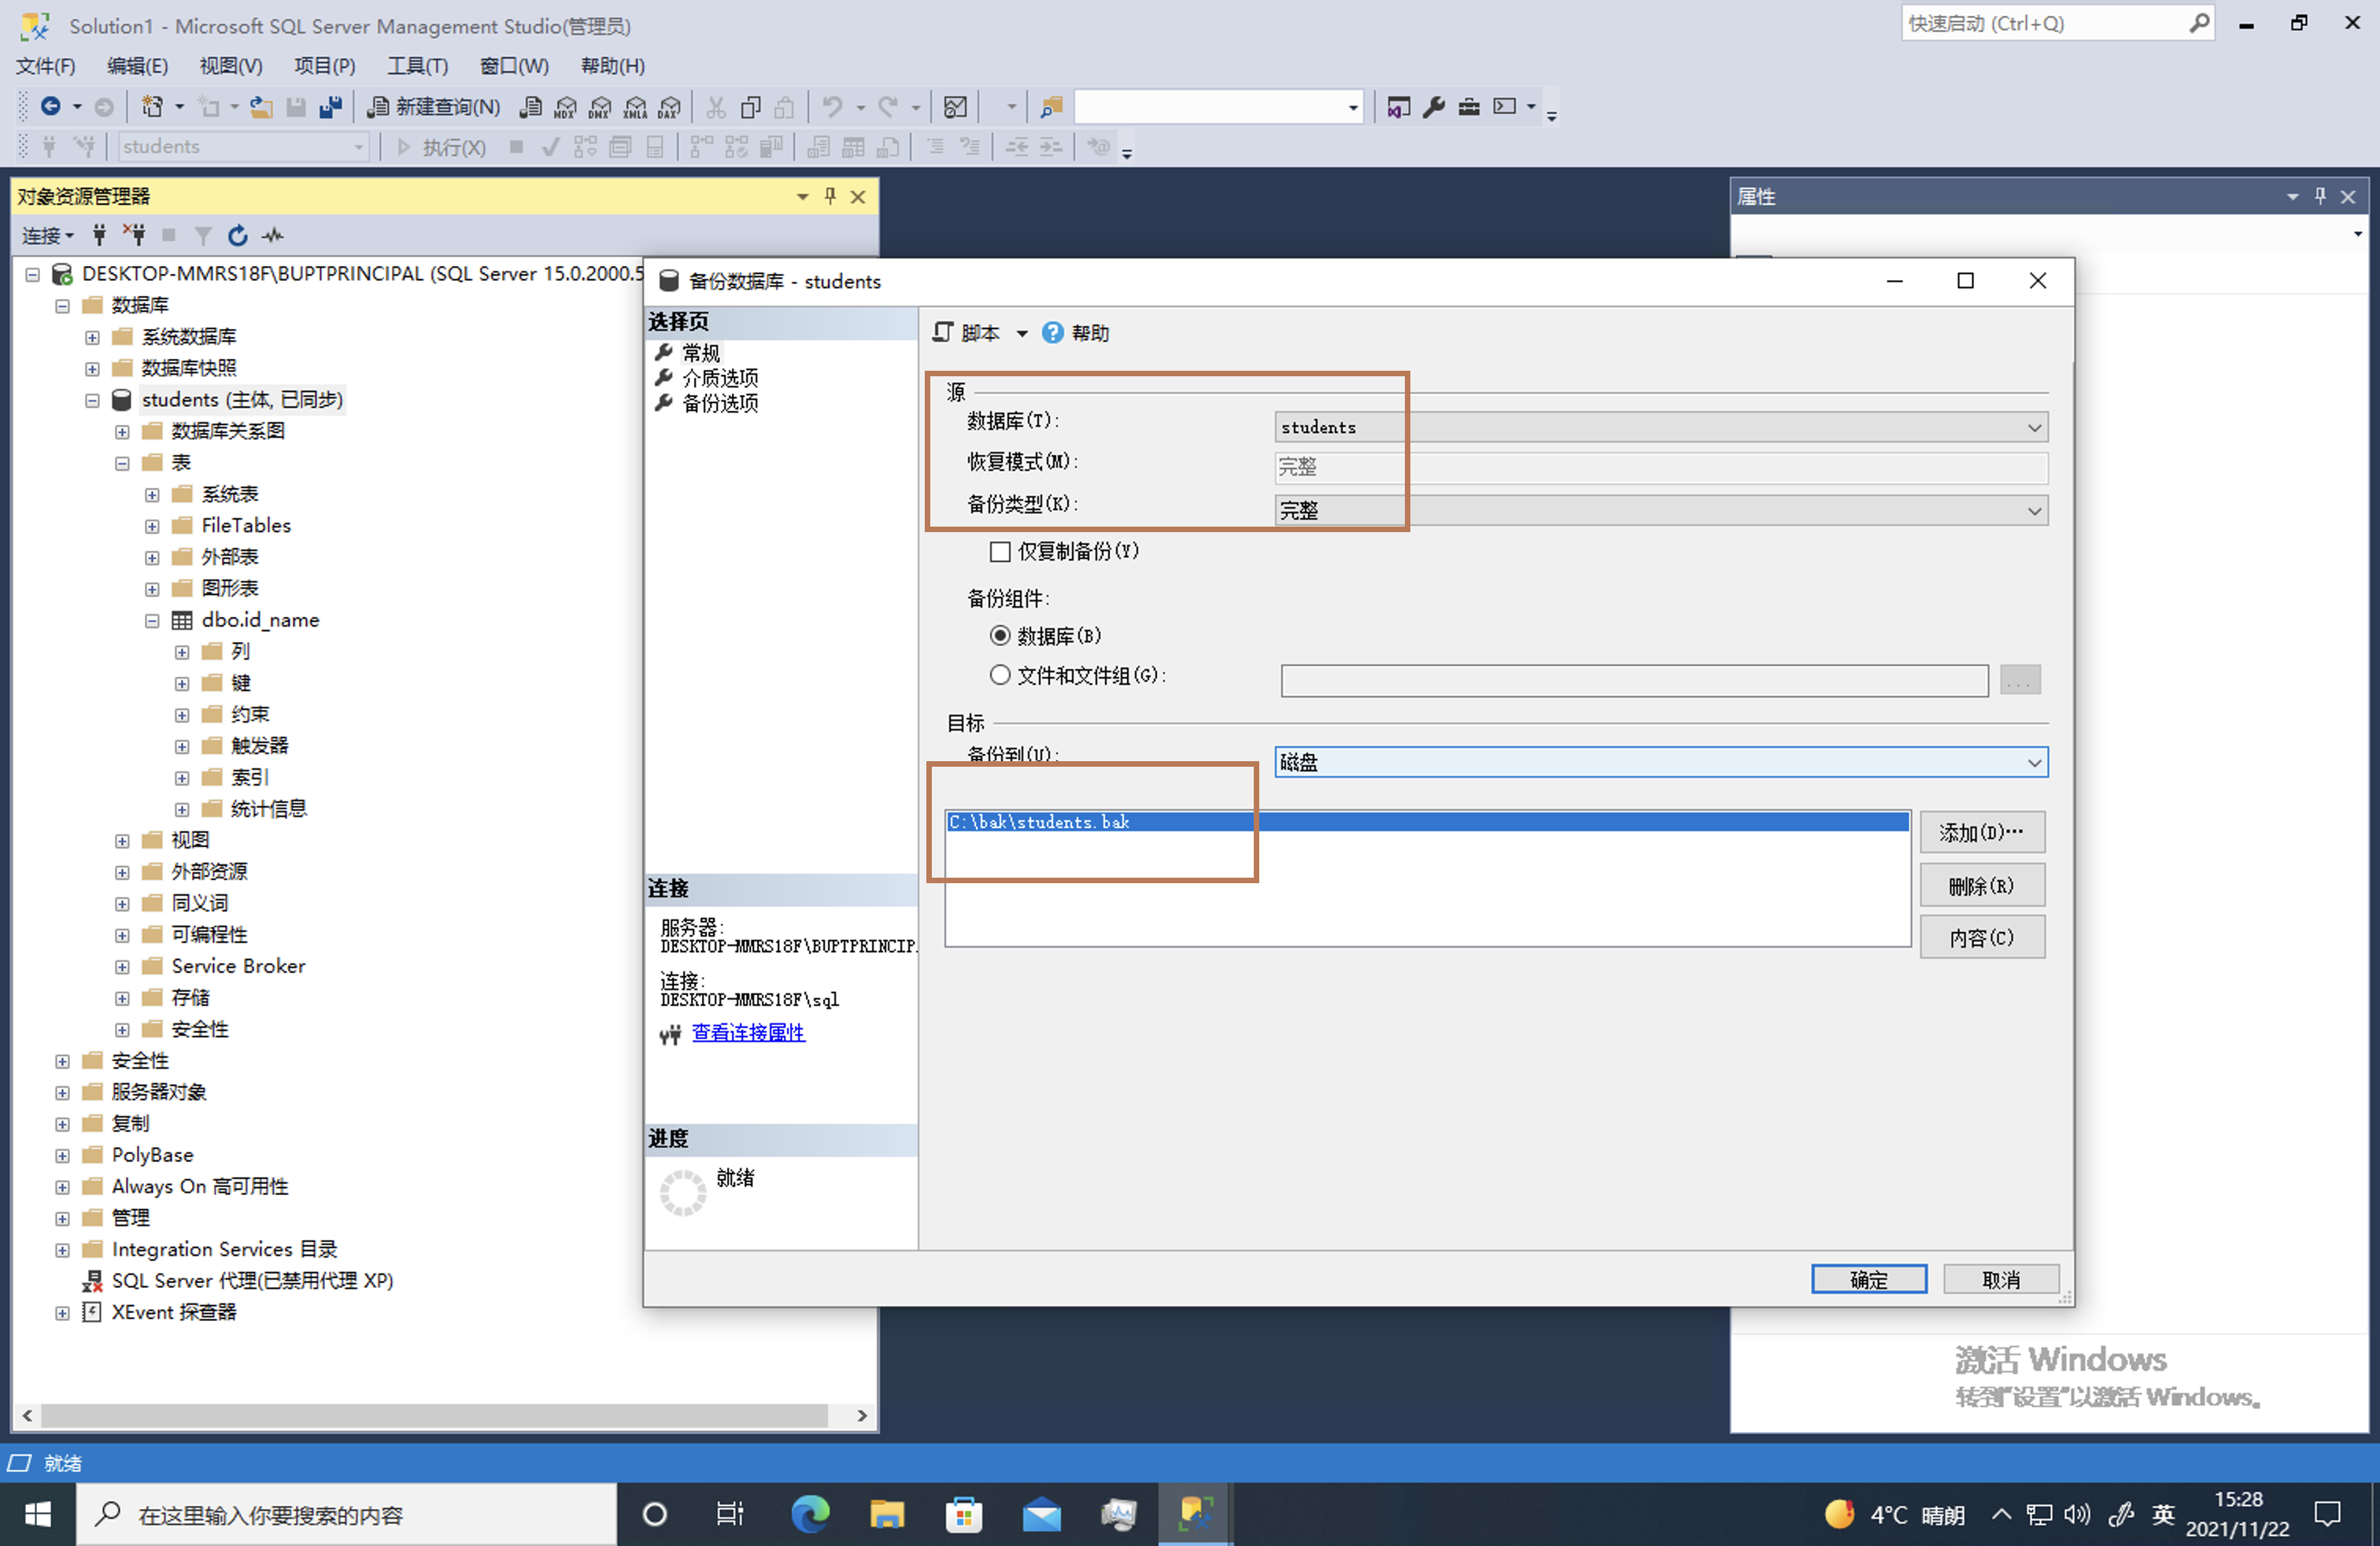
\includegraphics[width=0.70\textwidth]{image/pic4.png}
    \caption{完整备份}
    \label{pic4}
  \end{figure}

  \subsection{数据库差异备份}

  将主体服务器(BUPTPRINCIPAL)数据库(students)进行差异备份。
  见Figure \ref{pic5}。

  \begin{figure}[h]
    \centering
    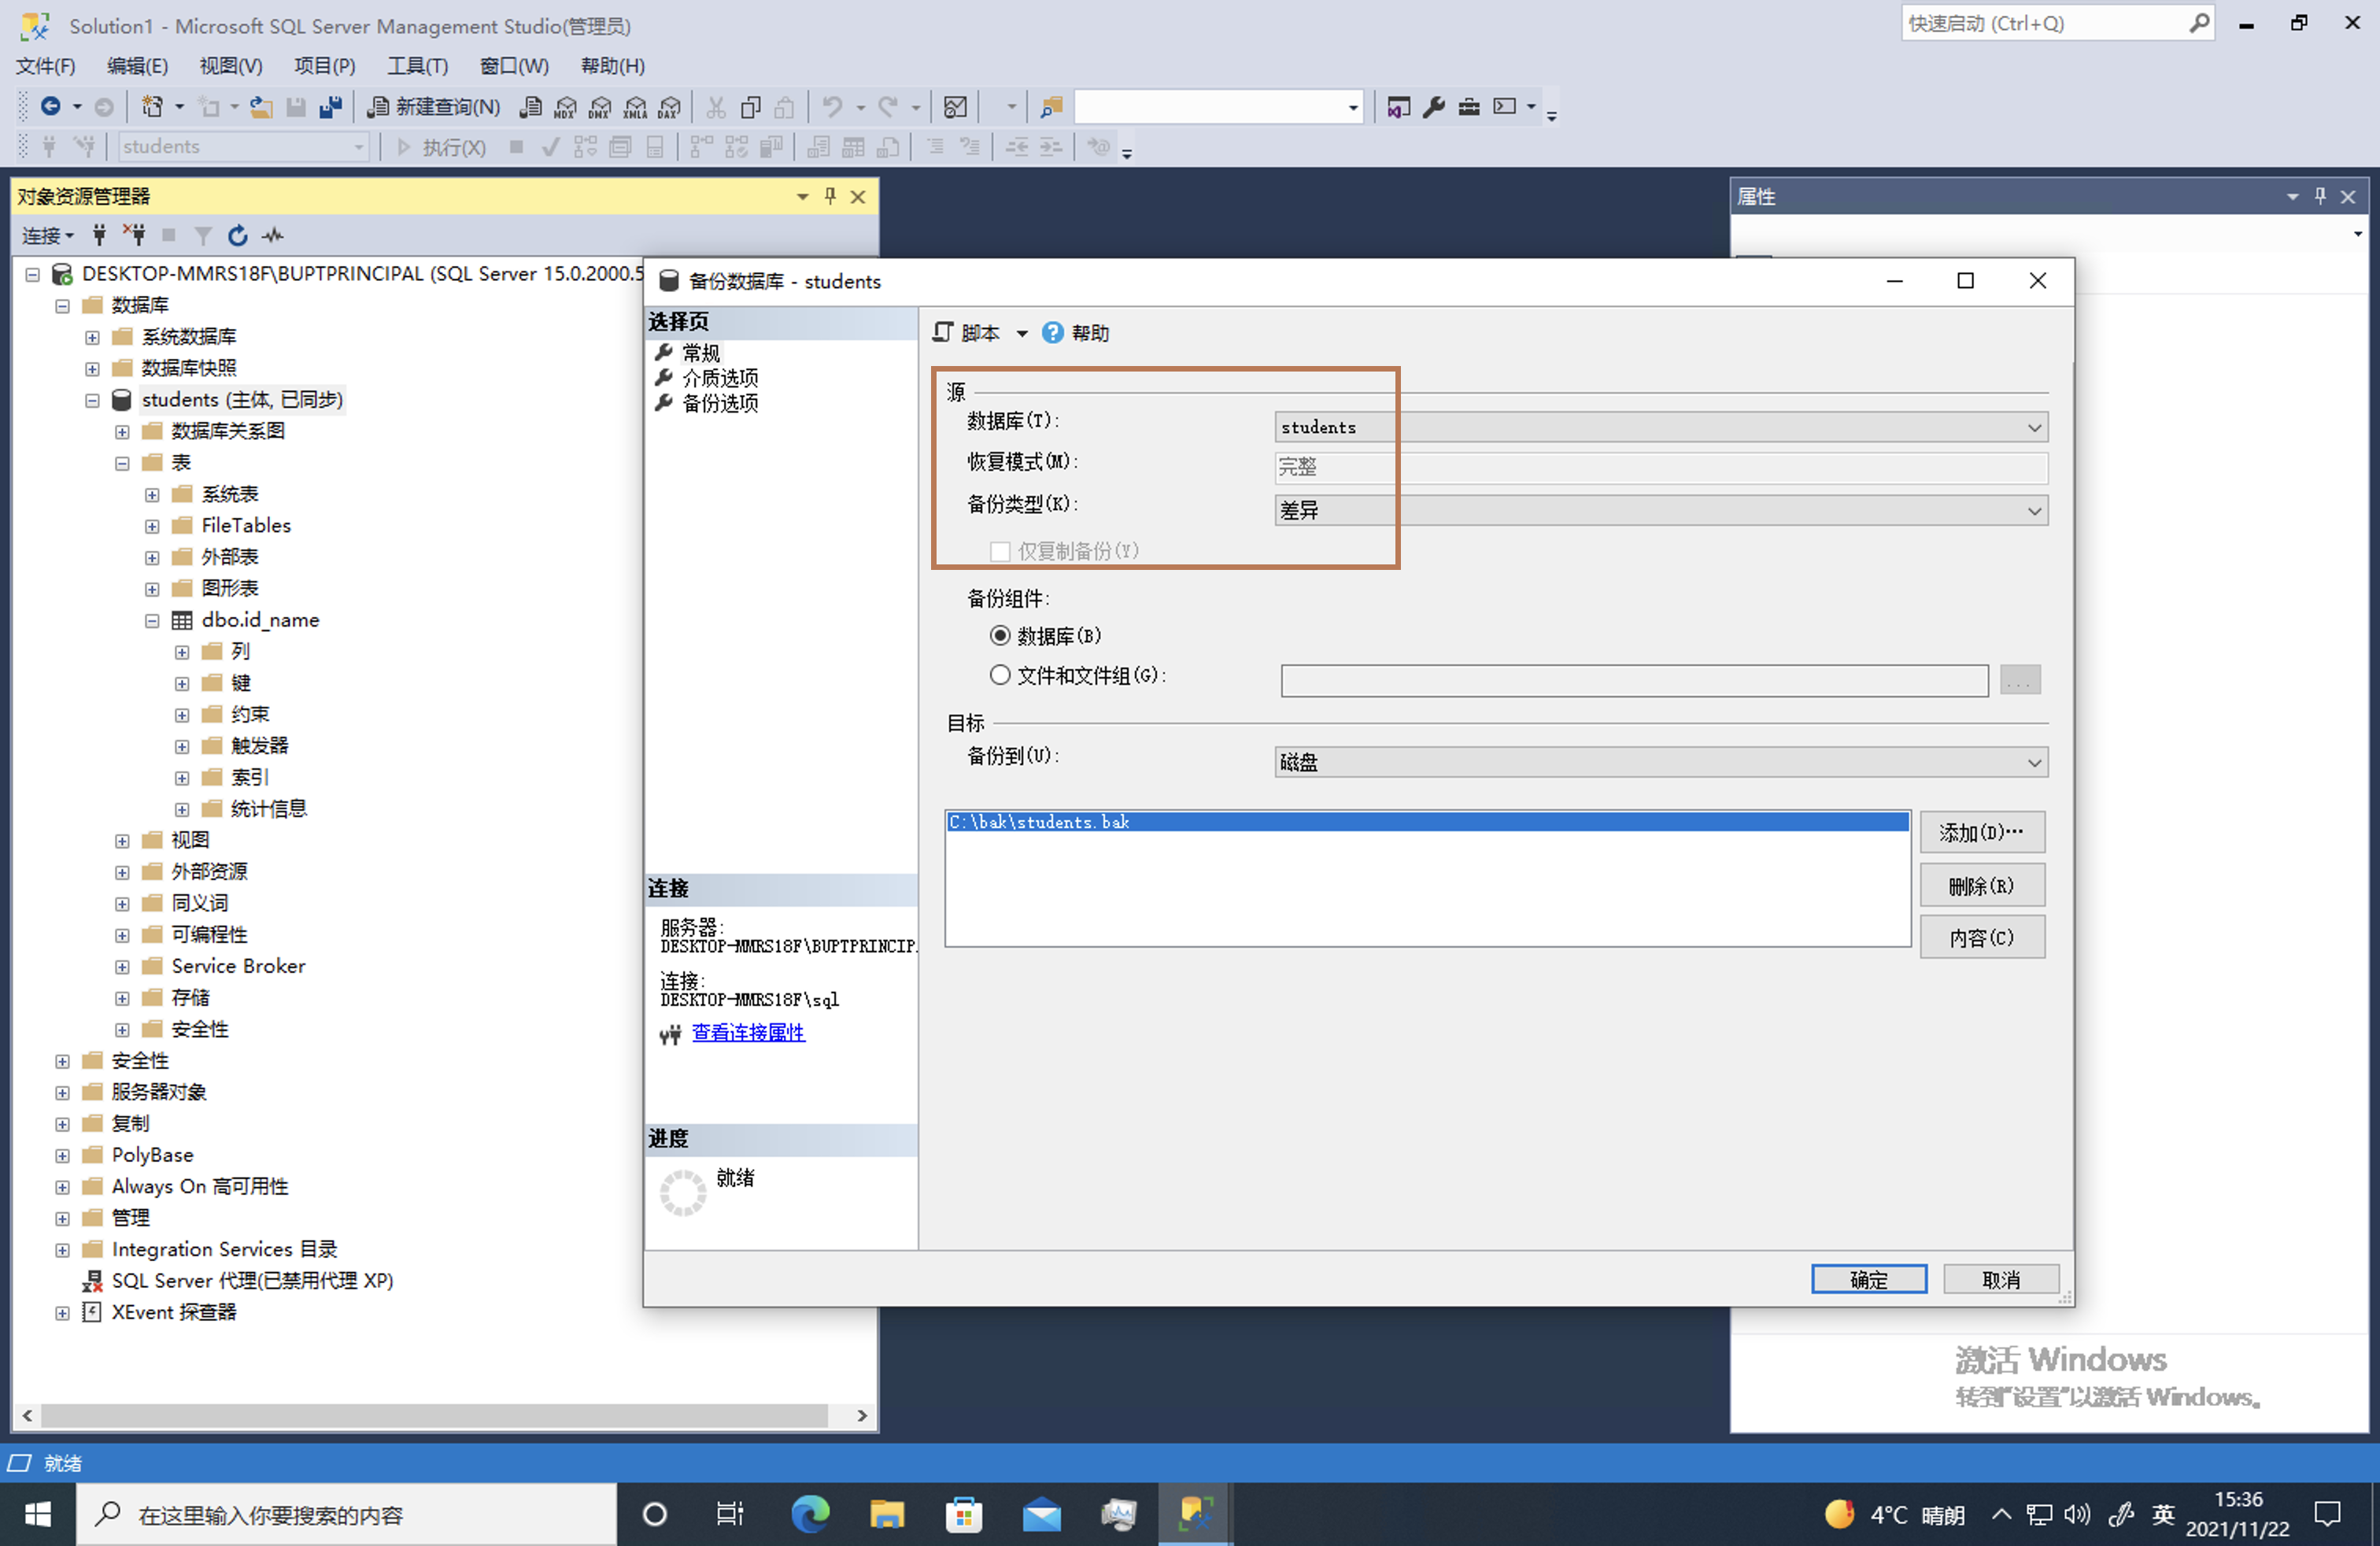
\includegraphics[width=0.70\textwidth]{image/pic5.png}
    \caption{差异备份}
    \label{pic5}
  \end{figure}

  \subsection{实验结果测试}

  在备份数据库中我们可以进行 \textbf{完整} , \textbf{差异} , \textbf{事务日志}。

  在进行备份后,我们可以进行还原。这可以来测试我们的备份是否有效。
  见Figure \ref{pic6}。

  \newpage

  \begin{figure}[h]
    \centering
    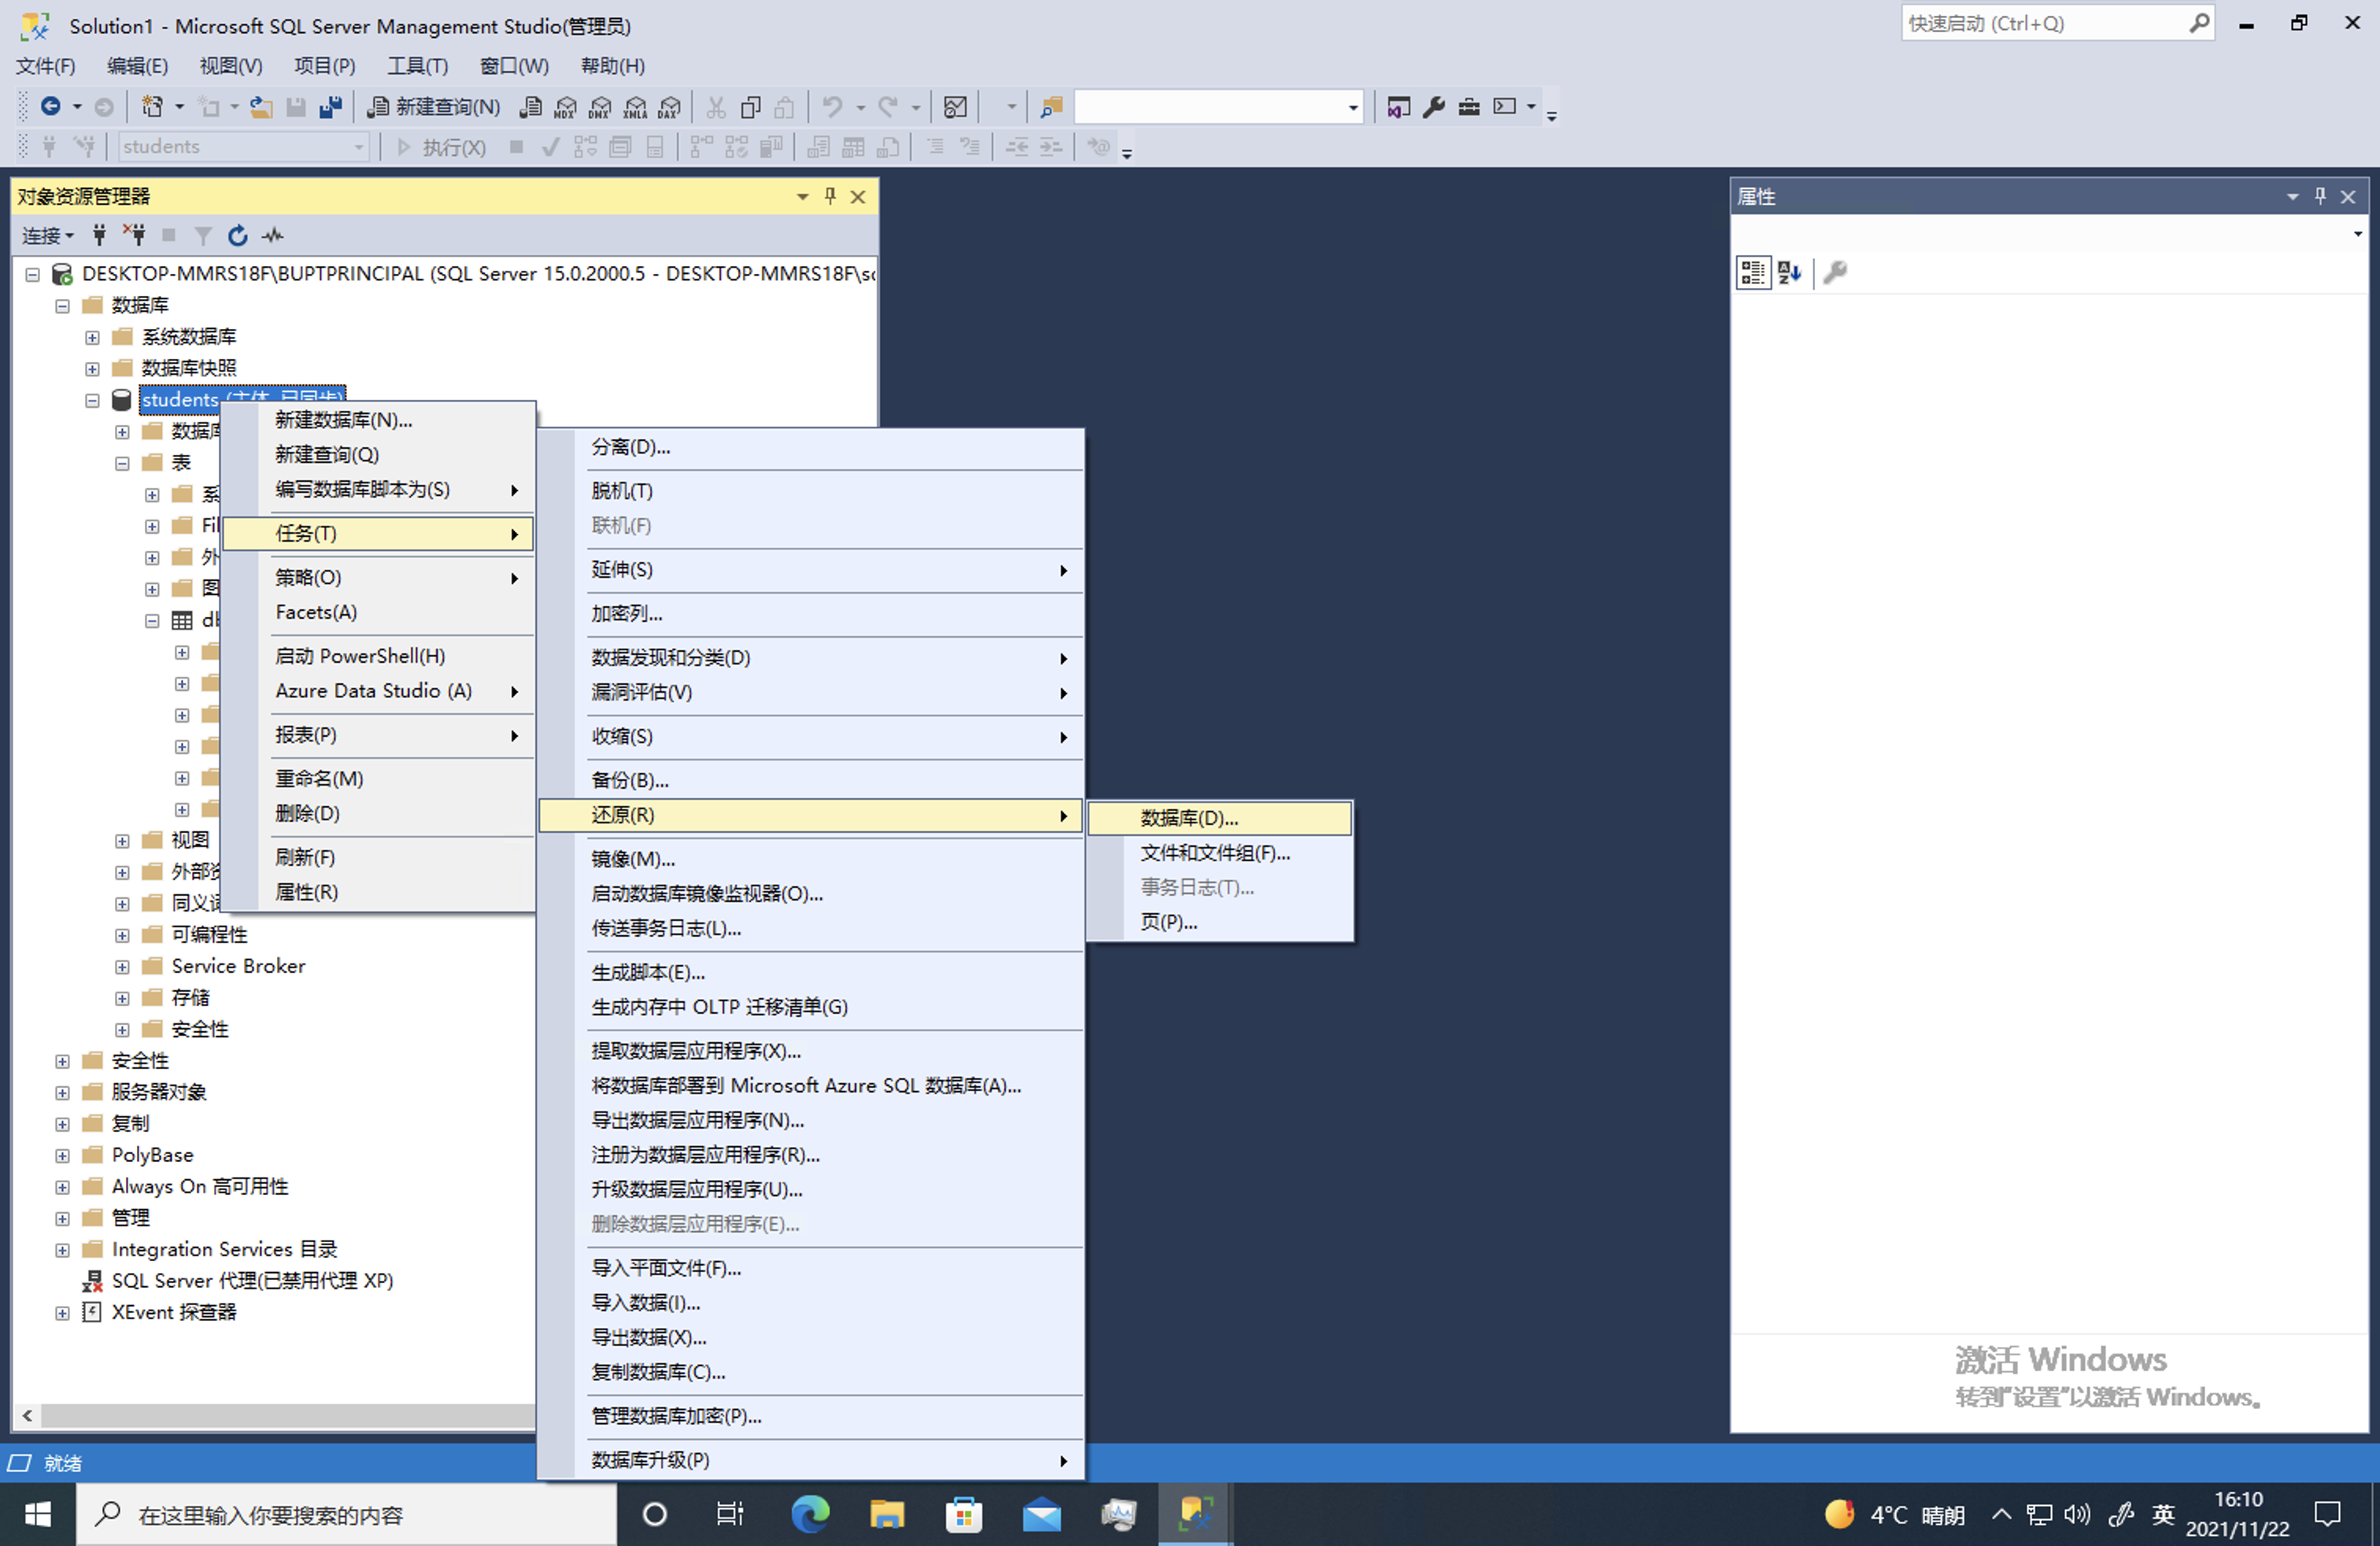
\includegraphics[width=0.70\textwidth]{image/pic6.png}
    \caption{还原数据库}
    \label{pic6}
  \end{figure}

  可以看到,在可以还原的备份集上面,有我们之前的备份的完整备份,差异备份和事物日志。这在后面镜像功能中将会使用。
  见Figure \ref{pic7}。

  \begin{figure}[h]
    \centering
    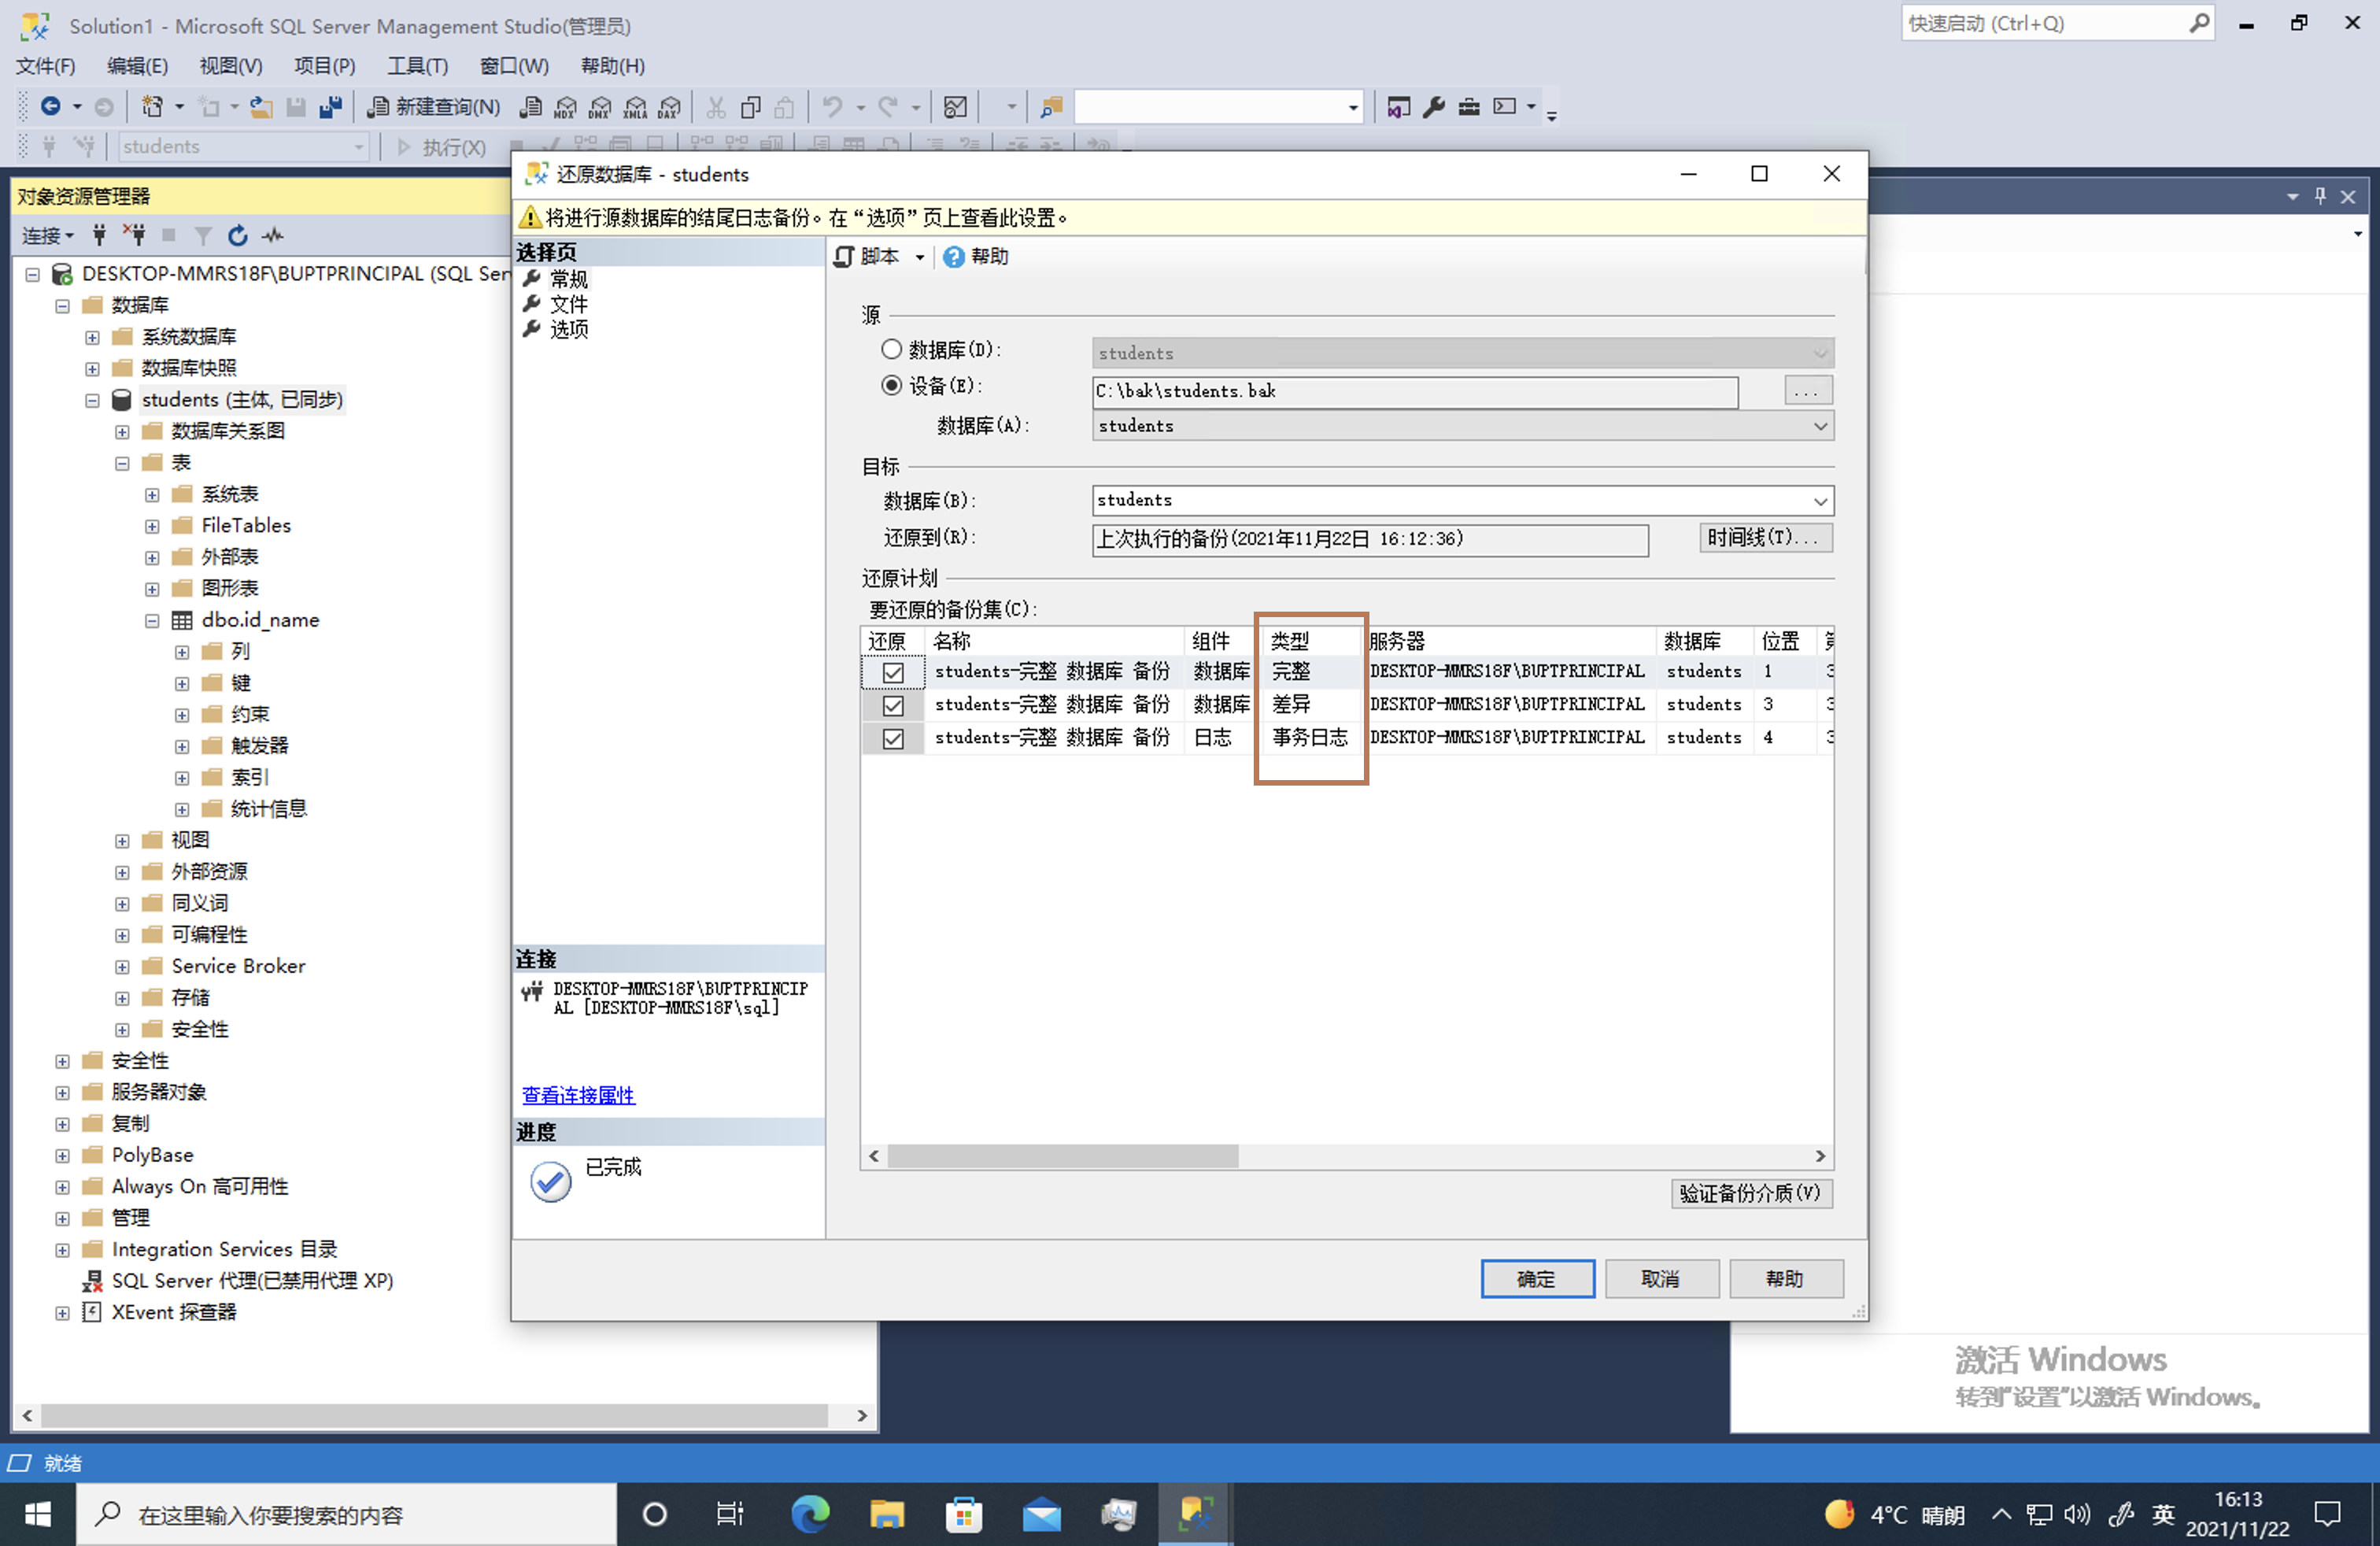
\includegraphics[width=0.70\textwidth]{image/pic7.png}
    \caption{还原数据库}
    \label{pic7}
  \end{figure}

  \section{镜像}

  “数据库镜像” 是一种提高 SQL Server 数据库的可用性的解决方案。
  镜像基于每个数据库实现,并且只适用于使用完整恢复模式的数据库。

  \subsection{同步或异步镜像}

  \subsubsection{先决条件}

  \begin{itemize}
    \item 若要建立镜像会话,伙伴双方和见证服务器(如果有)必须在相同版本的 SQL Server上运行。
    \item 数据库必须使用完整恢复模式。
    \item 在镜像服务器上创建镜像数据库时,请确保指定相同数据库名称 WITH NORECOVERY 来还原主体数据库备份。 另外,还必须通过 WITH NORECOVERY 应用在该备份执行后创建的所有日志备份。
  \end{itemize}

  \subsubsection{限制}

  \begin{itemize}
    \item 只能镜像用户数据库。 不能镜像 master、 msdb、 tempdb 或 model 数据库。
    \item 镜像的数据库在数据库镜像会话过程中不能重命名。
    \item 数据库镜像不支持 FILESTREAM。 不能在主体服务器上创建 FILESTREAM 文件组。 不能为包含 FILESTREAM 文件组的数据库配置数据库镜像。
    \item 跨数据库事务和分布式事务均不支持数据库镜像。
  \end{itemize}

  \subsubsection{镜像状态}

  数据库镜像会话期间,镜像数据库一直处于一种特定状态(镜像状态)。
  数据库的状态反映了通信状态、数据流和伙伴之间数据的差异。
  数据库镜像会话采用的状态与主体数据库相同。

  \subsubsection{操作步骤}

  \begin{enumerate}
    \item 配置镜像服务器,因为我们用单机多数据库服务器,所以使用相同的用户登陆。见Figure \ref{pic8}。
    
    \begin{figure}[h]
      \centering
      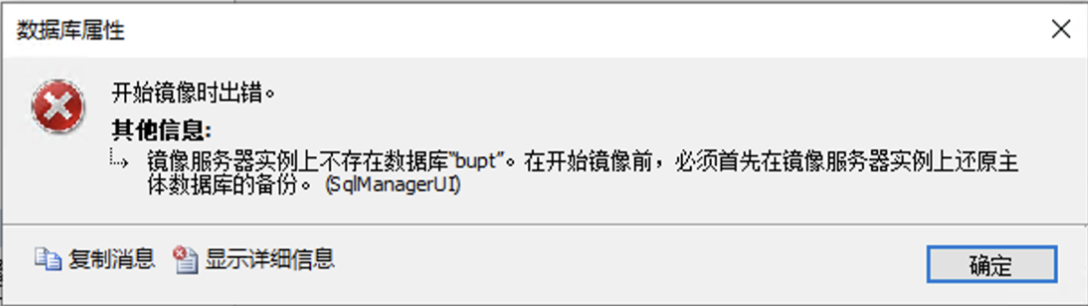
\includegraphics[width=0.70\textwidth]{image/pic8.png}
      \caption{开始镜像前需要先还原}
      \label{pic8}
    \end{figure}

    \item 右键单击数据库,选择 “任务” ,再单击 “镜像” 。 这样便可打开 “数据库属性” 对话框的 “镜像” 页。见Figure \ref{pic9}。
    
    \begin{figure}[h]
      \centering
      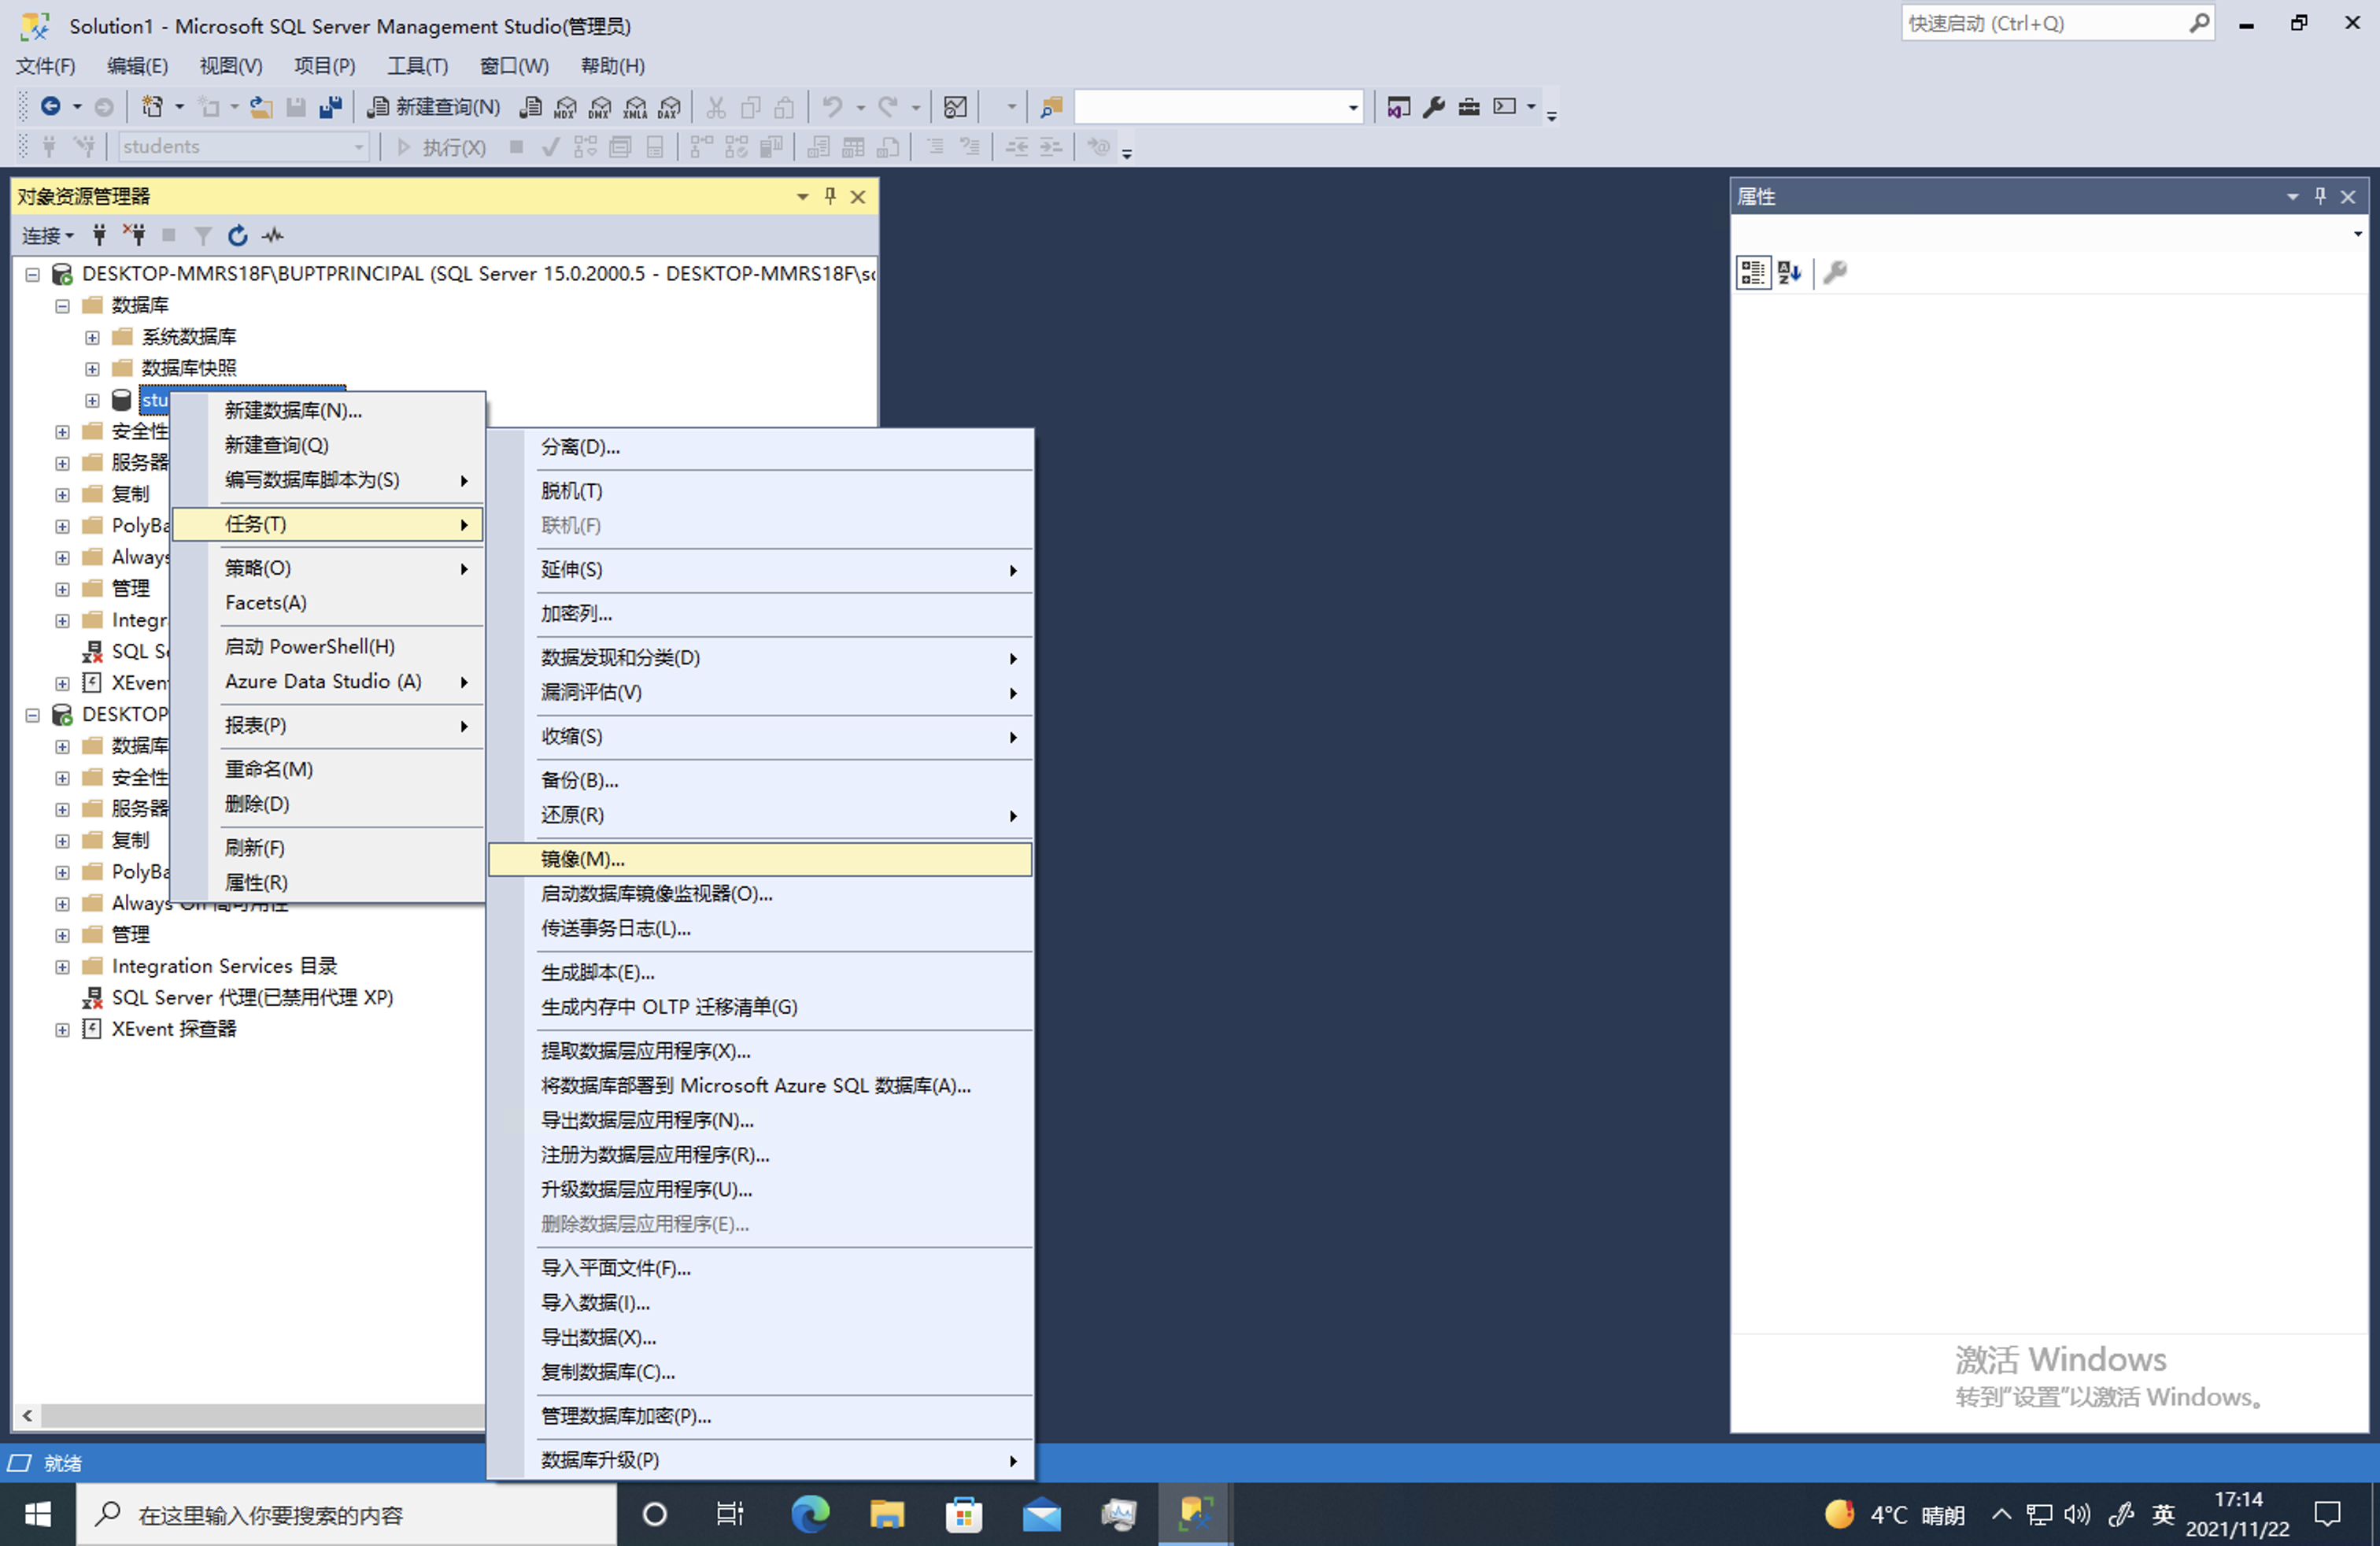
\includegraphics[width=0.70\textwidth]{image/pic9.png}
      \caption{任务->镜像}
      \label{pic9}
    \end{figure}

    \item 若要开始配置镜像,请单击 “配置安全性” 按钮以启动配置数据库镜像安全向导。见Figure \ref{pic10}。
    
    \newpage
    
    \begin{figure}[h]
      \centering
      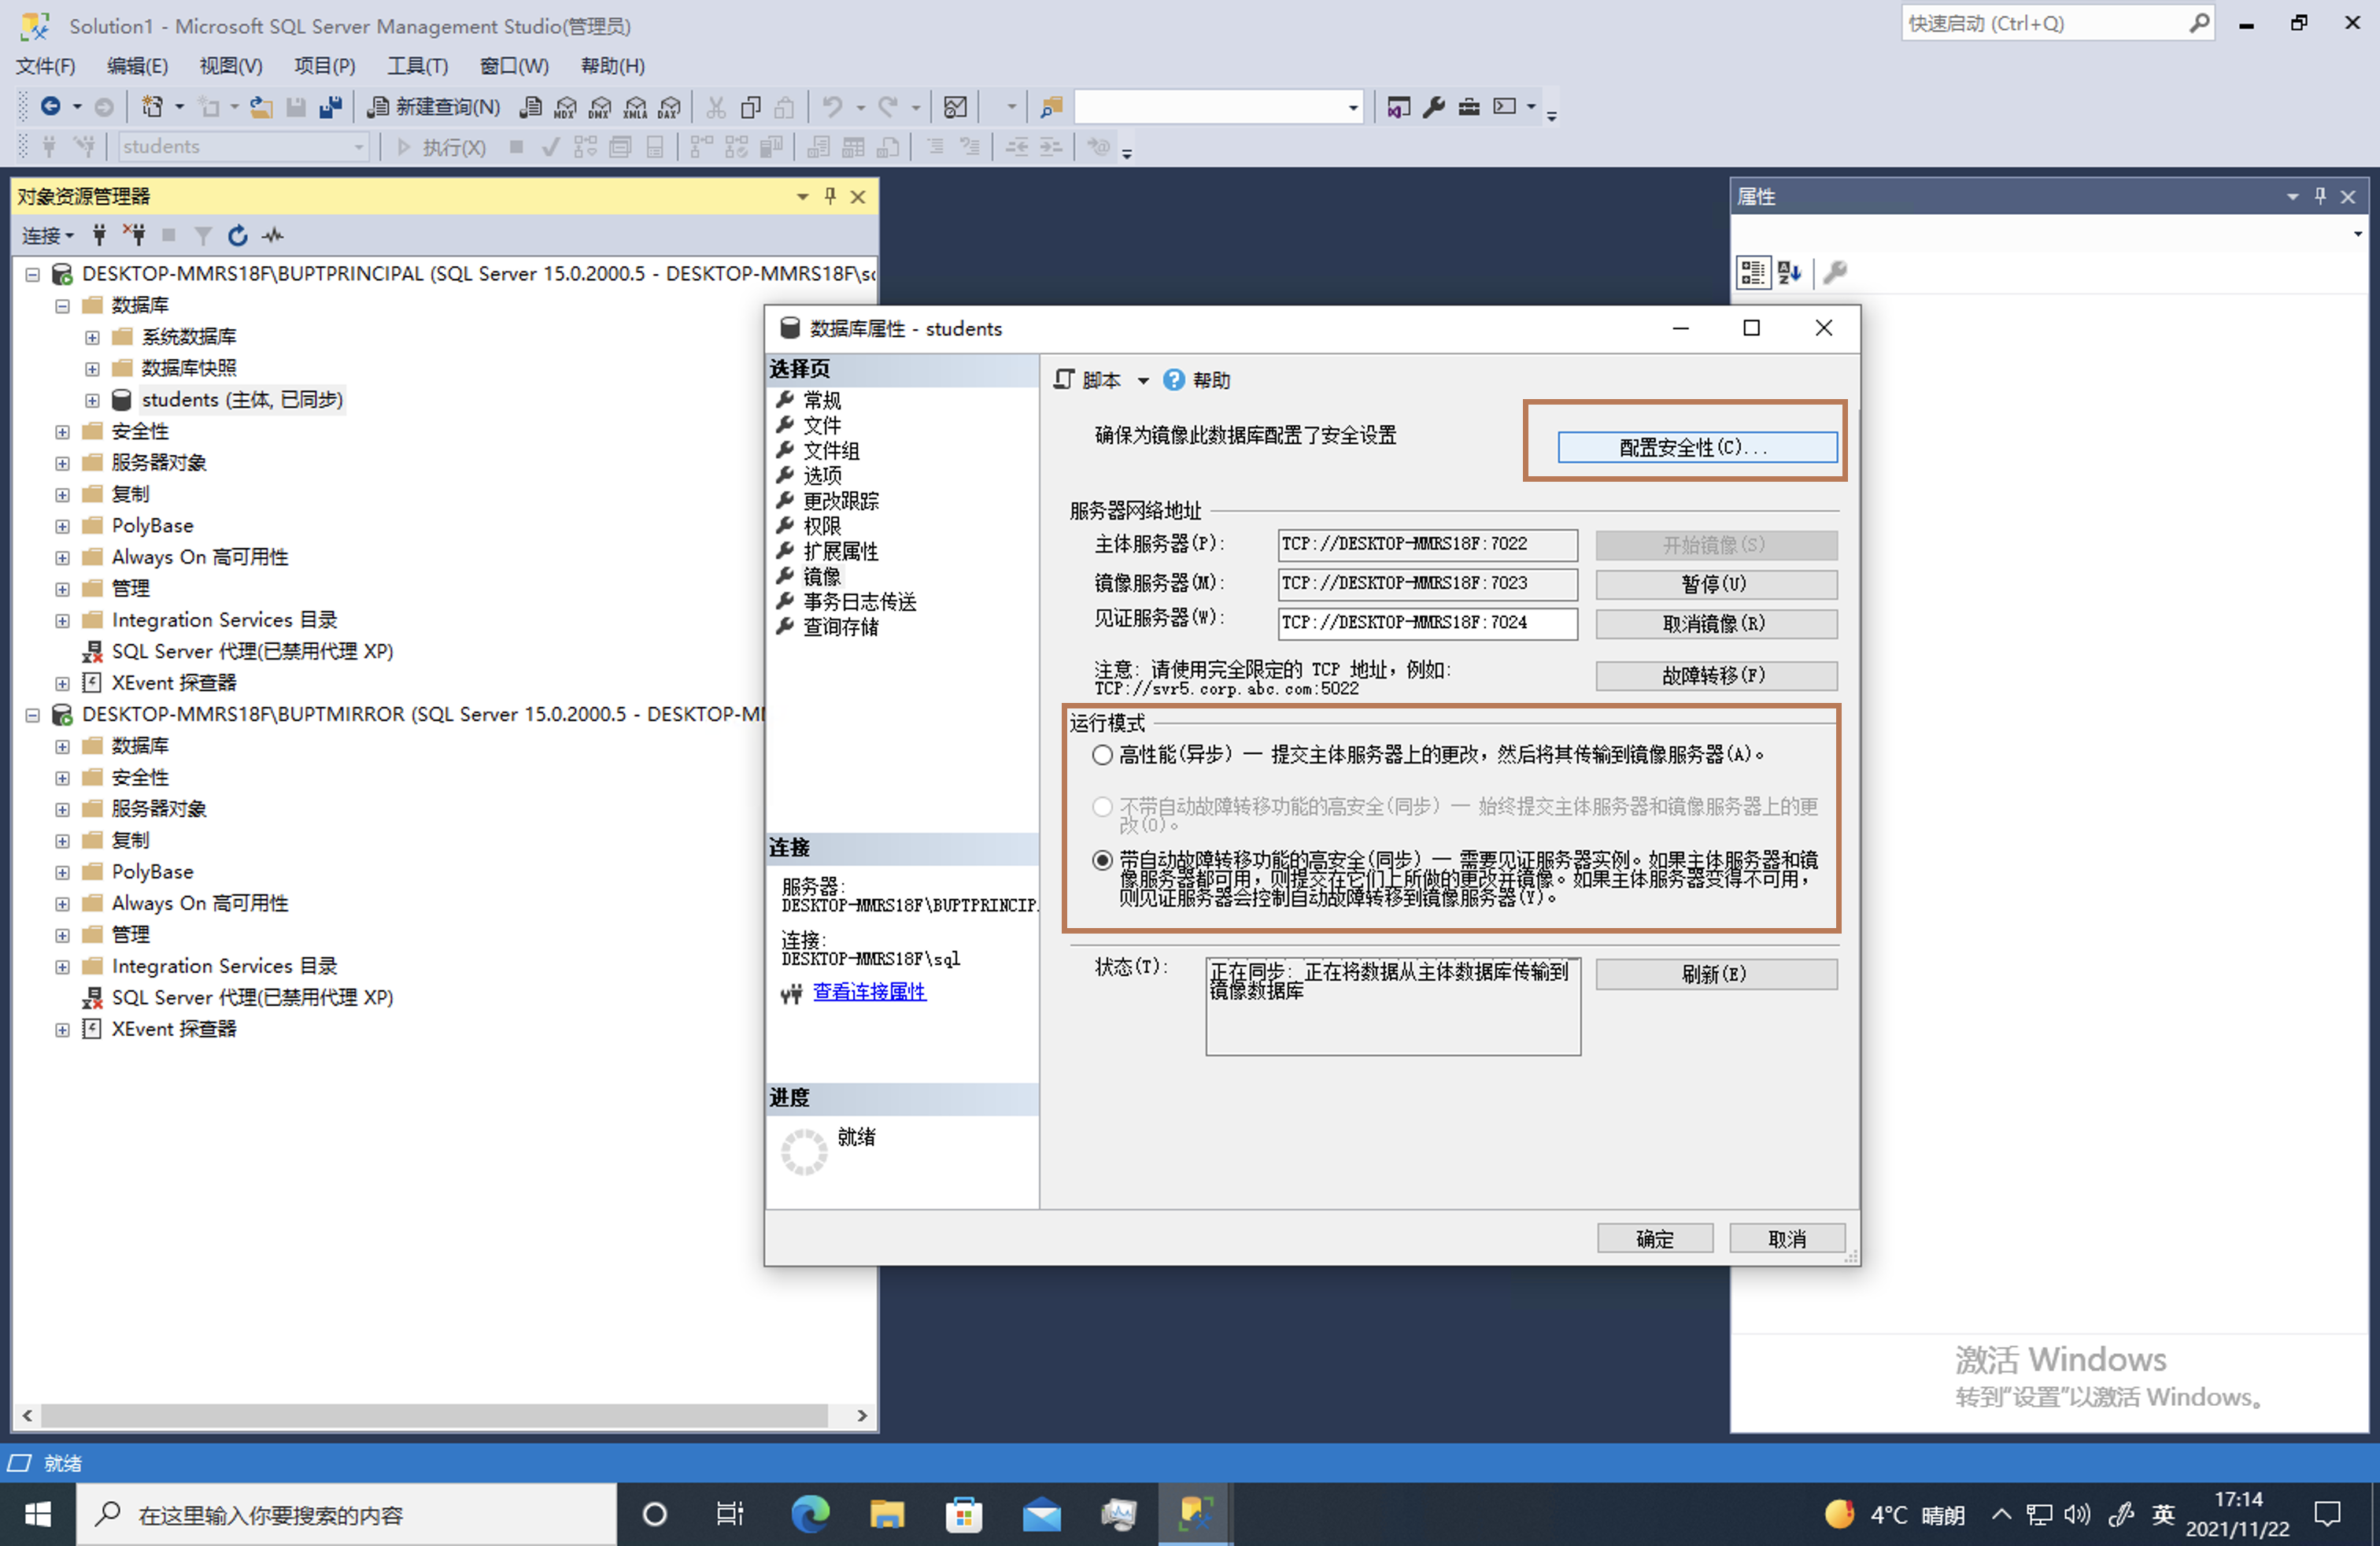
\includegraphics[width=0.70\textwidth]{image/pic10.png}
      \caption{配置安全性}
      \label{pic10}
    \end{figure}

    \item 配置数据库镜像安全向导将在每个服务器实例上自动创建数据库镜像端点(如果不存在任何端点),并在与服务器实例角色(“主体”、 “镜像服务器” 或 “见证服务器”)相对应的字段中输入服务器网络地址。

    异步镜像+主体服务器+镜像服务器 见Figure \ref{pic11}。

    \begin{figure}[h]
      \centering
      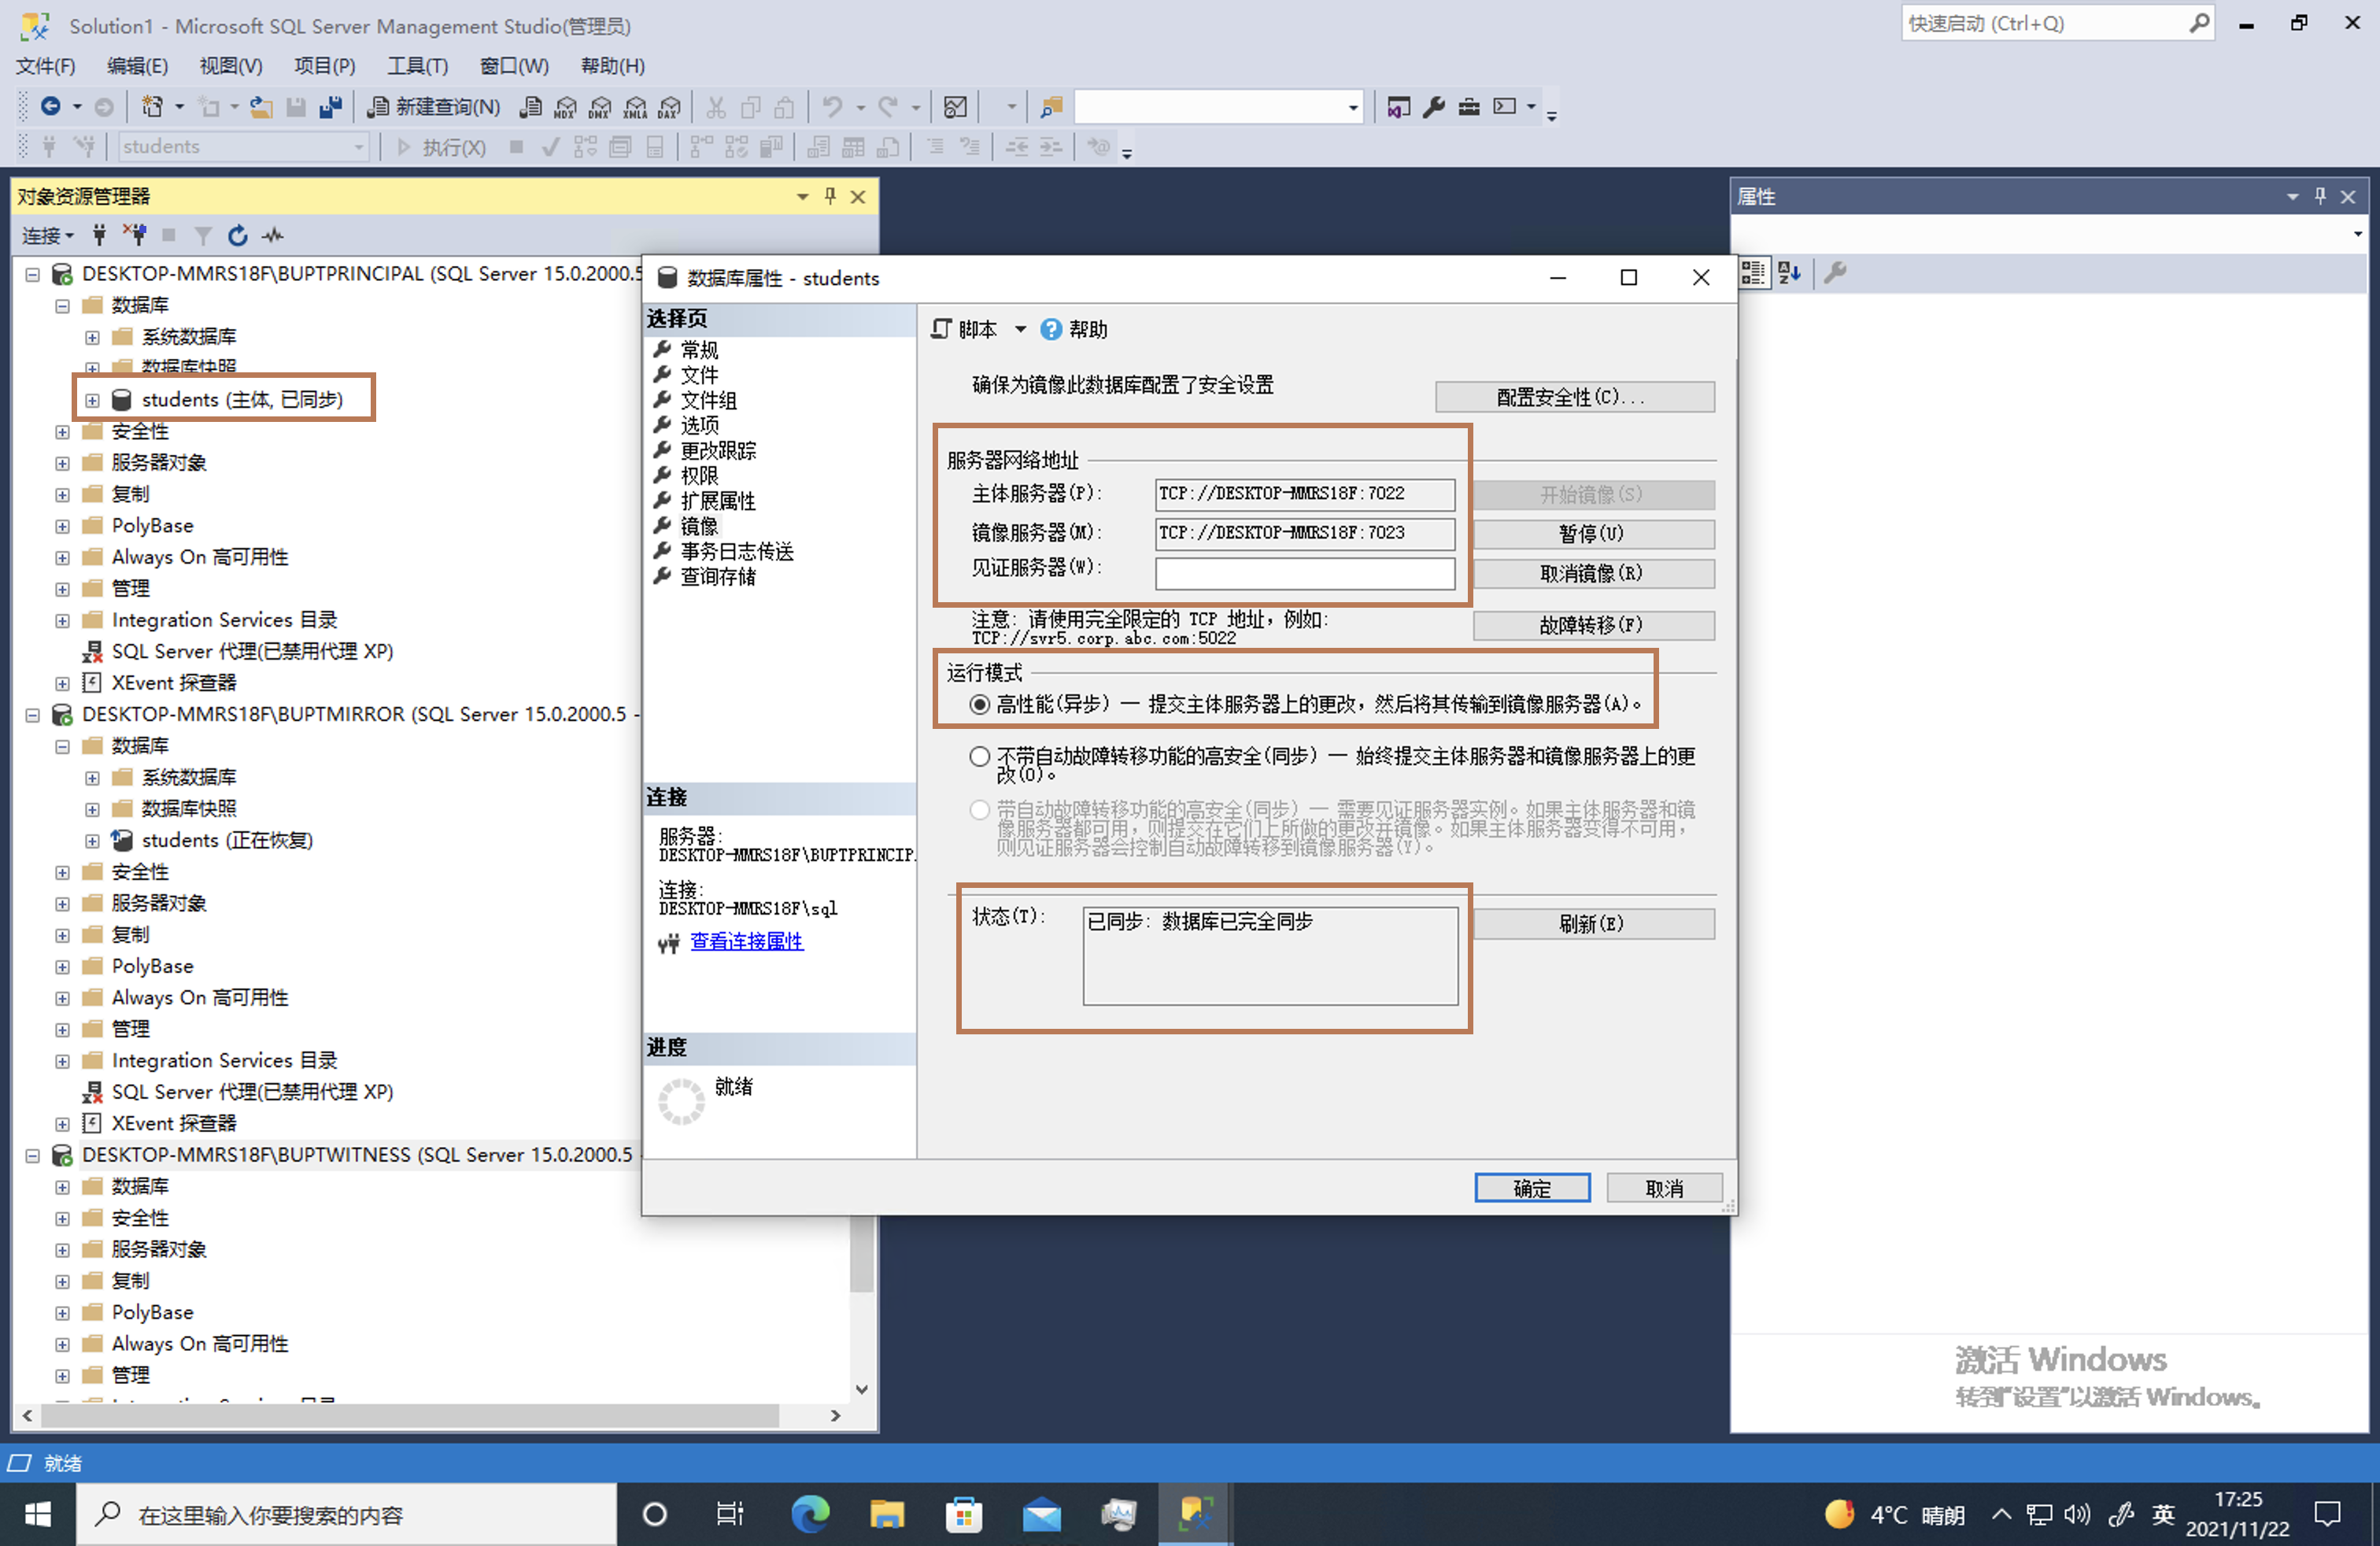
\includegraphics[width=0.70\textwidth]{image/pic11.png}
      \caption{异步+主体+镜像}
      \label{pic11}
    \end{figure}

  \end{enumerate}

  \subsection{有见证服务器}

  若要支持自动故障转移,必须在高安全性模式下配置数据库镜像会话,并且还要具有第三个服务器实例(也称为“见证服务器”)。
  见证服务器是 SQL Server 的可选实例,它能使高安全性模式会话中的镜像服务器识别出是否要启动自动故障转移。
  与这两个伙伴不同的是,见证服务器并不能用于数据库。 见证服务器的唯一角色是支持自动故障转移。

  同步镜像+主体服务器+镜像服务器+见证服务器,见Figure \ref{pic12}。

  \newpage

  \begin{figure}[h]
    \centering
    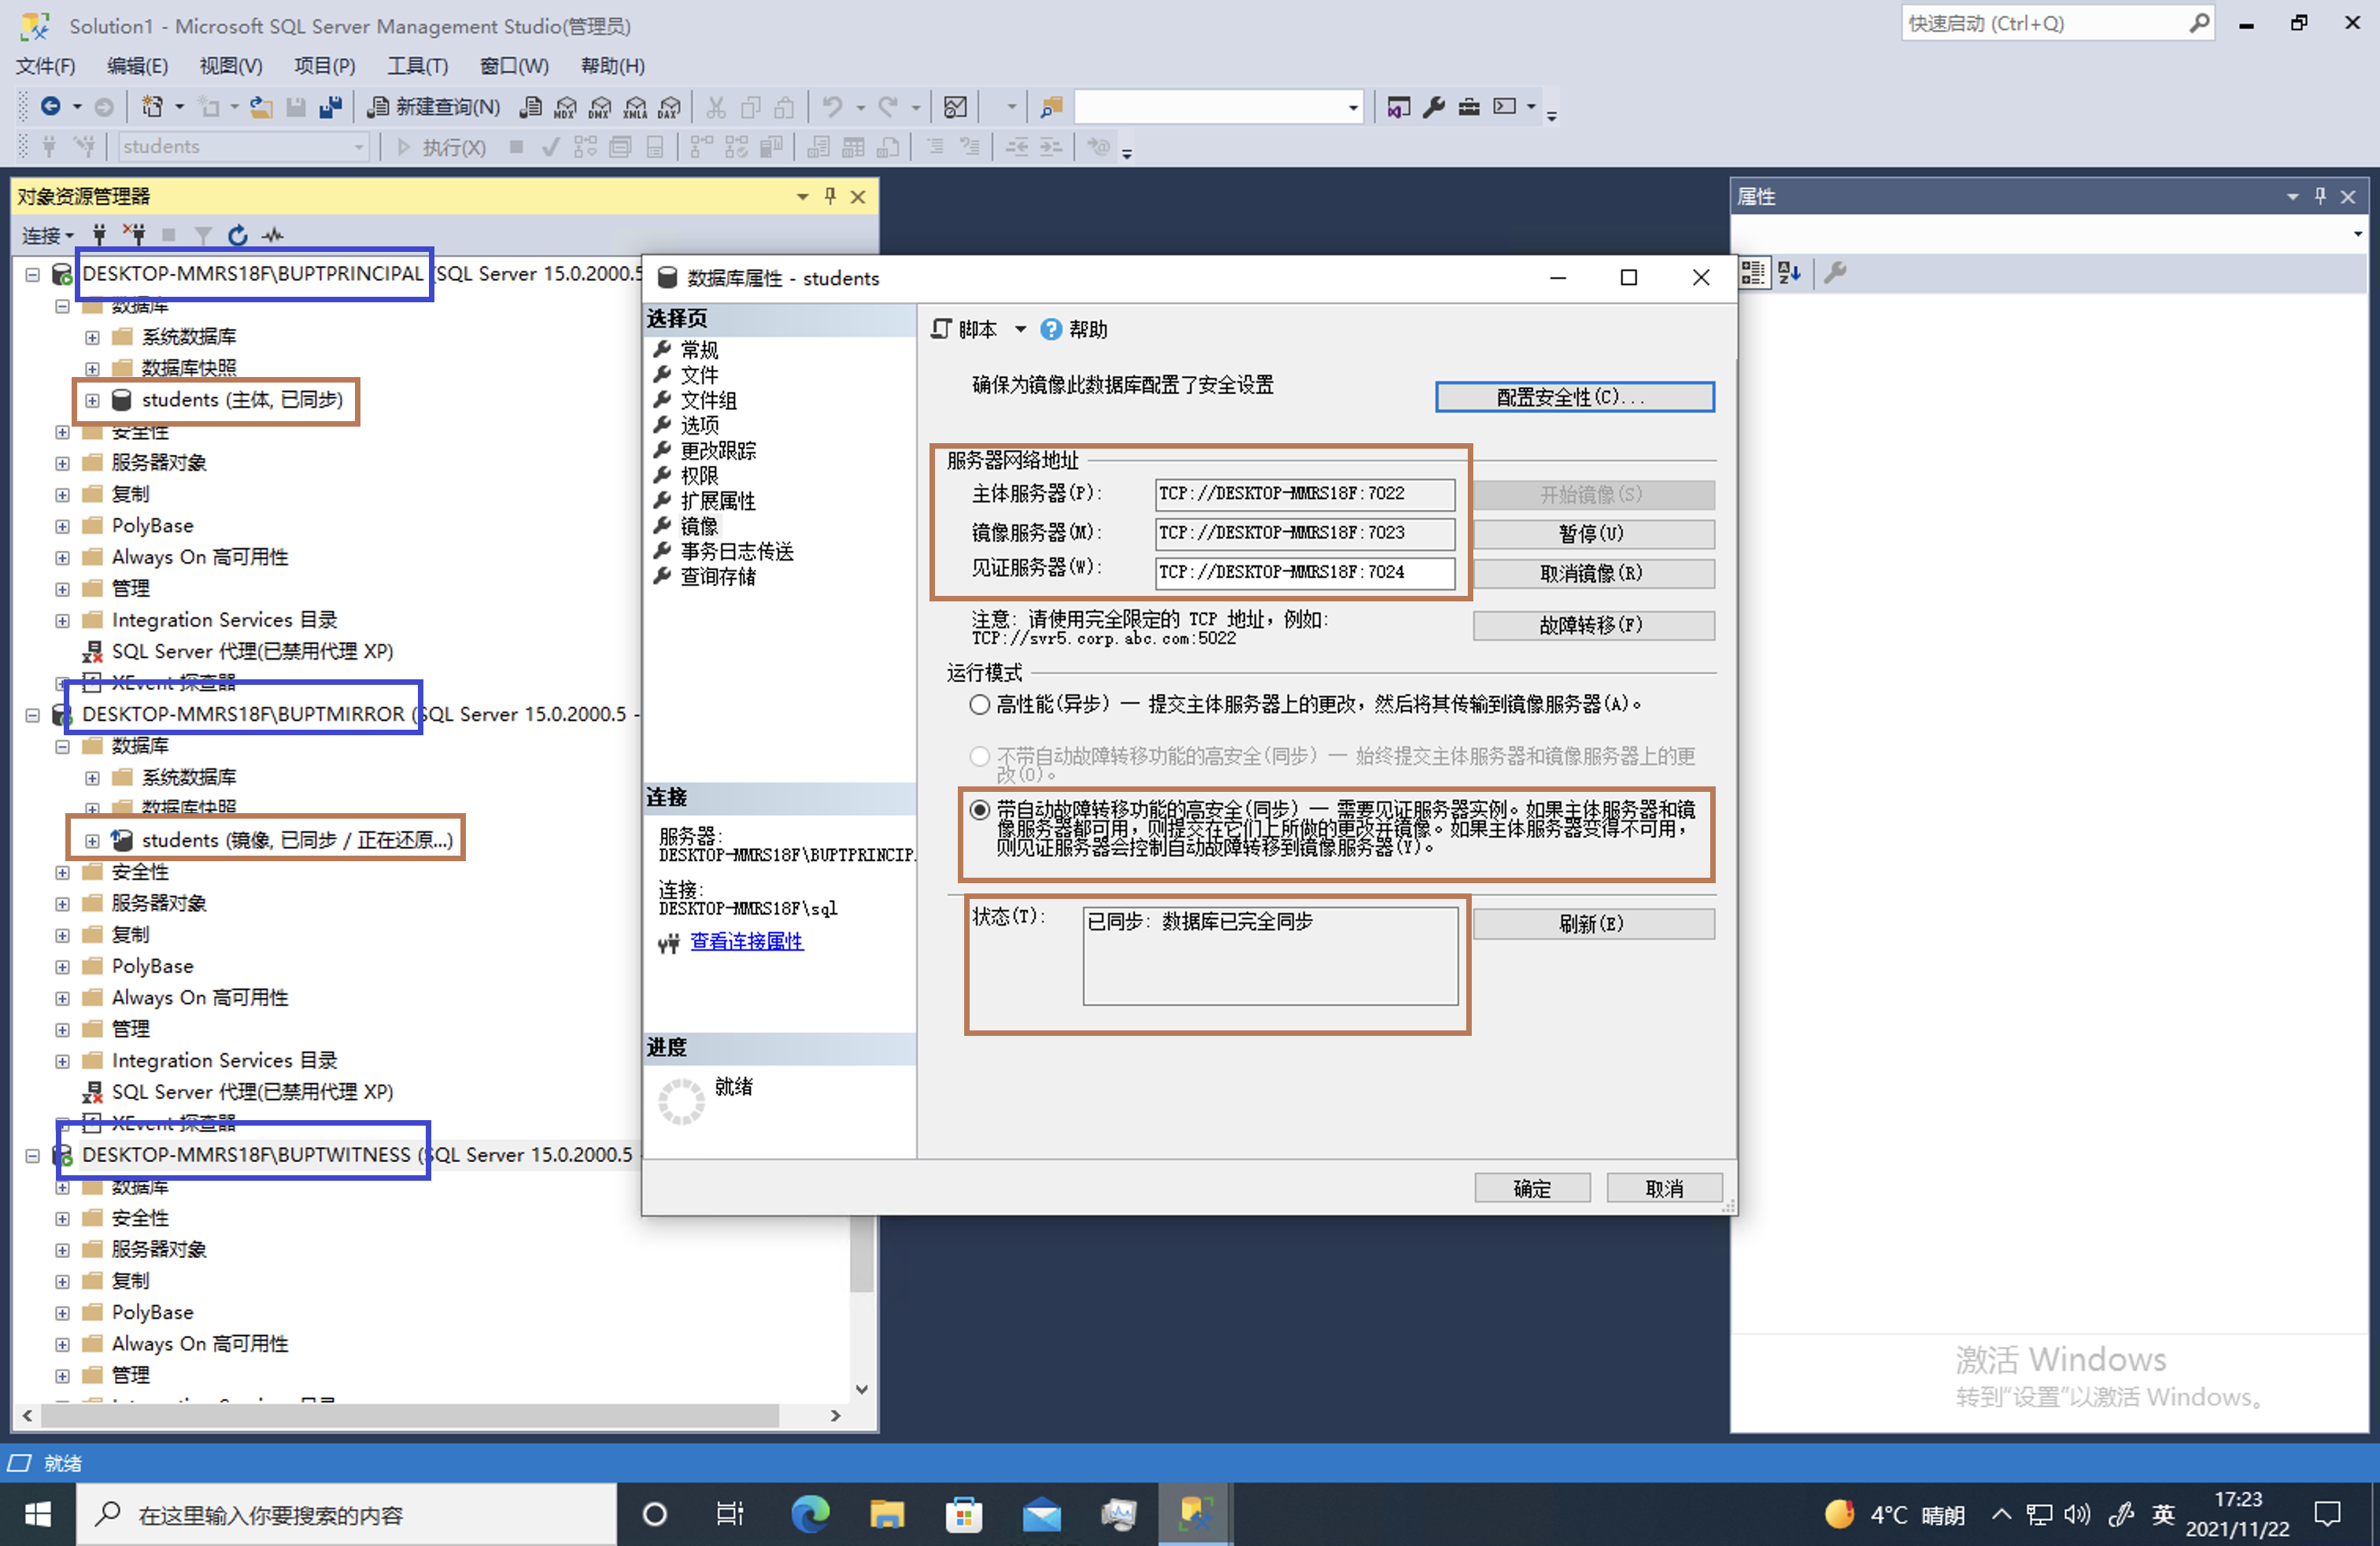
\includegraphics[width=0.70\textwidth]{image/pic12.png}
    \caption{同步+主体+镜像+见证}
    \label{pic12}
  \end{figure}

  \subsection{实验结果测试}

  我们以 \textbf{同步镜像+主体服务器+镜像服务器+见证服务器} 为例做演示。

  \begin{enumerate}

  \item 查看当前主体数据库的表单内容,见Figure \ref{pic13}。

  \begin{figure}[h]
    \centering
    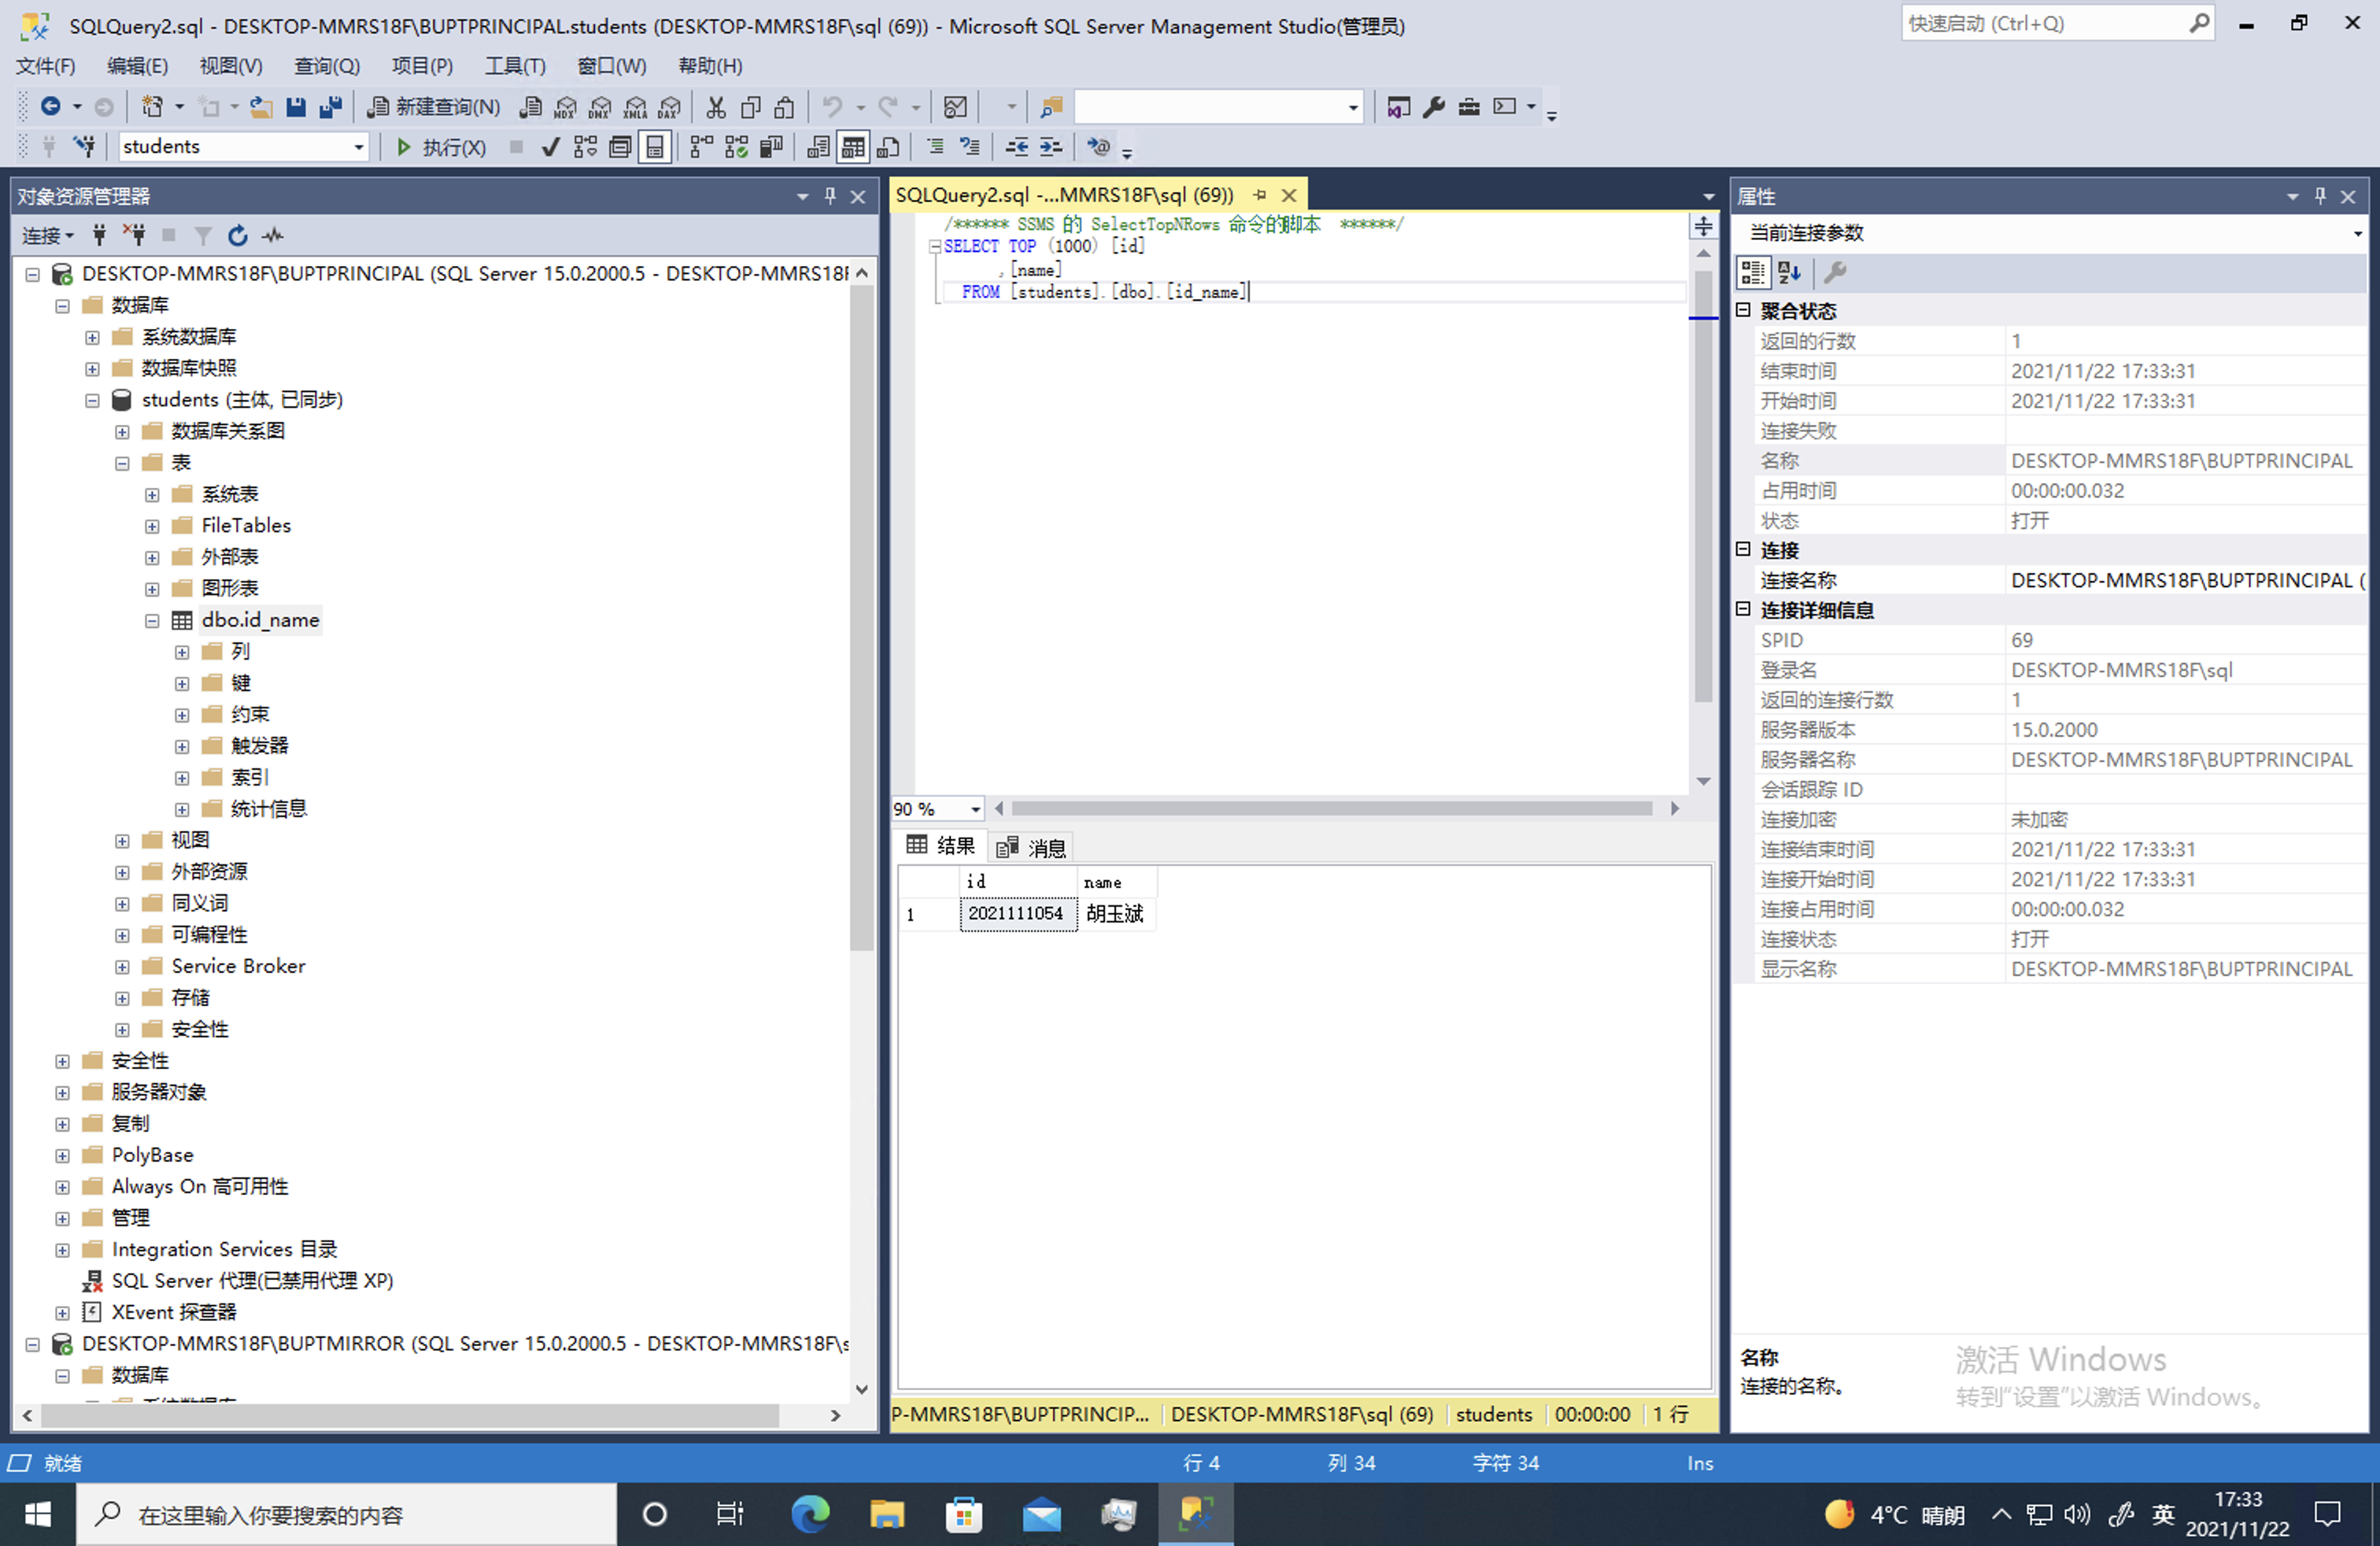
\includegraphics[width=0.70\textwidth]{image/pic13.png}
    \caption{当前主体数据库的表单内容}
    \label{pic13}
  \end{figure}

  \item 修改主体数据库的表单内容,见Figure \ref{pic14}。
  
  \newpage

  \begin{figure}[h]
    \centering
    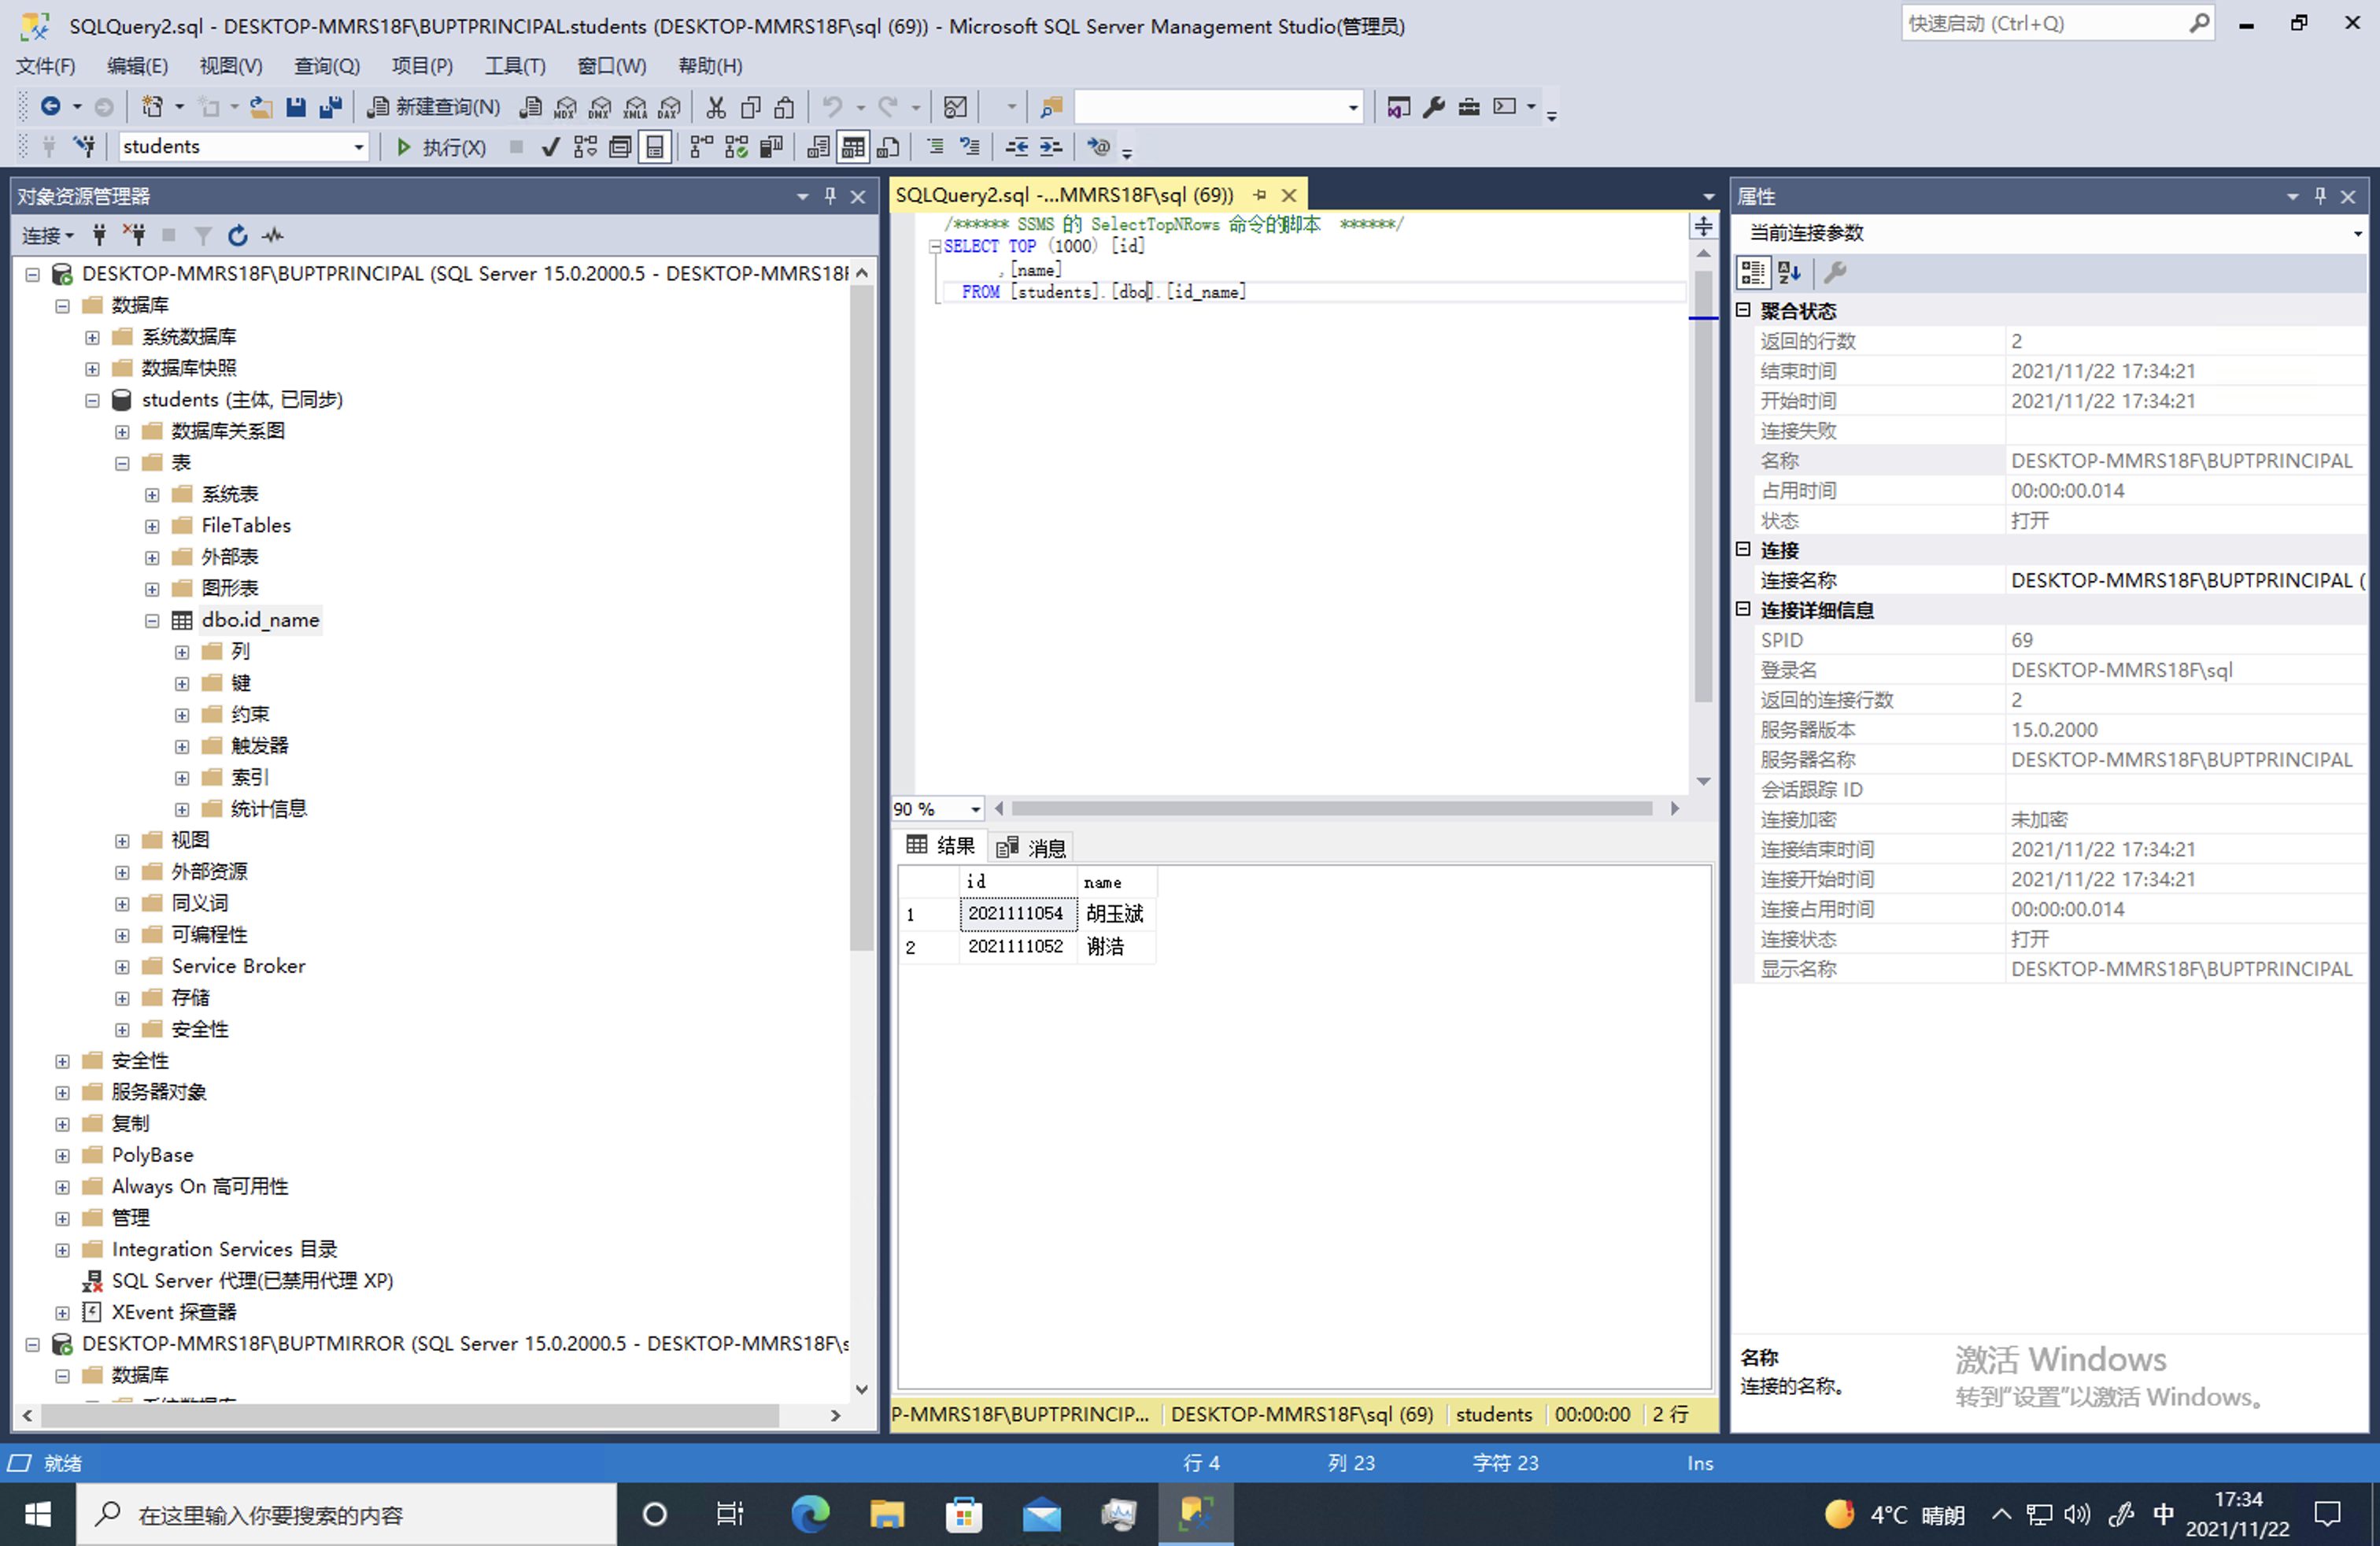
\includegraphics[width=0.70\textwidth]{image/pic14.png}
    \caption{修改后的主体数据库的表单内容}
    \label{pic14}
  \end{figure}

  \item 进行故障转移,模拟主题数据库发生故障,见Figure \ref{pic15}。

  \begin{figure}[h]
    \centering
    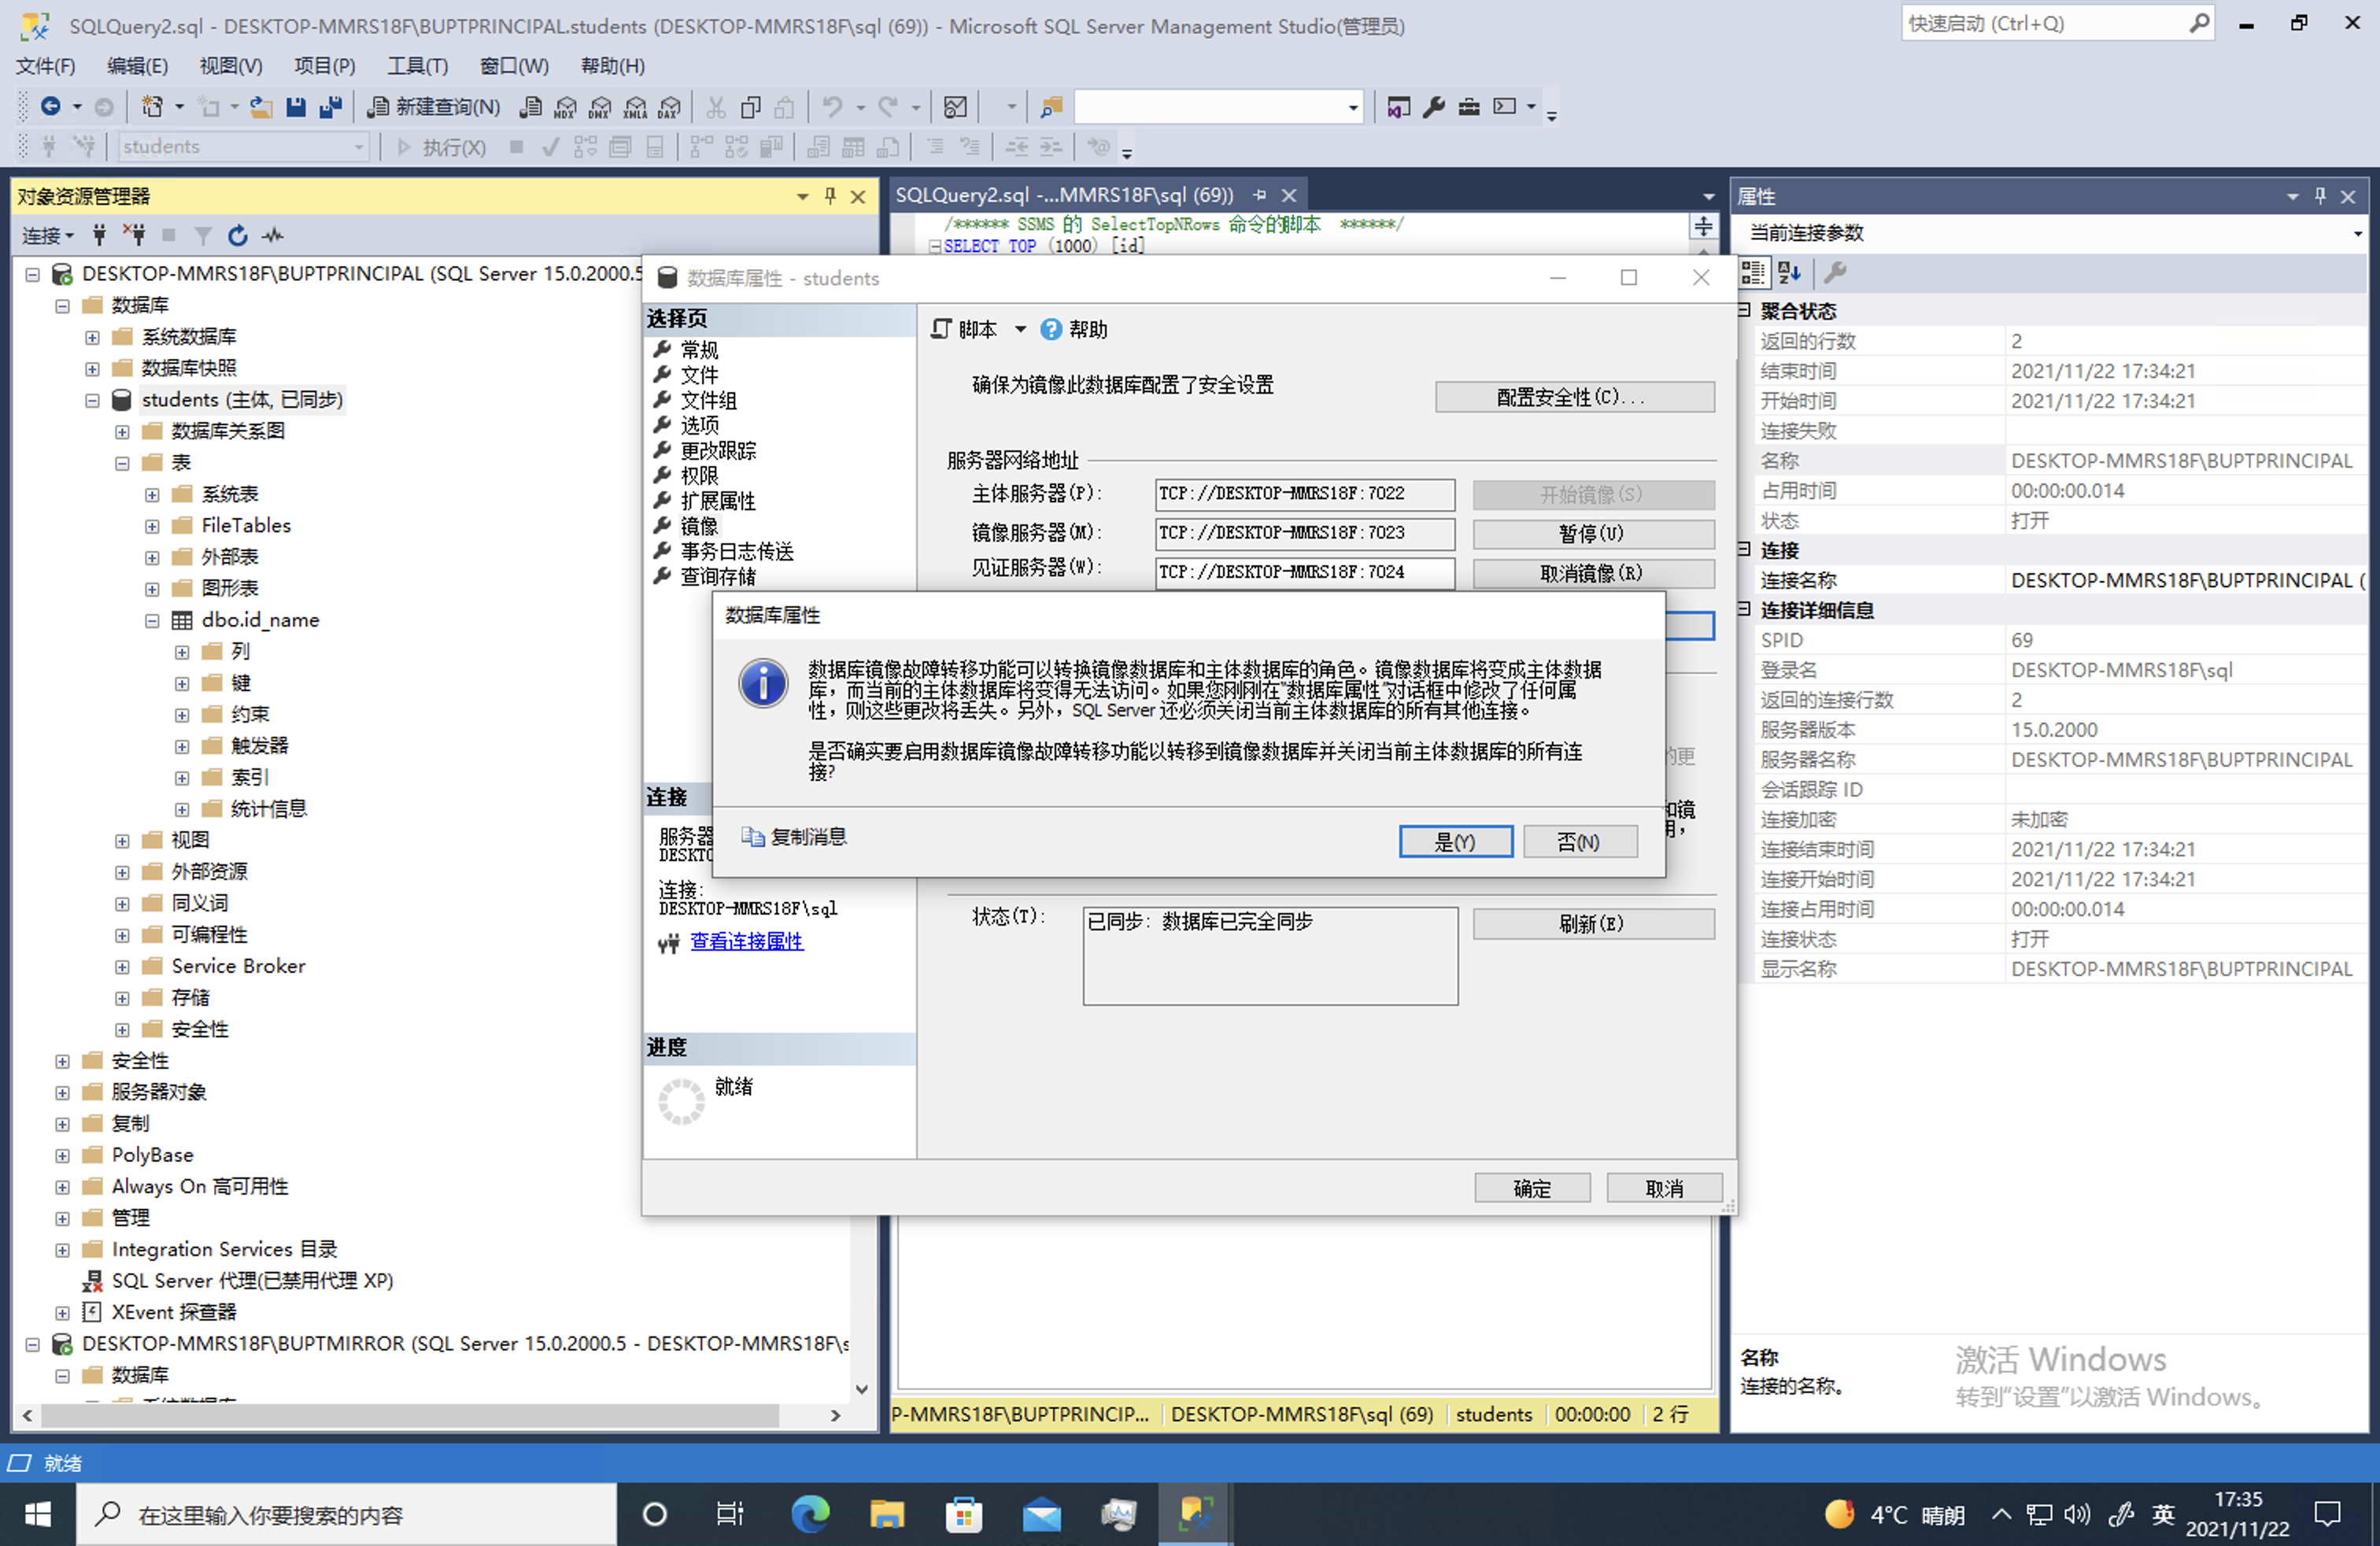
\includegraphics[width=0.70\textwidth]{image/pic15.png}
    \caption{进行故障转移}
    \label{pic15}
  \end{figure}

  \item 主体数据库以及无法访问,查询,见Figure \ref{pic16}。

  \begin{figure}[h]
    \centering
    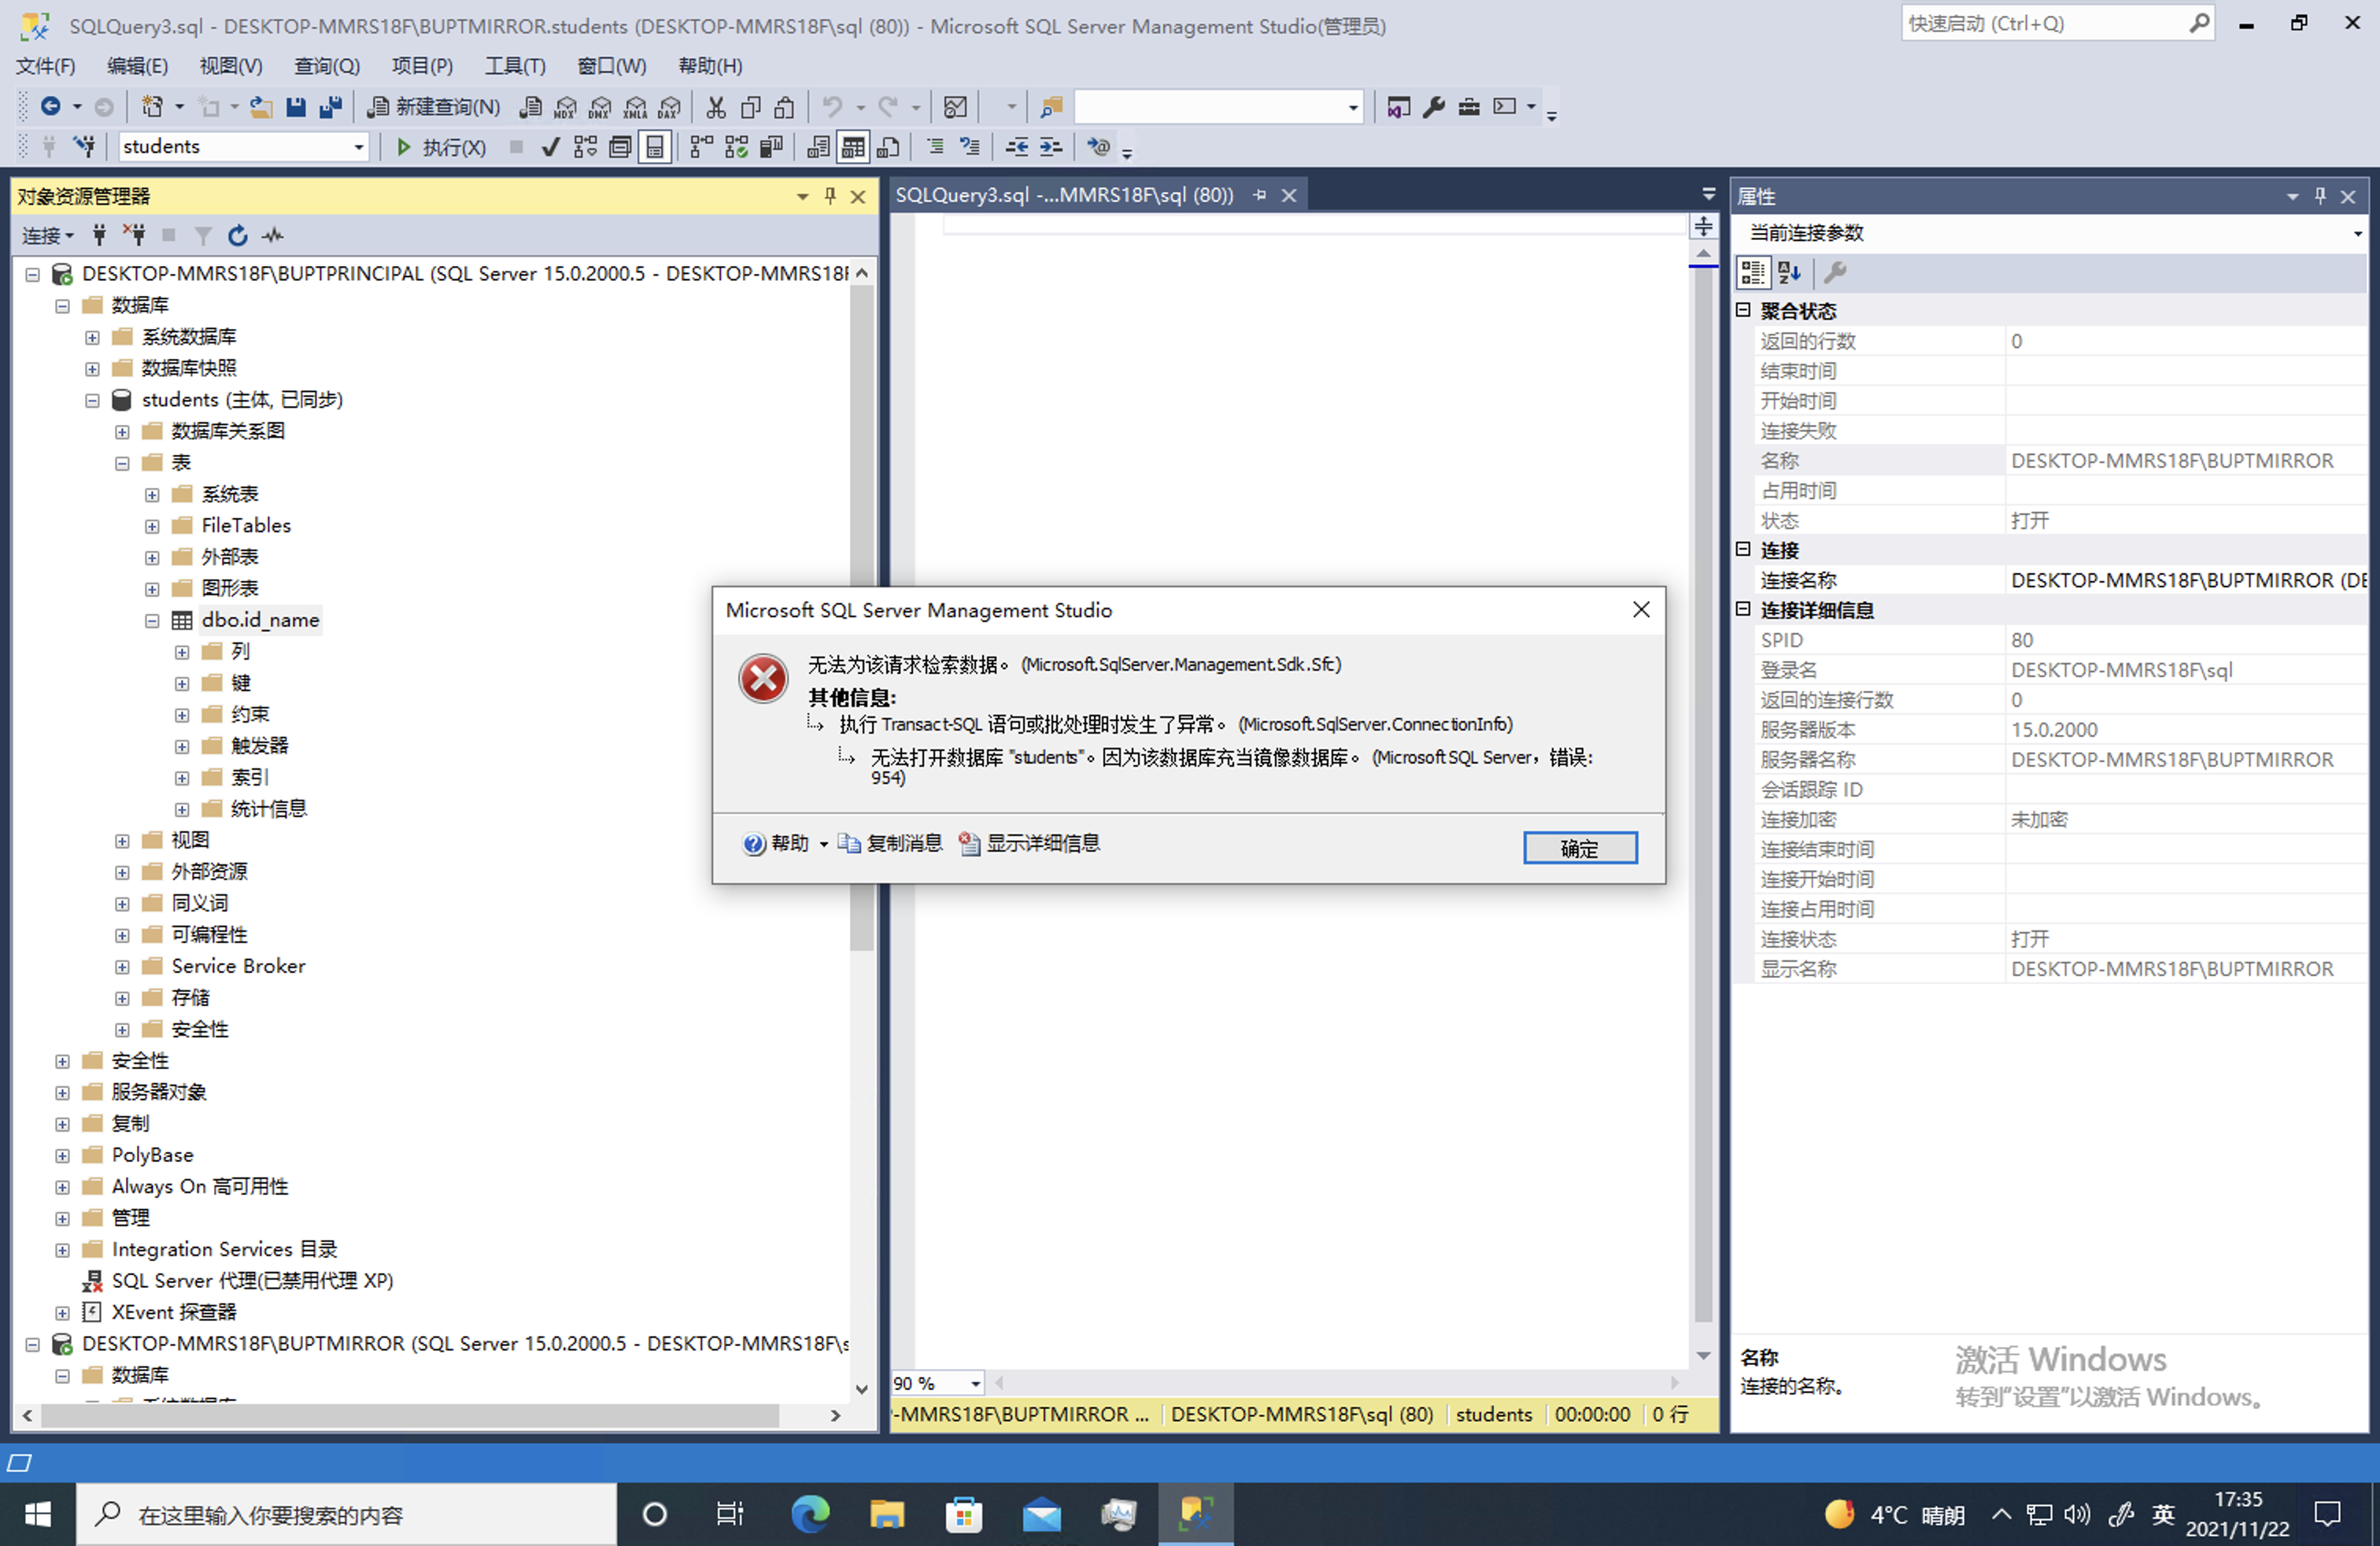
\includegraphics[width=0.70\textwidth]{image/pic16.png}
    \caption{主体数据库以及无法访问,查询}
    \label{pic16}
  \end{figure}

  \newpage

  \item 镜像服务器发挥作用,见证服务器负责见证,见Figure \ref{pic17}。
  
  \begin{figure}[h]
    \centering
    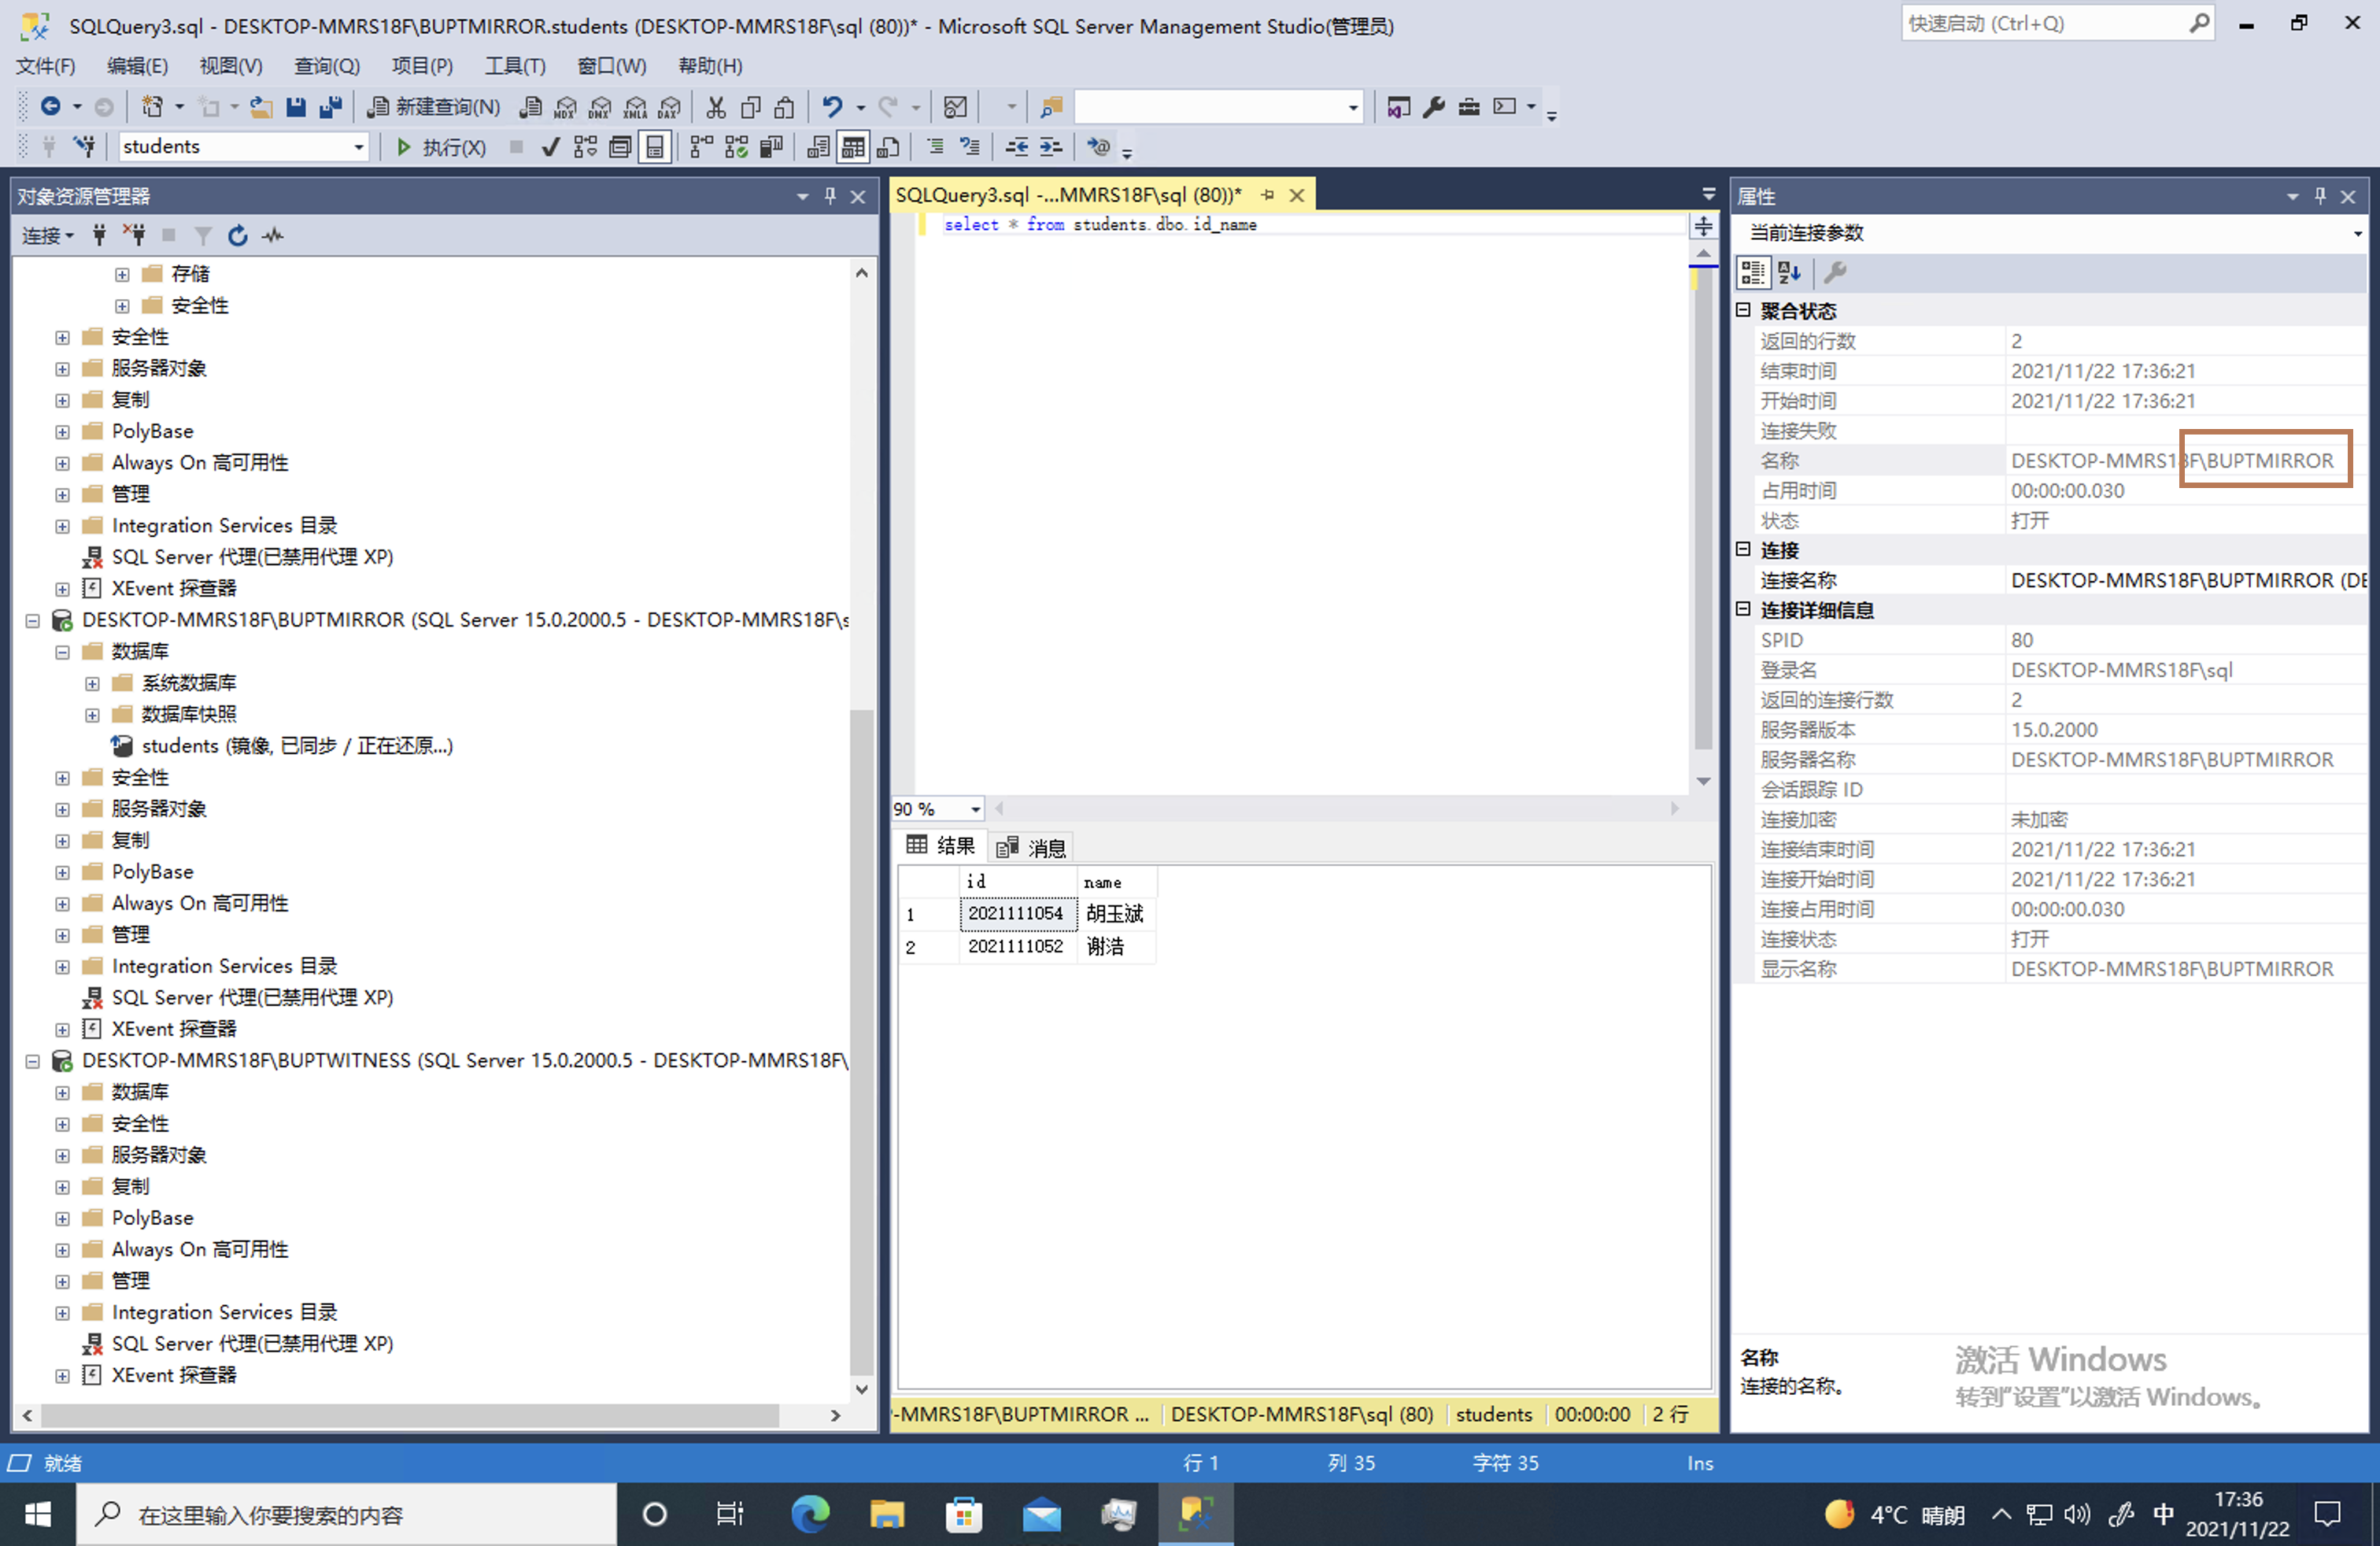
\includegraphics[width=0.70\textwidth]{image/pic17.png}
    \caption{镜像服务器查询结果}
    \label{pic17}
  \end{figure}

  \end{enumerate}

  到这里,可以认为我们的主体+镜像+见证服务器搭建完毕。

  \section{快照}

  SQL Server 文件快照备份使用 Azure 快照提供近乎即时的备份,并且更快速地还原使用 Azure Blob 存储服务存储的数据库文件。
  使用此功能可简化备份和还原策略。

  数据库快照是 SQL Server 数据库(源数据库)的只读静态视图。 
  自创建快照那刻起,数据库快照在事务上与源数据库一致。 
  数据库快照始终与其源数据库位于同一服务器实例上。 

  \subsection{快照创建和查询}

  \begin{enumerate}
    
  \item 本地发布 -> 新建发布,见Figure \ref{pic18}。
  
  \newpage
  
  \begin{figure}[h]
    \centering
    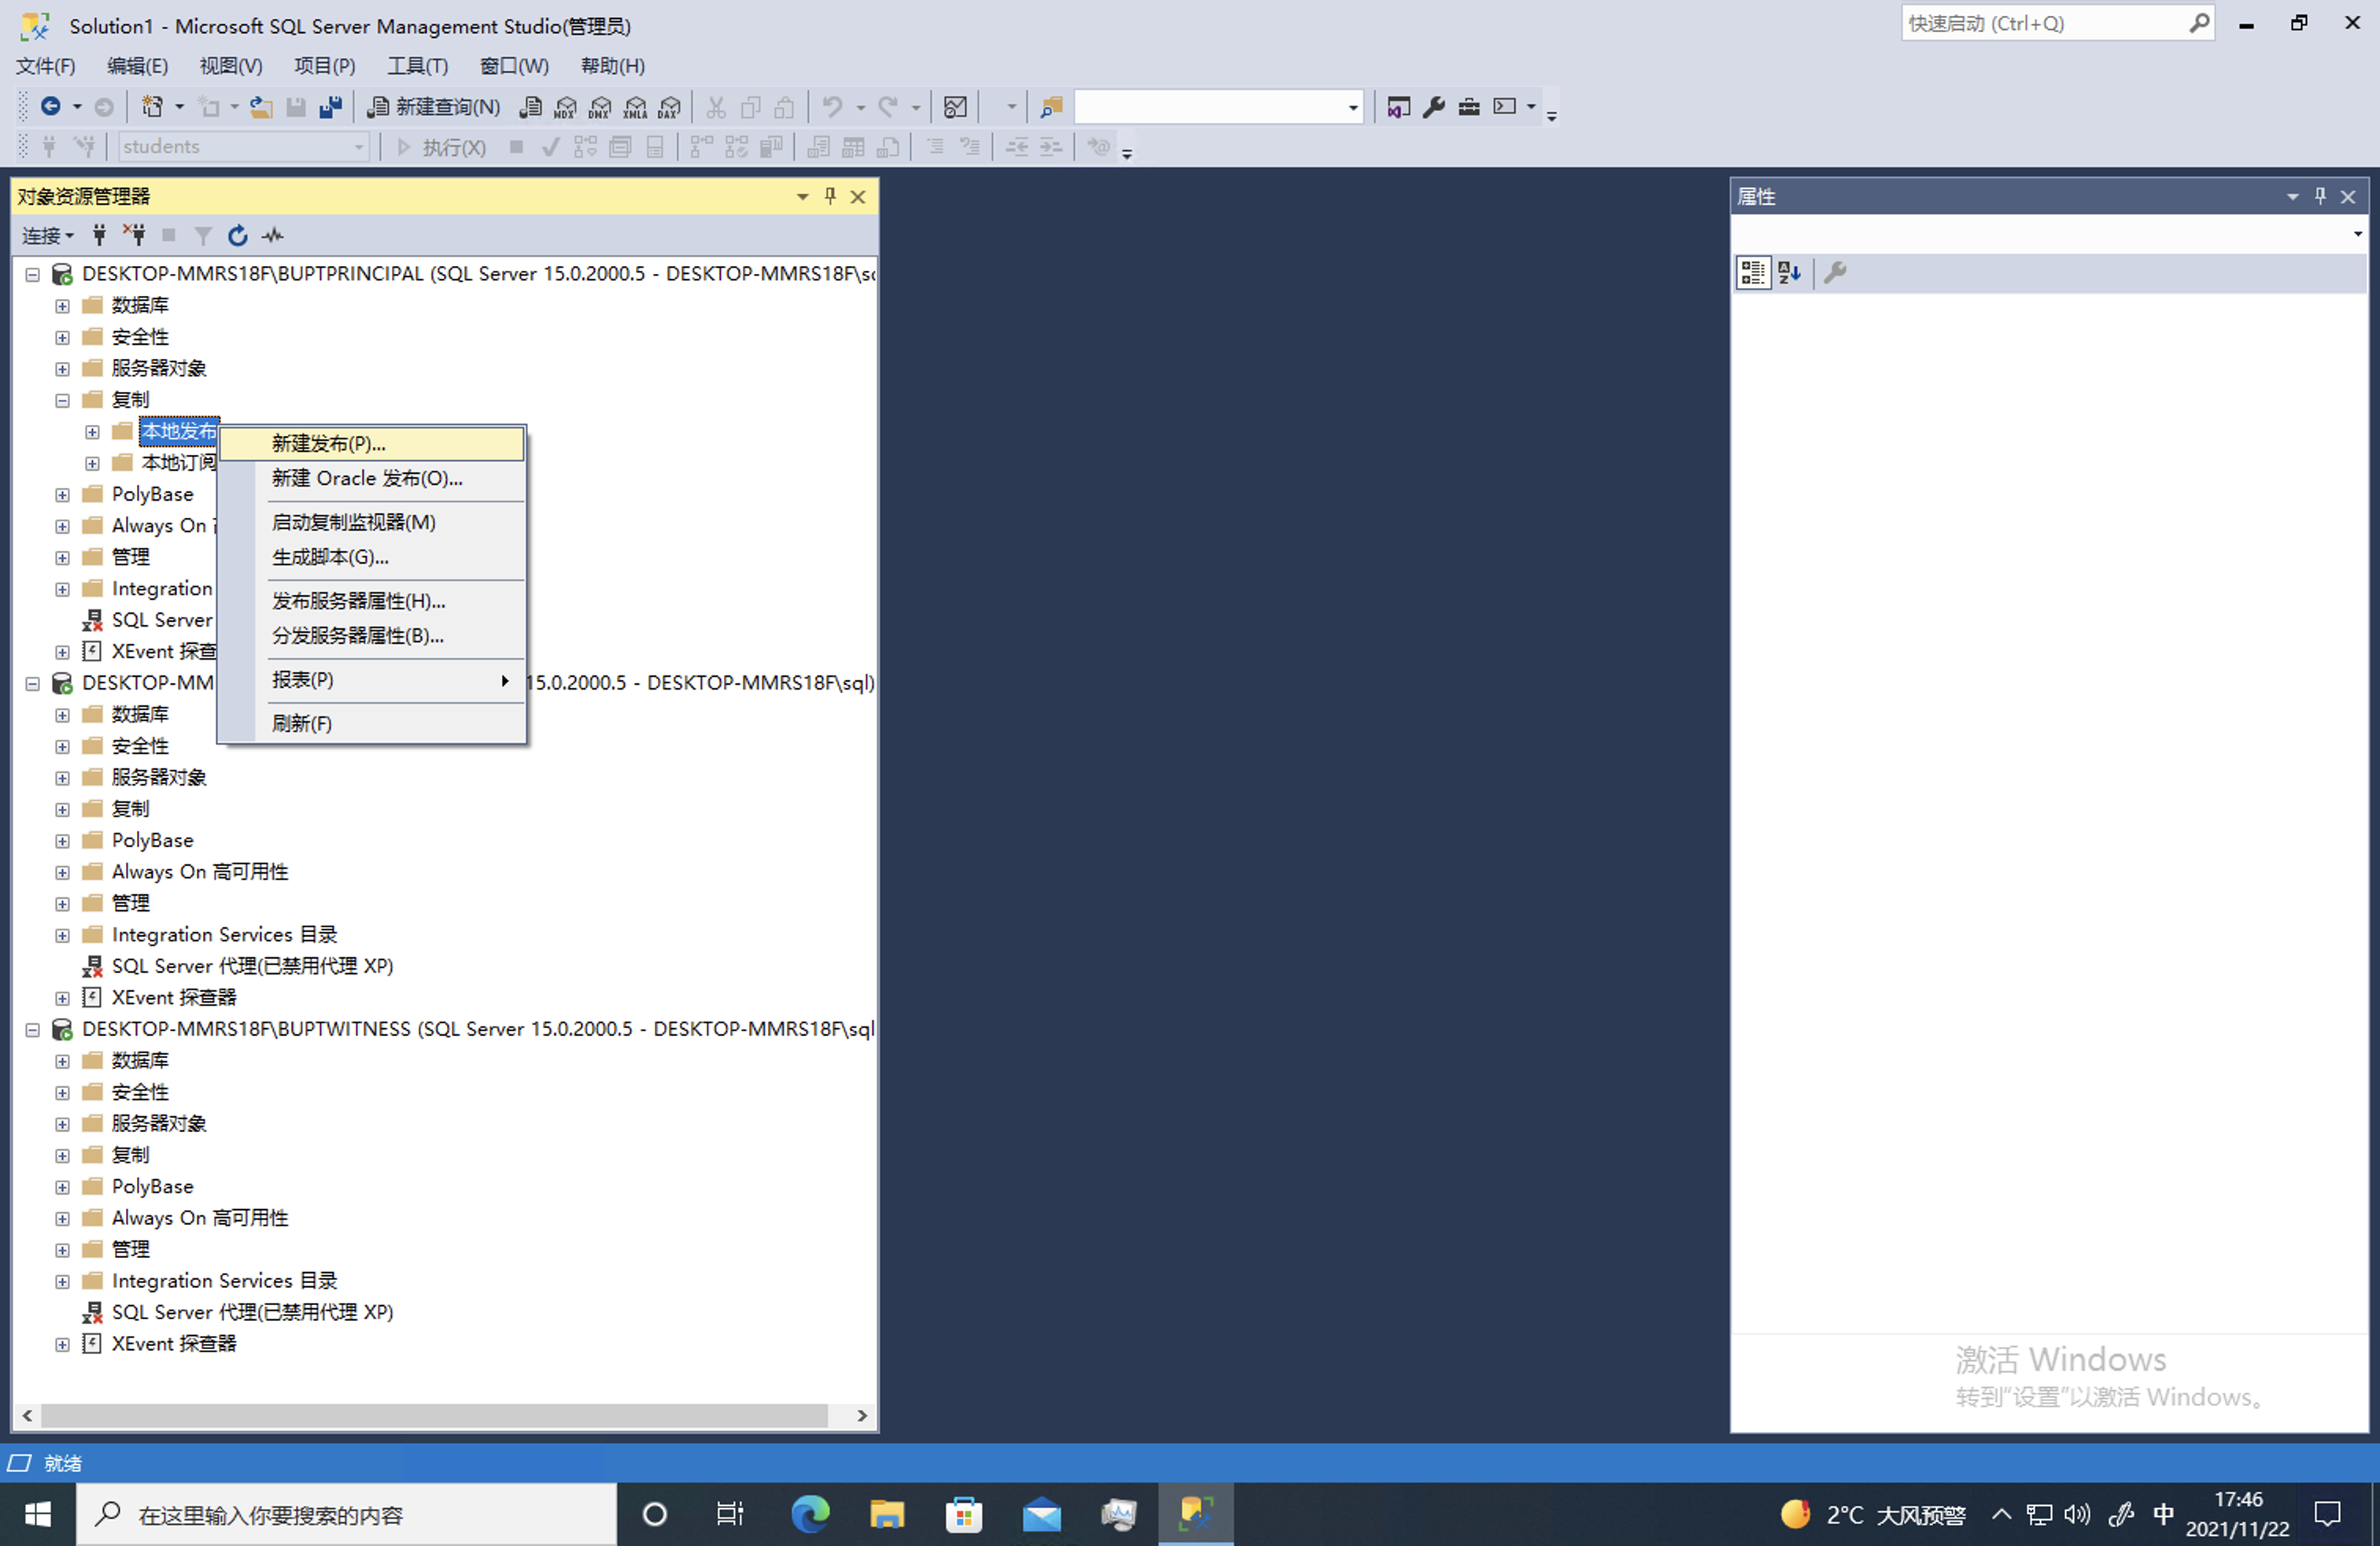
\includegraphics[width=0.70\textwidth]{image/pic18.png}
    \caption{本地发布 -> 新建发布}
    \label{pic18}
  \end{figure}

  \item 快照发布,见Figure \ref{pic19}。

  \begin{figure}[h]
    \centering
    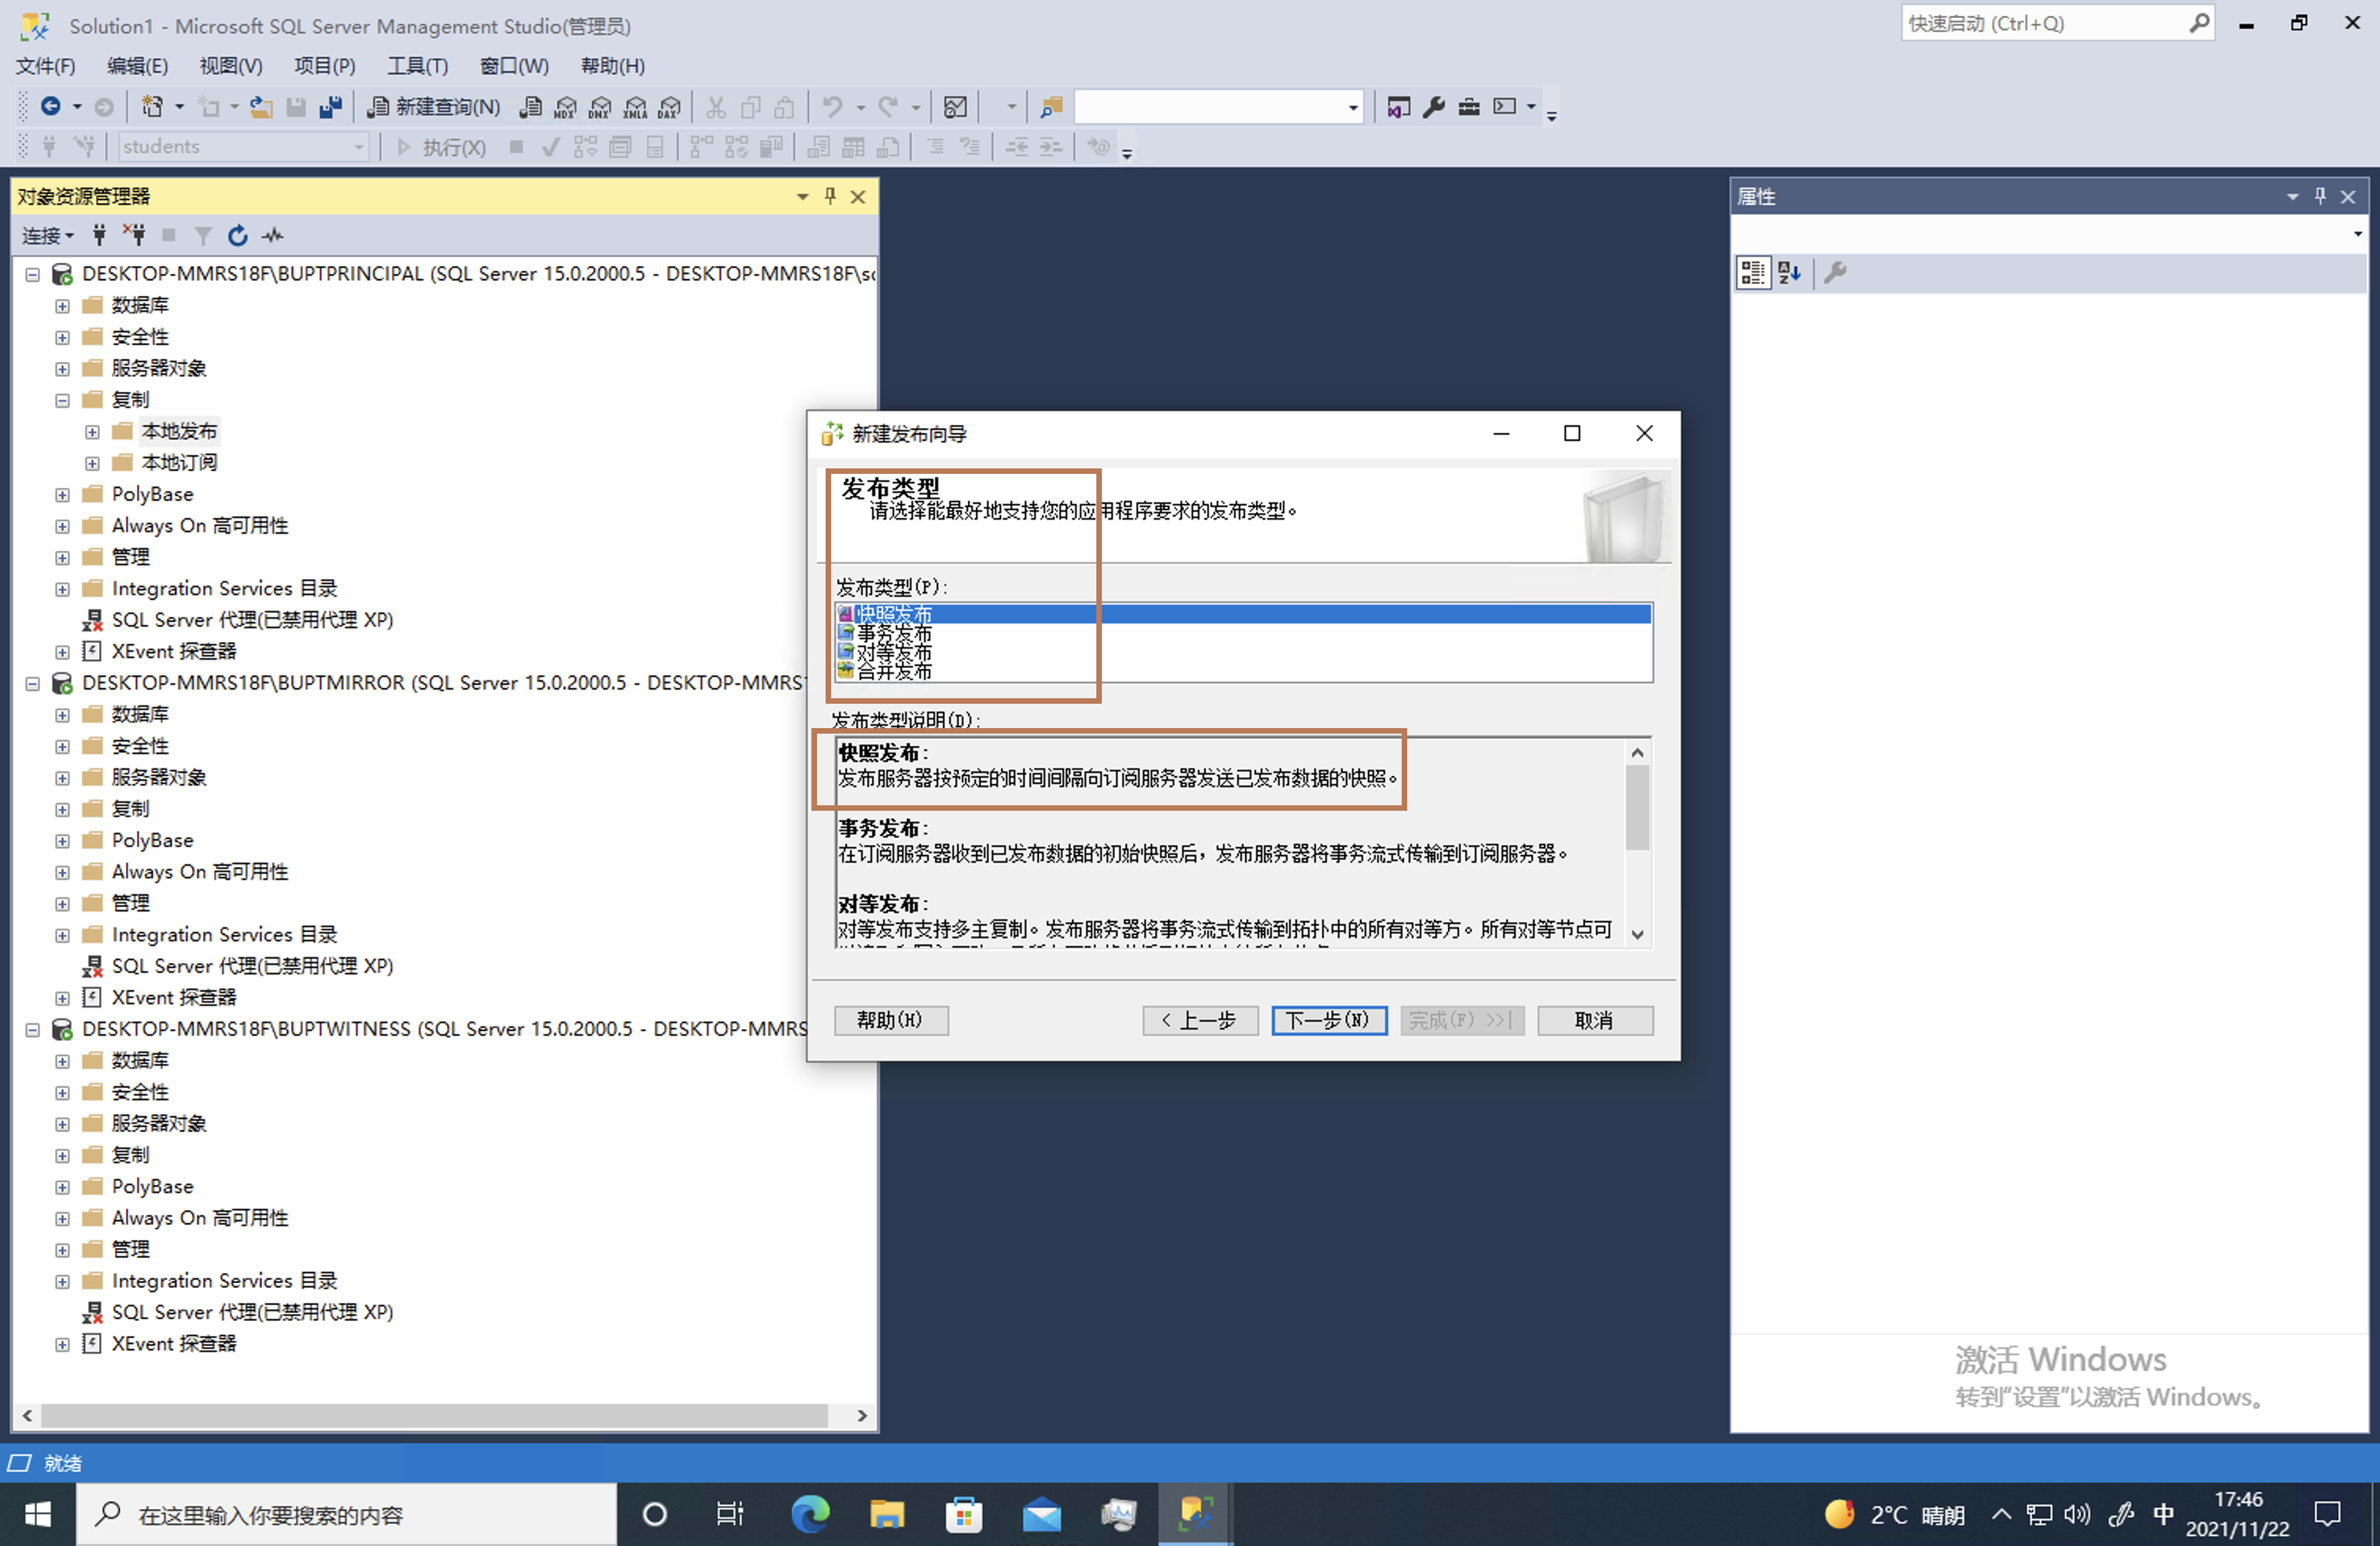
\includegraphics[width=0.70\textwidth]{image/pic19.png}
    \caption{快照发布}
    \label{pic19}
  \end{figure}

  \item 选择快照范围,见Figure \ref{pic20}。
  
  \newpage

  \begin{figure}[h]
    \centering
    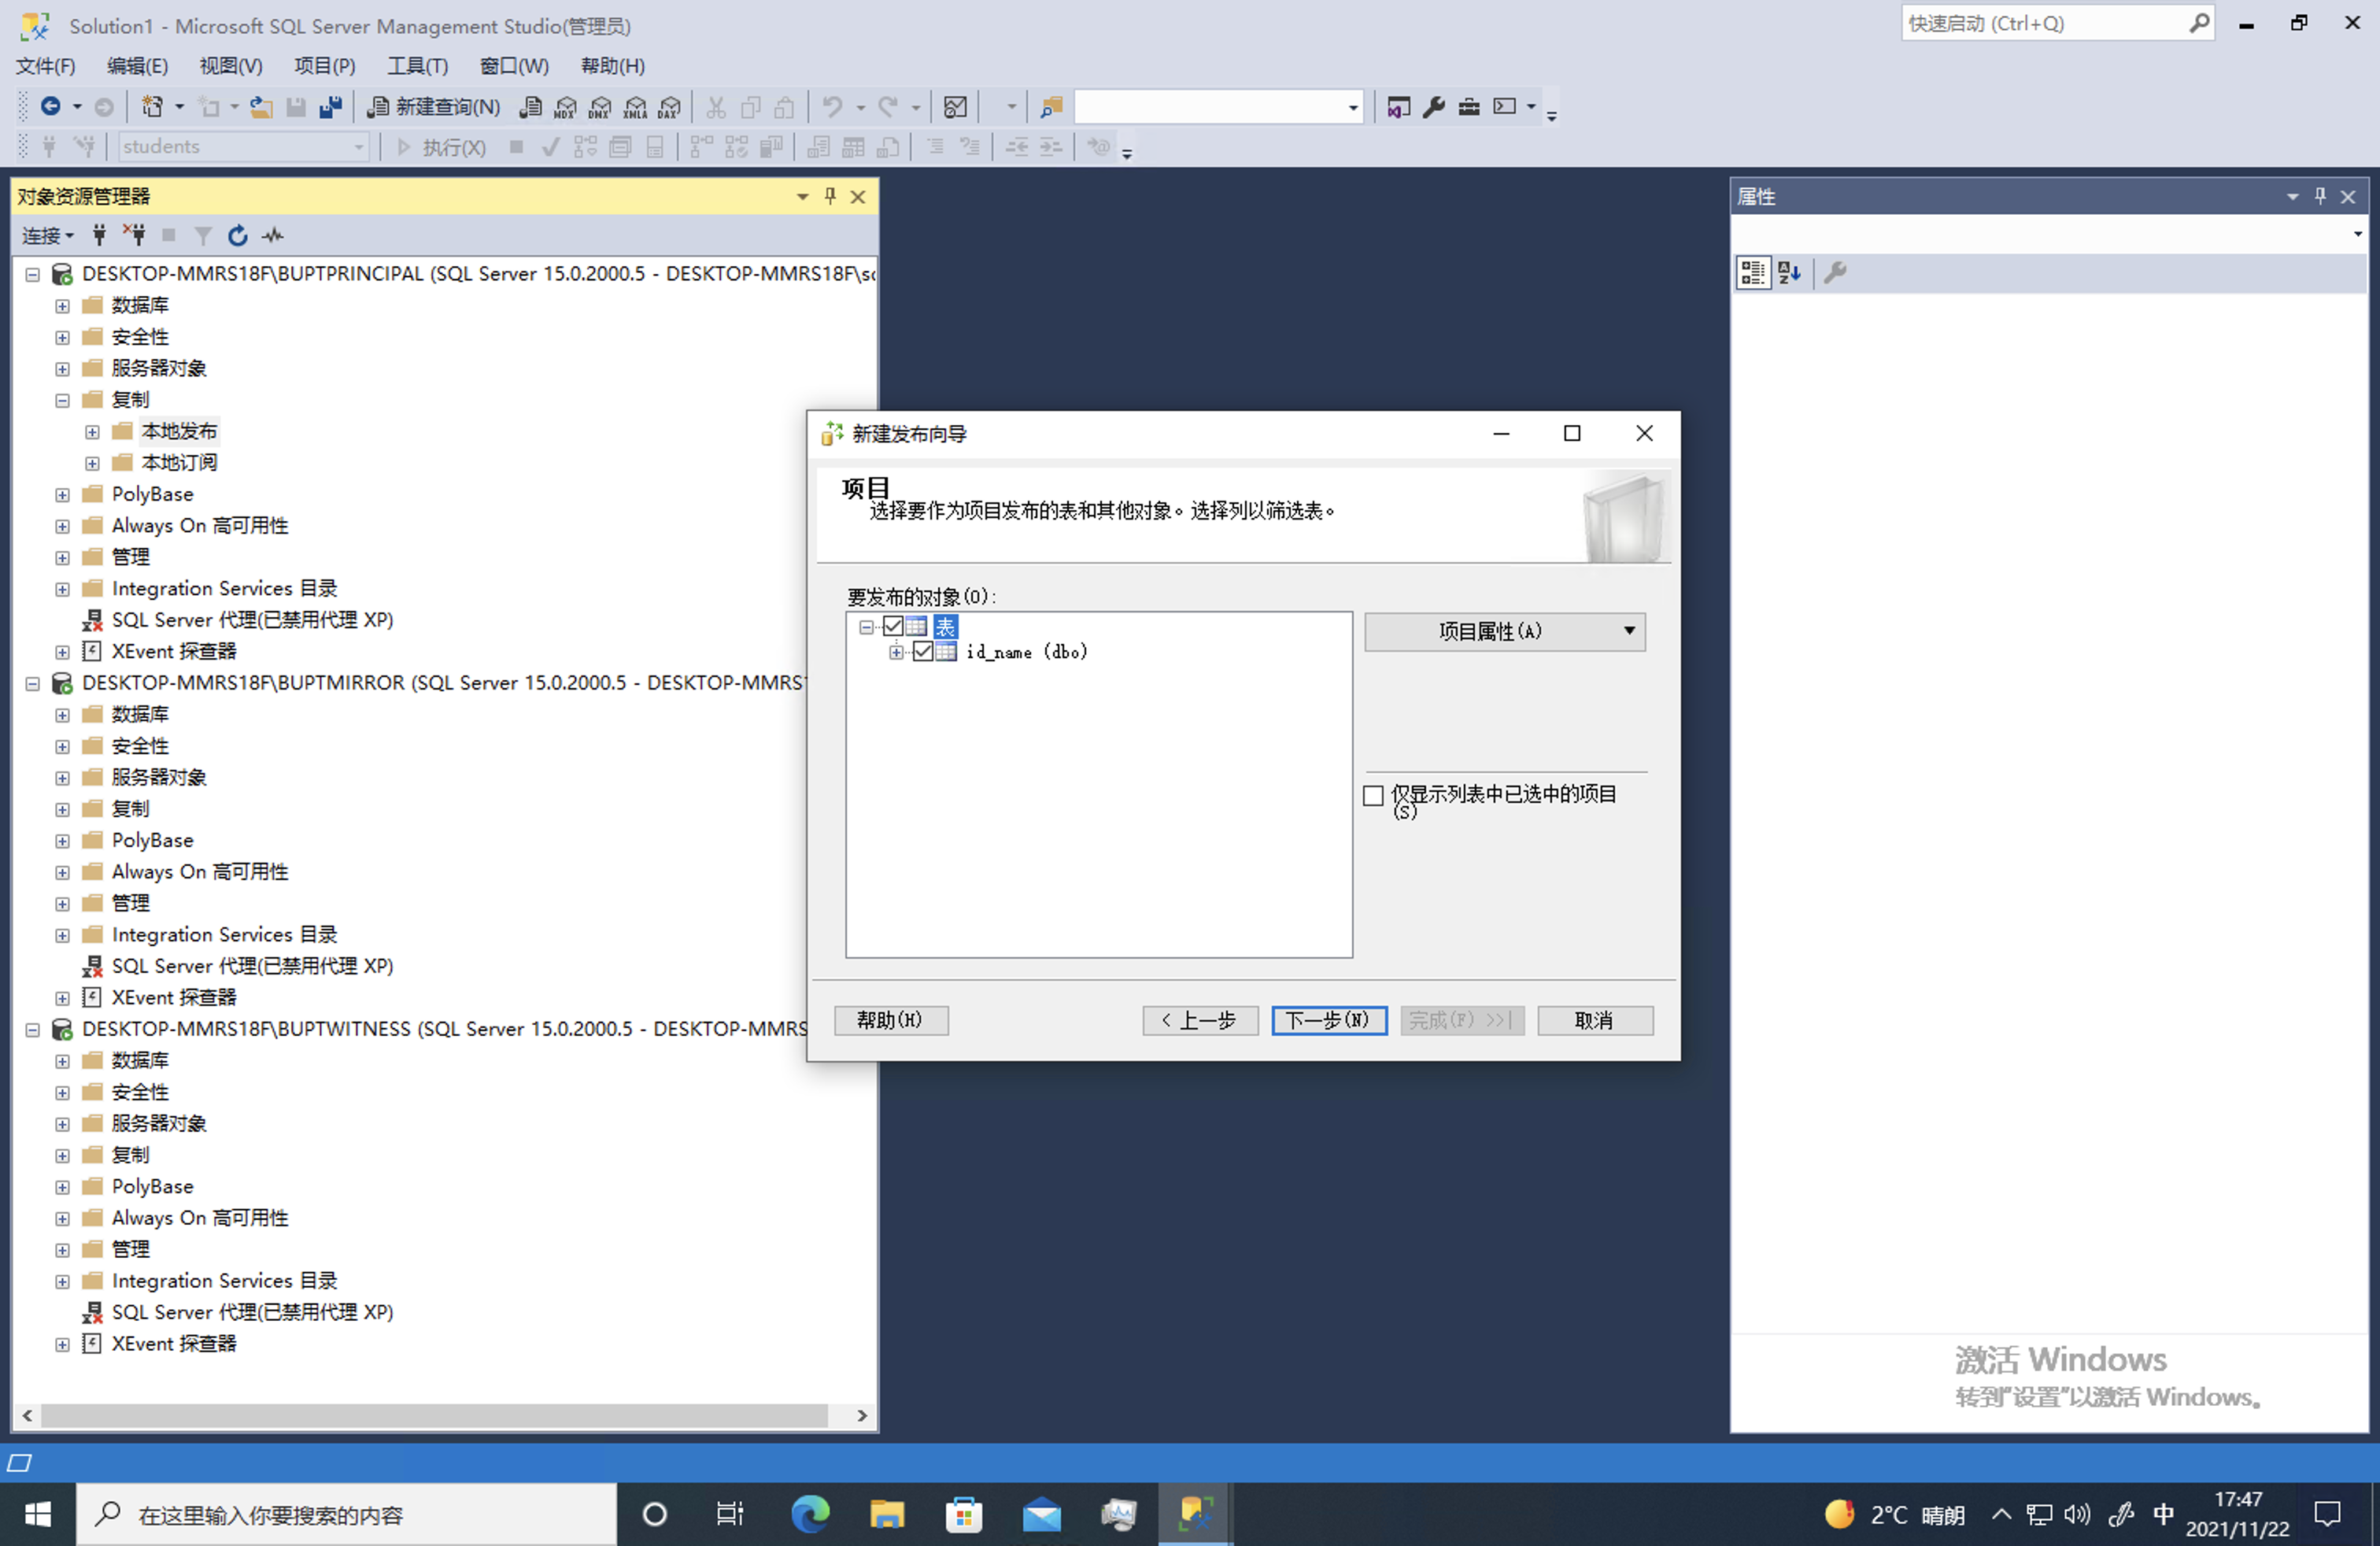
\includegraphics[width=0.70\textwidth]{image/pic20.png}
    \caption{选择快照范围}
    \label{pic20}
  \end{figure}

  \item 设置快照,见Figure \ref{pic21}。

  \begin{figure}[h]
    \centering
    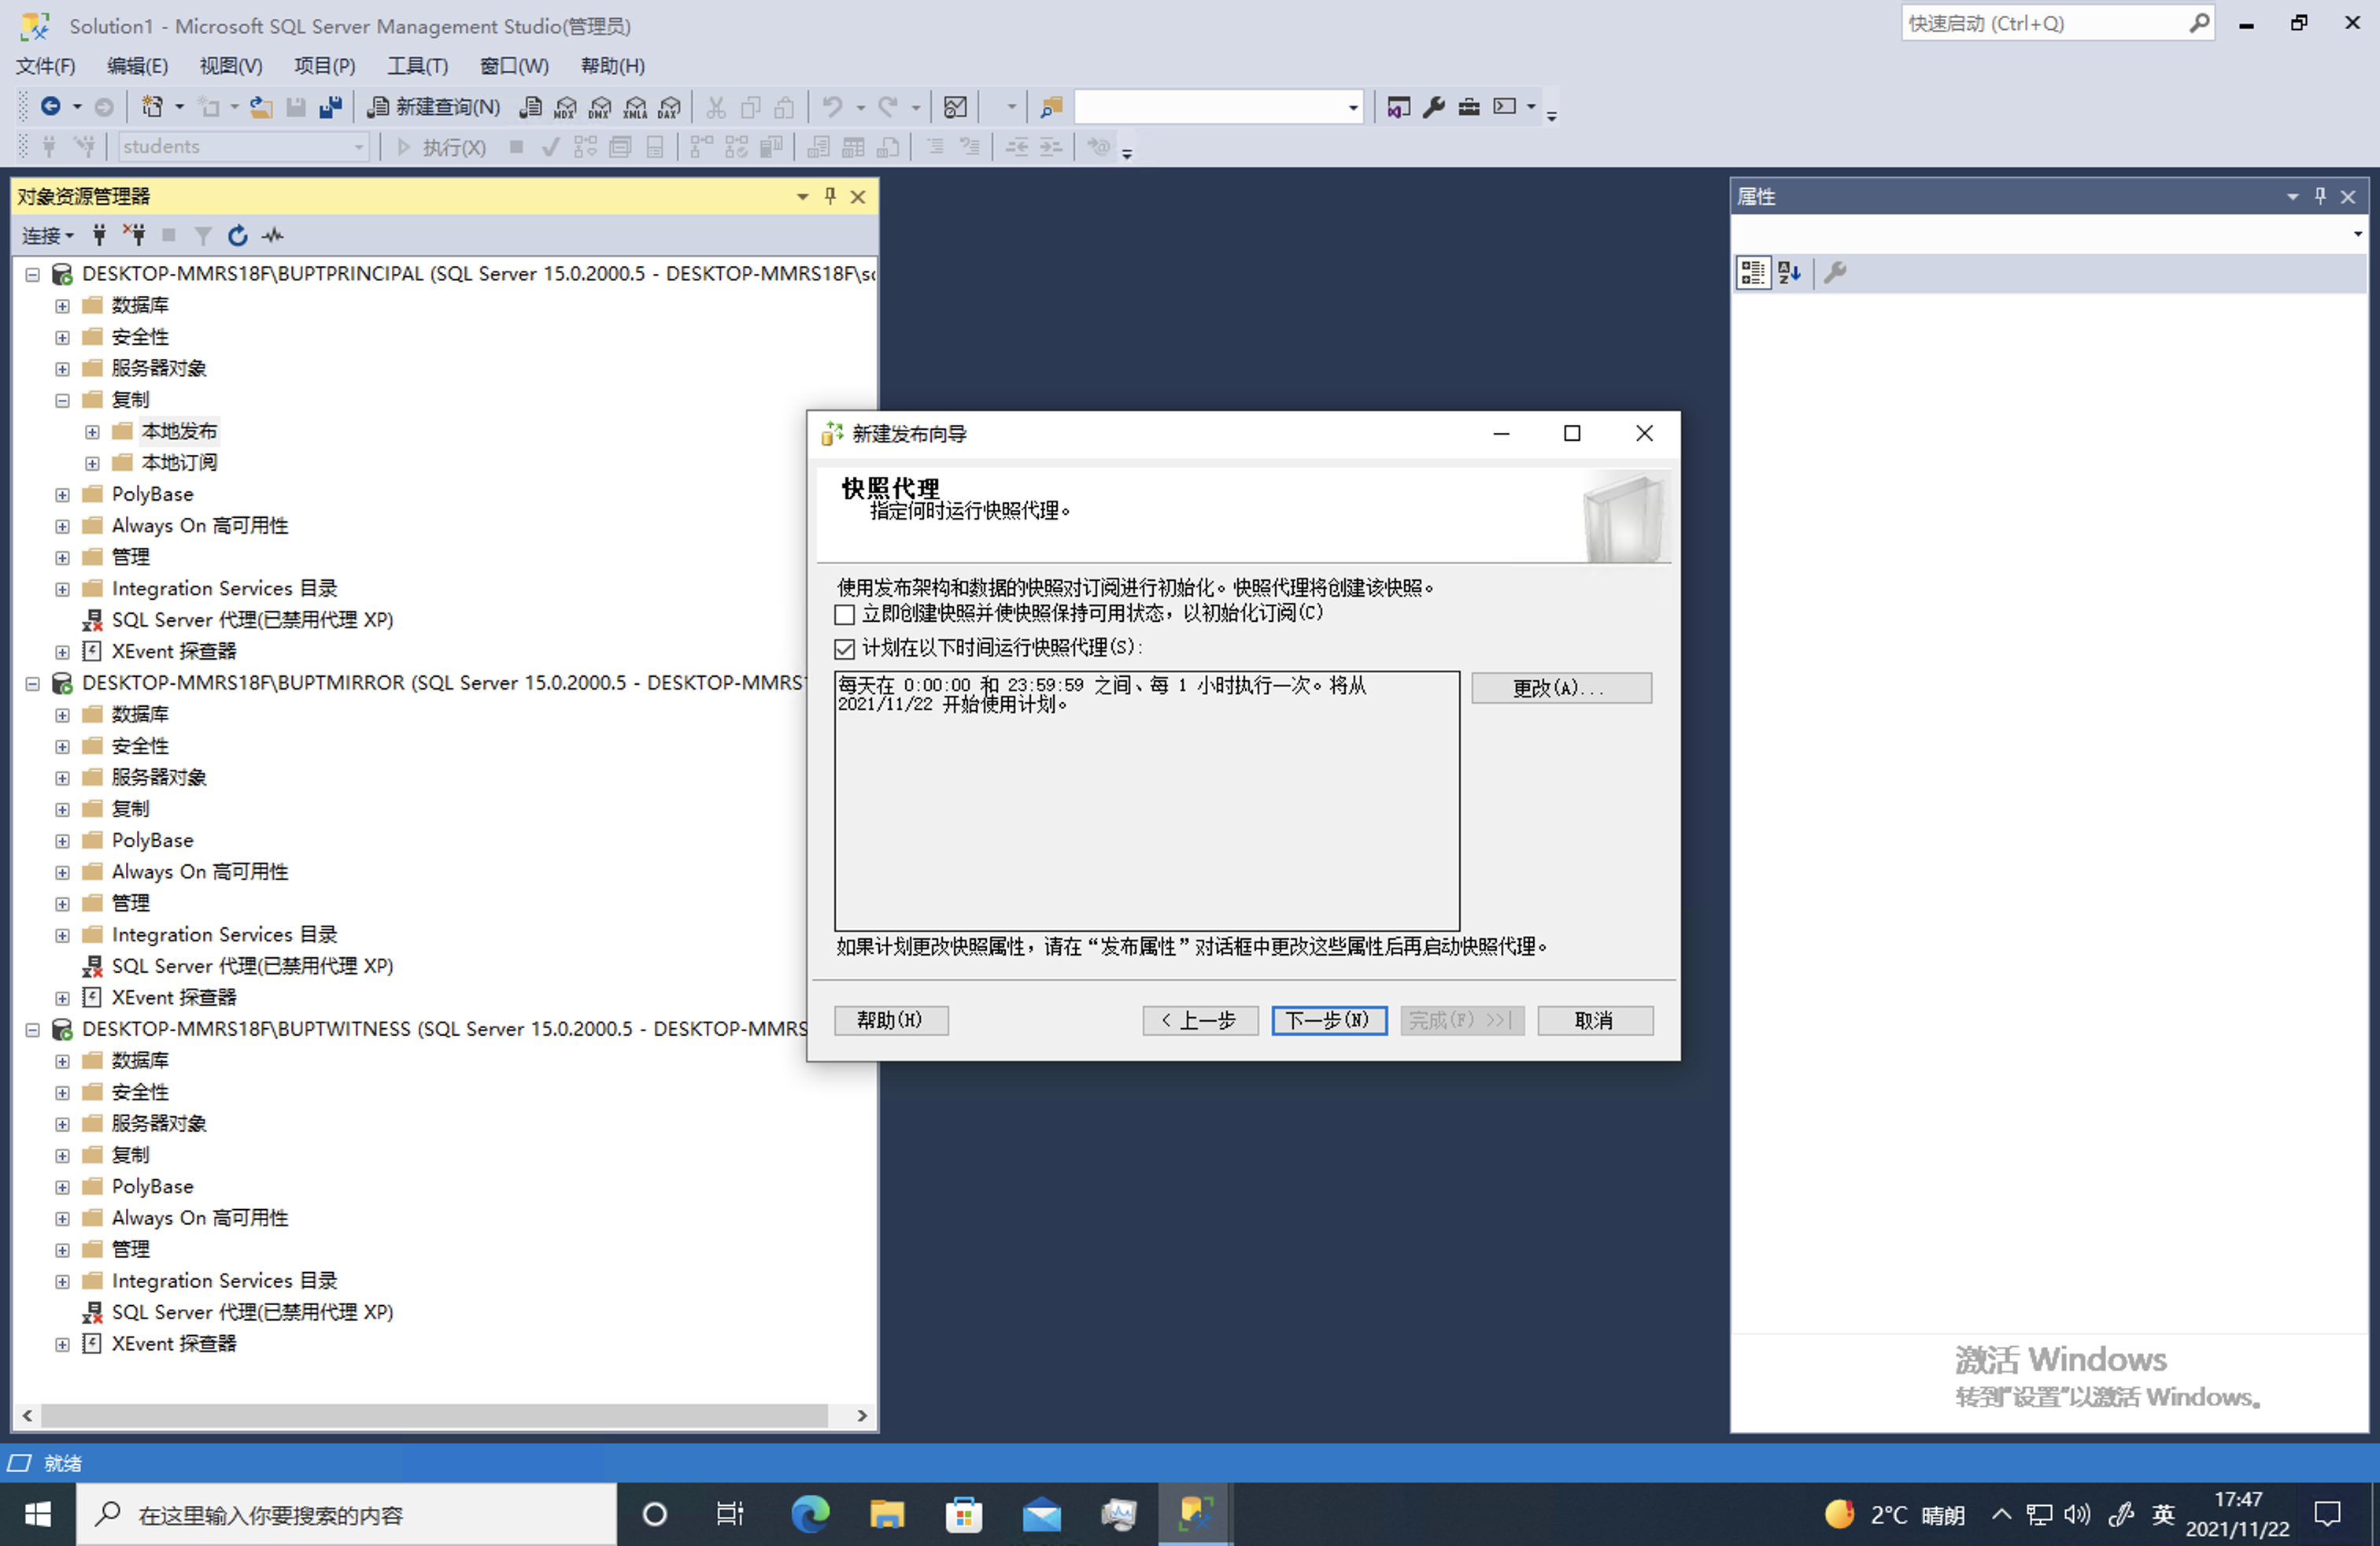
\includegraphics[width=0.70\textwidth]{image/pic21.png}
    \caption{设置快照}
    \label{pic21}
  \end{figure}

  \item 在本地发布找到刚创建的快照,见Figure \ref{pic22}。
  
  \newpage

  \begin{figure}[h]
    \centering
    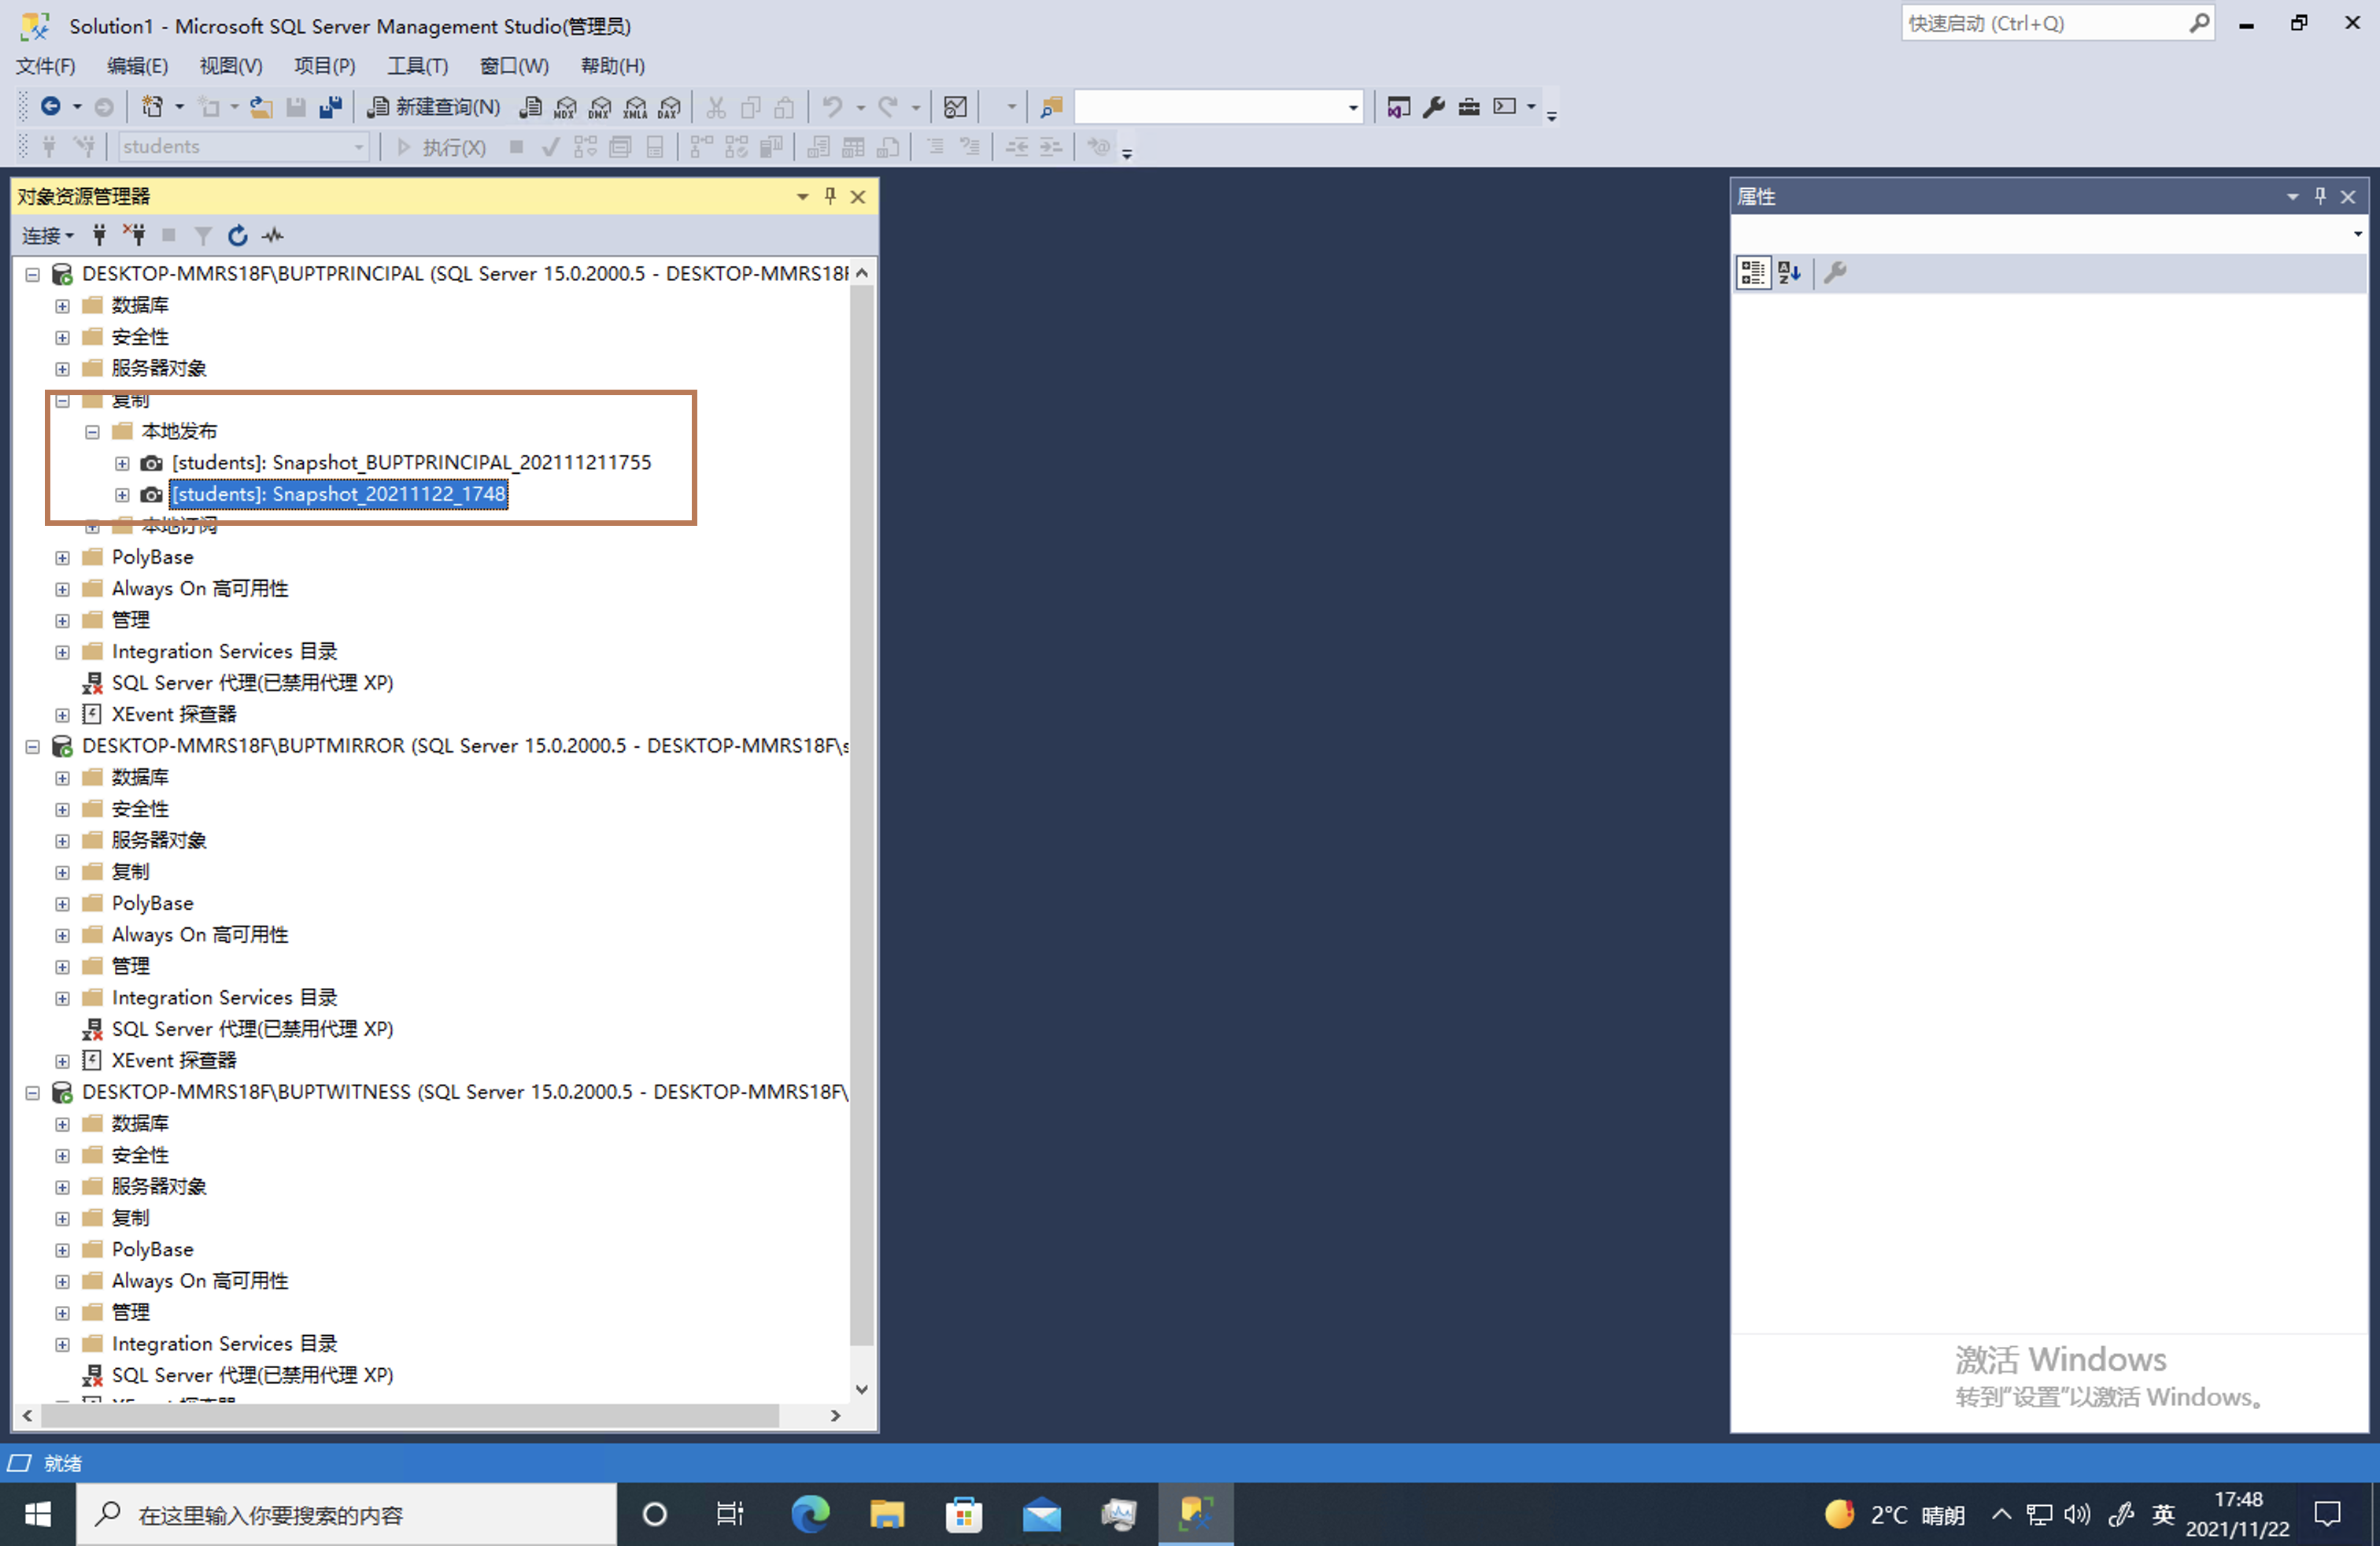
\includegraphics[width=0.70\textwidth]{image/pic22.png}
    \caption{在本地发布找到刚创建的快照}
    \label{pic22}
  \end{figure}

  \end{enumerate}

  \subsection{实验结果测试}

  \begin{enumerate}

    \item 使用另一个SQL Server实例,本地订阅我们主体服务器创建的快照,见Figure \ref{pic23}。
    
    \begin{figure}[h]
      \centering
      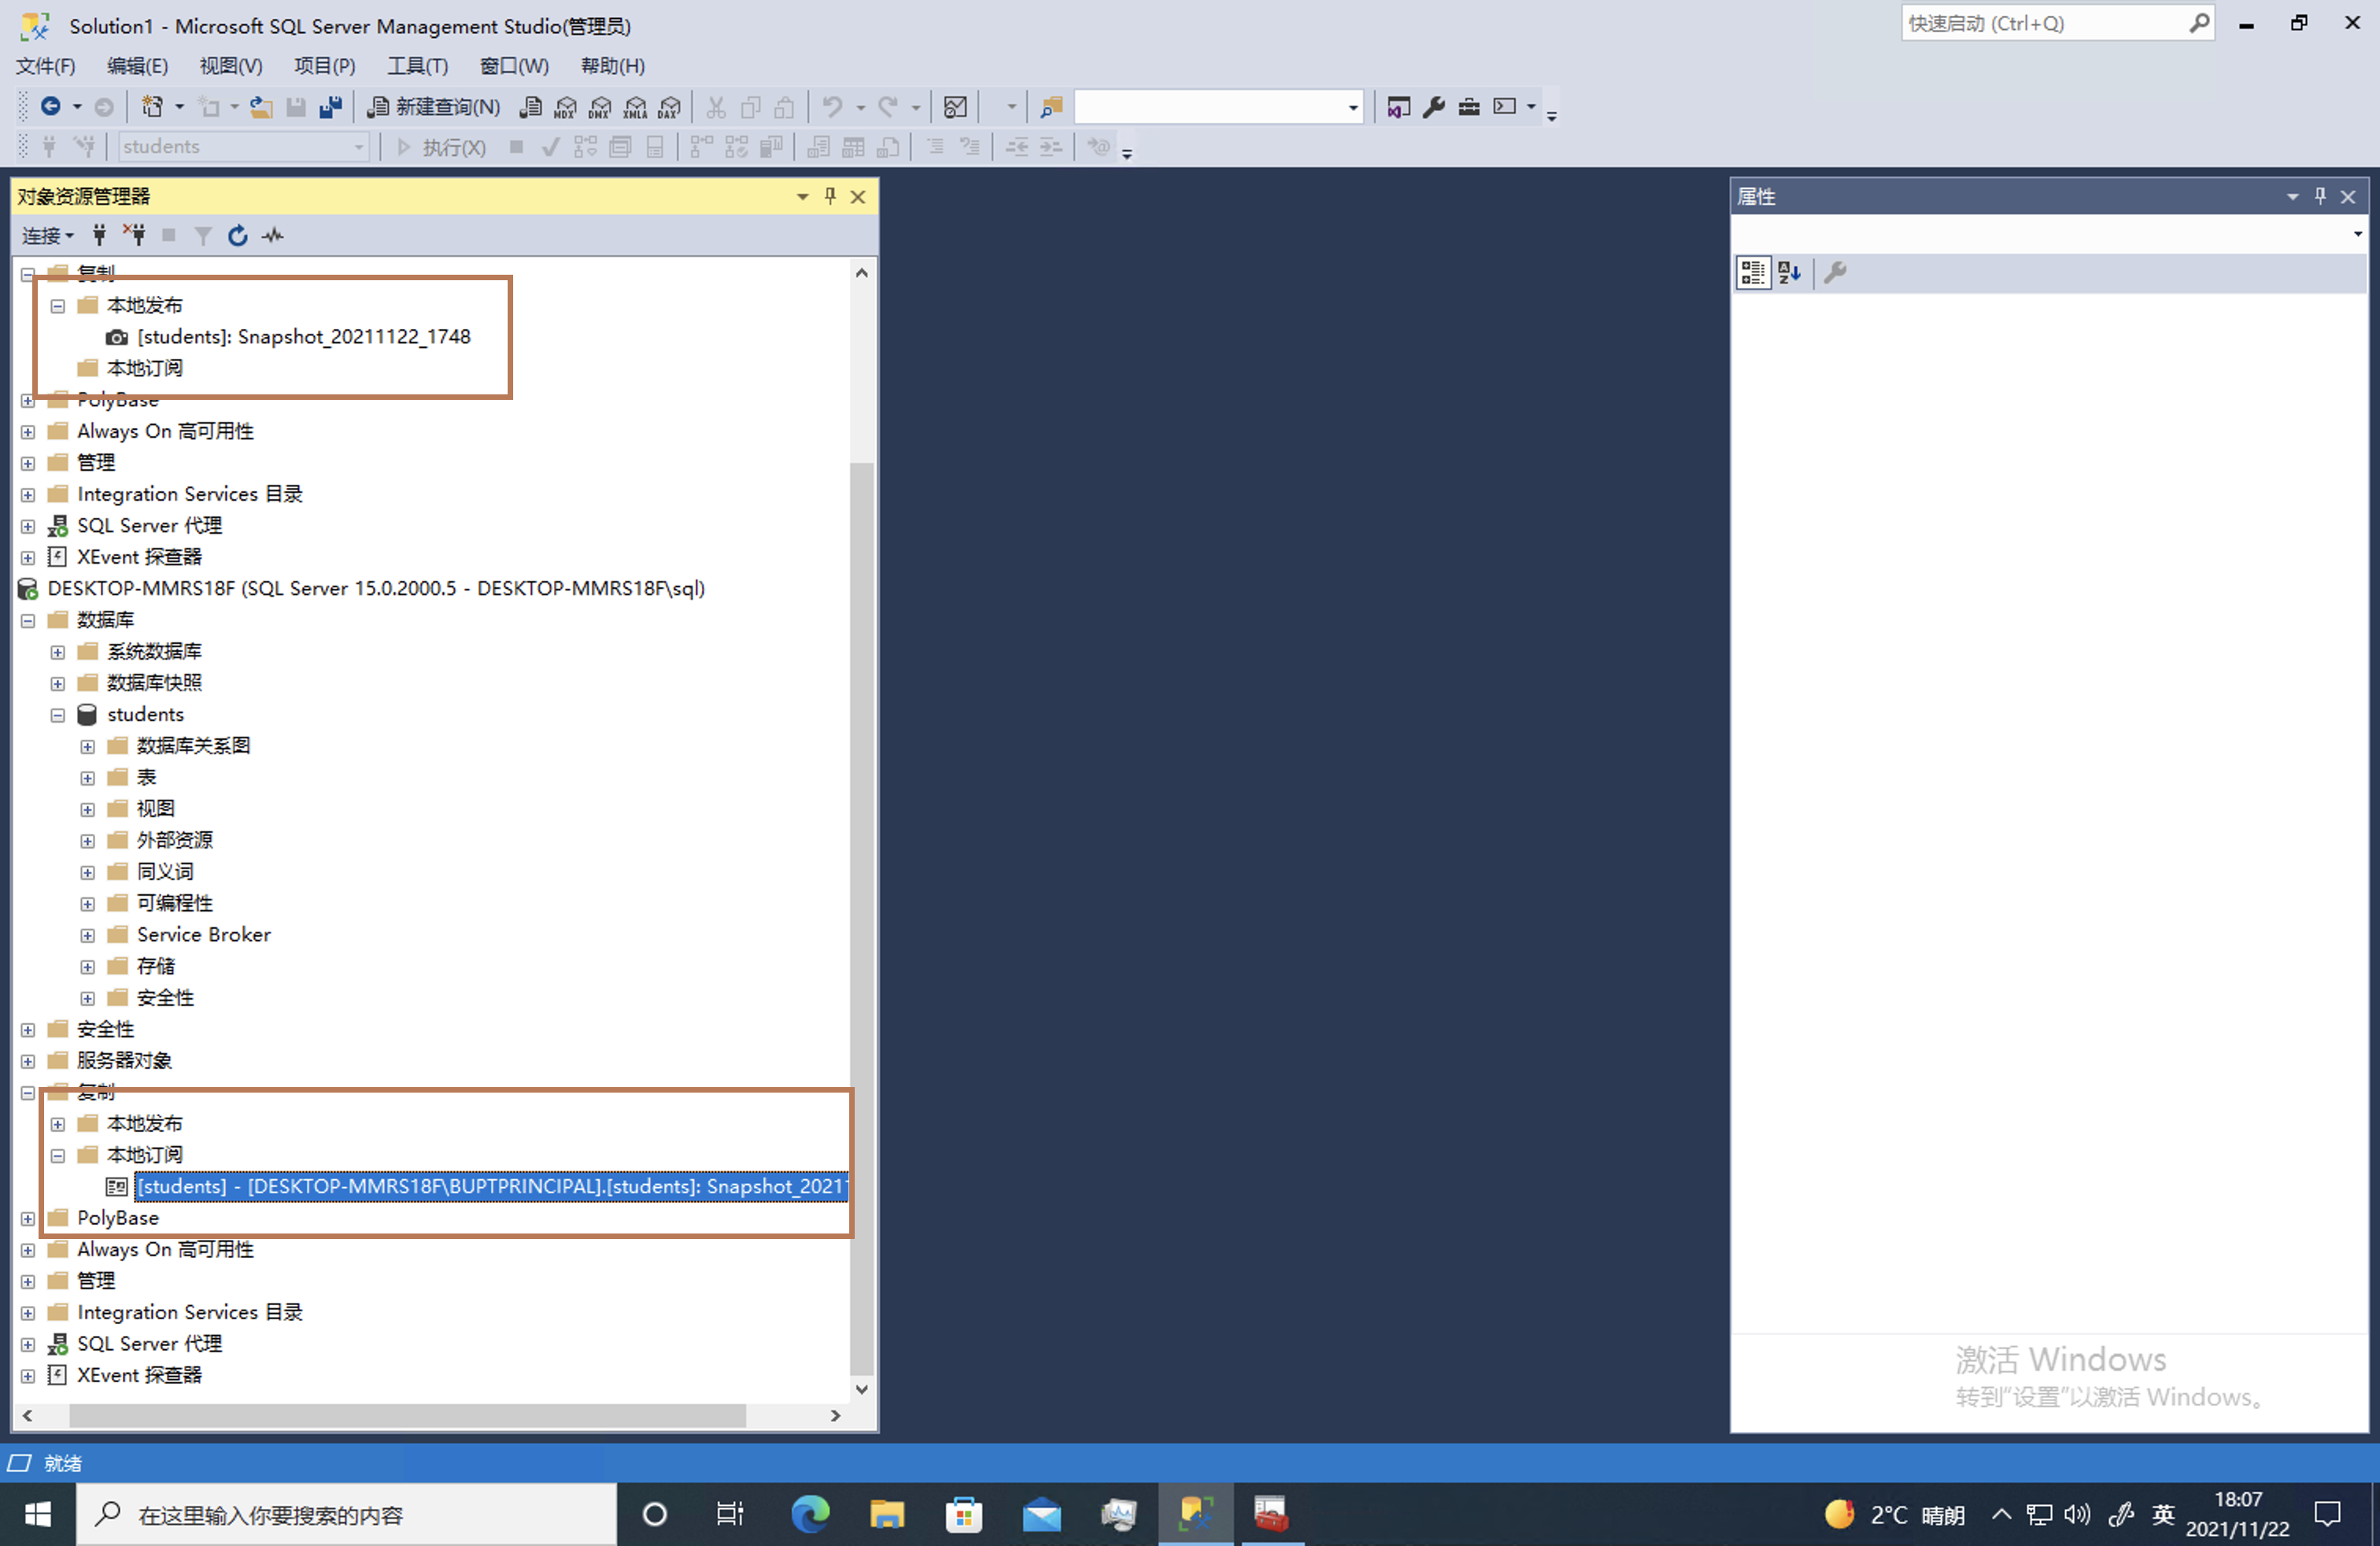
\includegraphics[width=0.70\textwidth]{image/pic23.png}
      \caption{订阅快照}
      \label{pic23}
    \end{figure}

    \item 同步完成,我们可以看到数据和主体数据库的一样,见Figure \ref{pic24}。
    
    \begin{figure}[h]
      \centering
      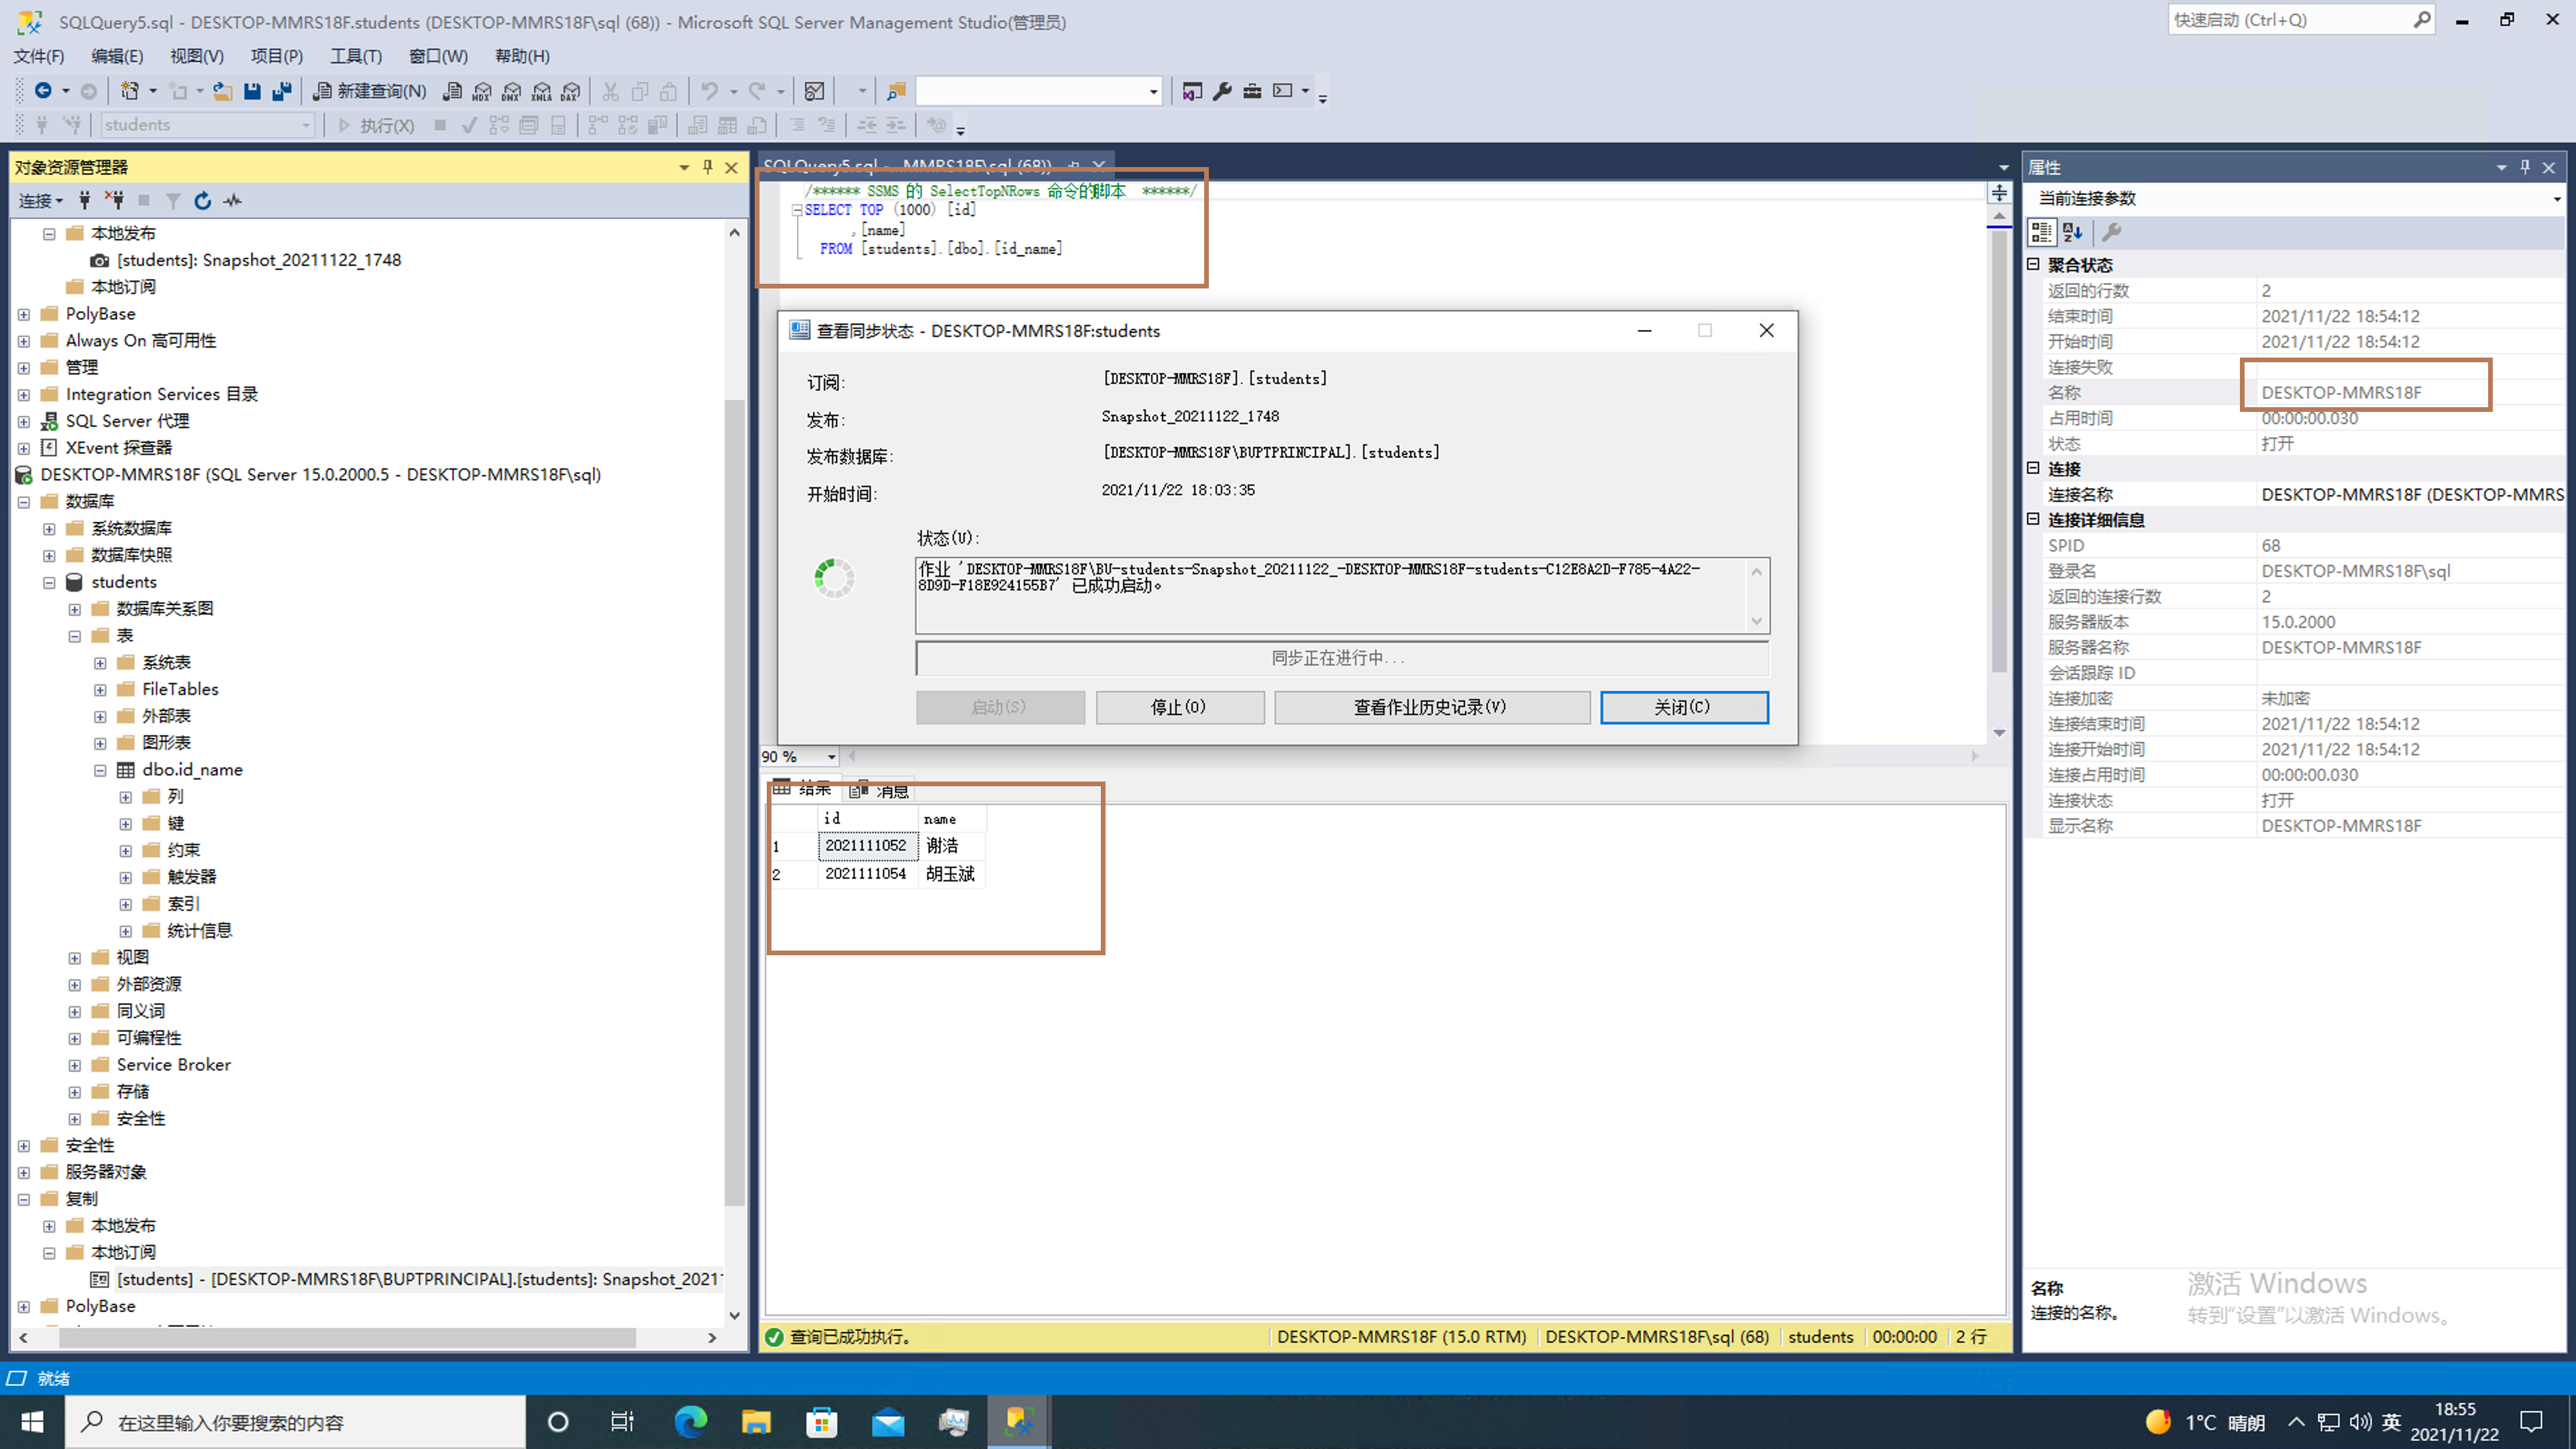
\includegraphics[width=0.70\textwidth]{image/pic24.png}
      \caption{快照后,数据库的数据}
      \label{pic24}
    \end{figure}
    
  \end{enumerate}
  
  \newpage
  \bibliographystyle{ieeetr}
  \bibliography{reference}

\end{document}
